\documentclass[11pt]{article}
\usepackage[T1]{fontenc}
\usepackage{lmodern}
\input{glyphtounicode-cmex}
\pdfgentounicode=1
\pdfinfoomitdate=1
\pdftrailerid{}
\pdfsuppressptexinfo=15
\usepackage[margin=1.08in]{geometry}
\usepackage{amsmath,amssymb,amsthm,mathtools}
\usepackage{microtype}
\usepackage{xcolor}
\usepackage{tikz}
\usetikzlibrary{arrows.meta,positioning,calc}
\PassOptionsToPackage{hyphens}{url}
\hyphenation{Schwarz-schild}
\usepackage[colorlinks=true,linkcolor=blue!45!black,citecolor=blue!45!black,urlcolor=blue!45!black,bookmarksnumbered=true]{hyperref}
\hypersetup{pdftitle={Conformal flow and the Riemannian Penrose inequality with minimizing frontiers},pdfauthor={OpenAI}}
\newtheorem{theorem}{Theorem}[section]
\newtheorem{proposition}[theorem]{Proposition}
\newtheorem{lemma}[theorem]{Lemma}
\newtheorem{corollary}[theorem]{Corollary}
\theoremstyle{definition}
\newtheorem{definition}[theorem]{Definition}
\theoremstyle{remark}
\newtheorem{remark}[theorem]{Remark}
\DeclareMathOperator{\Ric}{Ric}
\DeclareMathOperator{\Hess}{Hess}
\DeclareMathOperator{\tr}{tr}
\DeclareMathOperator{\sym}{sym}
\DeclareMathOperator{\supp}{supp}
\DeclareMathOperator{\divg}{div}
\DeclareMathOperator{\id}{id}
\DeclareMathOperator{\rank}{rank}
\DeclareMathOperator{\Lip}{Lip}
\DeclareMathOperator{\Vol}{Vol}
\DeclareMathOperator{\Area}{Area}
\DeclareMathOperator{\dist}{dist}
\DeclareMathOperator{\sgn}{sgn}
\newcommand{\R}{\mathbb R}
\numberwithin{equation}{section}
\allowdisplaybreaks[1]

\title{Conformal flow and the Riemannian Penrose inequality with minimizing frontiers}
\author{OpenAI}
\date{September 27, 2026}
\begin{document}
\maketitle
\begin{abstract}
We give a detailed conformal-flow proof of the numerical Riemannian
Penrose inequality in every dimension $n\ge3$ for complete
asymptotically flat exteriors with nonnegative scalar curvature and
full compact frontiers that are outer minimizing and locally perimeter
minimizing. The metric extends smoothly through the possibly singular
frontier; neither spin nor frontier connectedness is assumed.
The proof follows the conformal-flow approach of Bray, Bray--Lee,
and Bi--Zhu.
\end{abstract}
\tableofcontents
\section{The inequality and the proof}
\label{sec:rpi:introduction}

The Riemannian Penrose inequality compares the mass of an asymptotically
flat manifold with the total area of its outer minimizing minimal
boundary. Its geometric content is that a large minimal enclosure
requires a correspondingly large mass. Penrose's physical argument
\cite{Penrose1973} related an initial trapped area to the mass remaining
after gravitational collapse: cosmic censorship, area increase, and
settling to a Kerr black hole led to the proposed mass--area bound.
For time-symmetric initial data, the energy condition becomes
nonnegative scalar curvature and the horizon condition becomes
minimality. The resulting Riemannian problem retains the mass--area
comparison without requiring an evolution of the spacetime.

In three dimensions, one route from the horizon to infinity uses the Hawking mass
\cite{Hawking1968}. Geroch's calculation \cite{Geroch1973} showed its
monotonicity along smooth inverse mean curvature flow of two-spheres
in nonnegative scalar curvature. Jang and
Wald \cite[Section~5]{JangWald1977} derived the Penrose bound assuming
a global flow with the required asymptotics. Existence of such a flow
was the central difficulty: mean curvature may vanish and the smooth
evolution can develop singularities. Before the general proofs,
spherical symmetry yielded the inequality \cite{MalecOMurchadha1994},
and spinorial methods gave mass--area estimates involving an additional
normalized Sobolev quantity \cite{Herzlich1997}.

Huisken and Ilmanen's weak inverse mean curvature flow allows jumps
across the regions where smooth flow fails \cite{HuiskenIlmanen2001}.
It proves the sharp mass bound for each connected component of an
outermost minimal boundary in dimension three. Bray's conformal flow
\cite{Bray2001} instead changes the ambient metric while preserving the
total horizon area. Positive mass makes the evolving mass nonincreasing,
and the limiting comparison yields the sharp bound for the full area,
including disconnected boundaries. The harmonic-flat reduction,
area-preserving flow, and mass comparison in the present proof descend
from this construction.

Bray and Lee extended the conformal method to dimensions below eight
\cite{BrayLee2009}. The dimension restriction reflects the use of smooth
minimizing hypersurfaces. In
dimensions at least eight, a minimizing frontier may be singular, and
its singular points affect the flow construction, separation of slices,
and the geometric comparison used to decrease mass.

Restricted all-dimensional results were obtained earlier under
graphical hypotheses. Lam \cite[Corollary~7]{Lam2010Graphs} proved the
inequality for asymptotically flat Euclidean graphs with nonnegative
scalar curvature and convex horizon components. De Lima and Gir\~ao
\cite[Theorem~1.8]{deLimaGirao2015} treated two-sided asymptotically flat
quasi-graphs in Euclidean space, with nonnegative scalar curvature and
convex horizons in a horizontal hyperplane met orthogonally. These
results use additional graphical control of the geometry.

Bi and Zhu \cite[Theorem~1.2]{BiZhu2026v2} prove the all-dimensional
inequality together with Schwarzschild rigidity for almost-minimizing
Caccioppoli (finite-perimeter) boundaries whose regular part is minimal
and which are
their own outermost minimizing enclosures, with a $C^{2,\alpha}$ metric
extension through the boundary. Their version~2 conformal-flow argument
is the immediate framework for this paper. We develop the numerical
proof under stronger local minimization and ambient regularity
hypotheses: the frontier is locally perimeter minimizing on both sides,
the ambient metric is smooth through it, and the scalar curvature has
the pointwise decay stated below. Our initially outer minimizing
frontier is replaced by its outermost hull without changing its area.
The present contribution is a detailed numerical reconstruction
for this minimizing-frontier class.

The reconstruction makes explicit the preservation of area before
limiting nesting, uniform estimates near regular patches of tangent
cones, and complete smooth comparison metrics with positive conformal
factors. It uses only the largest limiting frontier radius to reach
the numerical conclusion. These reductions explain which geometric
and positive-mass inputs suffice without requiring convergence of every
frontier component or classification of equality.

\subsection{Manifolds, frontiers, and mass}

Write $n\ge3$, $k=n-1$, $d=n-2$, and
$\omega=\mathcal H^k_\delta(S^k)$. We use $O_j(r^{-\gamma})$ for a
tensor whose coordinate derivatives of order $\ell\le j$ are
$O(r^{-\gamma-\ell})$. On a Euclidean coordinate end the ADM mass is
\[
 m_{\rm ADM}(h)=\frac1{2k\omega}
 \lim_{R\to\infty}\int_{S_R}
 (\partial_jh_{ij}-\partial_ih_{jj})n_\delta^i\,dA_\delta.
\]
The decay and scalar integrability hypotheses below give the usual
well-defined mass in this normalization; see \cite{Bartnik1986}.

A possibly singular exterior is described by its filled side in a
smooth ambient manifold. The exterior contains the coordinate end; its
compact frontier $\Sigma$ is the support of the perimeter measure of
the filled side. Its area is the full reduced-boundary perimeter,
including every component. The metric extends smoothly through a
neighborhood of $\Sigma$. The exterior includes its closed frontier.
For $p,q\in E$, define the possibly extended length distance
\[
 d_E(p,q)=\inf\{\operatorname{Length}_h(\gamma):
       \gamma\subset E\text{ is a rectifiable path joining }p\text{ to }q\},
 \qquad \inf\varnothing=+\infty.
\]
Completeness means that each finite-distance equivalence class
$\{q\in E:d_E(p,q)<\infty\}$ is complete for the restricted metric.
This does not identify $E$ with the length completion of its open
exterior or assert finite-length access to every singular frontier
point. Every point and component of the full frontier remains included
in $E$, with its full perimeter counted.

The frontier is \emph{outer minimizing} if every finite-perimeter
enclosure of its filled side with compact additional support has at
least its perimeter. It is \emph{locally perimeter minimizing} if
compactly supported changes in sufficiently small neighborhoods,
including changes on either side, cannot reduce perimeter. The latter
condition is stronger than weak stationarity. It is the local
comparison needed in the flow construction. At free regular points
it gives the minimal-hypersurface equation.

\begin{theorem}[Riemannian Penrose inequality with minimizing frontiers]
\label{thm:rpi}
Let $(E,h)$ be a connected complete $n$-dimensional exterior, including
its compact frontier $\Sigma$ in the enclosing-set sense above. Suppose
that $h$ is smooth on $E$ and through $\Sigma$, and that
\begin{enumerate}
\item $R_h\ge0$, $R_h\in L^1(E,dV_h)$, and
      $R_h=O(r^{-n-\beta})$ for some $\beta>0$ on the end;
\item outside a compact set there is exactly one Euclidean coordinate
      end with $h-\delta=O_2(r^{-\tau})$, where $\tau>d/2$;
\item the full frontier is outer minimizing and locally perimeter
      minimizing as the boundary of the filled side. Its regular part
      is a smooth embedded minimal hypersurface, and its singular set
      has Hausdorff dimension at most $n-8$.
\end{enumerate}
Then
\begin{equation}\label{eq:rpi:numerical}
 m_{\rm ADM}(h)\ge\frac12
 \left(\frac{\mathcal H_h^k(\Sigma)}{\omega}\right)^{d/k}.
\end{equation}
\end{theorem}

All boundary components enter the displayed area. Neither spin nor
connectedness of the frontier is assumed. The zero-area case is
included: the density lower bound makes a nonempty locally minimizing
frontier have positive perimeter, so zero area means an empty
frontier and the conclusion is nonnegative mass.

For $3\le n\le7$, the frontier is smooth and the numerical assertion
follows from Bray--Lee's published Theorem~1.4 \cite{BrayLee2009}. Its
numerical part has no spin assumption; spin belongs to the separate equality
assertion there. The scalar decay required in that theorem holds here.
The rest of this paper develops the singular argument for $n\ge8$,
including the reduction from harmonic-flat ends to the stated weaker
asymptotics.

The constant is illustrated by the Schwarzschild--Tangherlini metric
\cite{Tangherlini1963}
\[
 h_m=\left(1+\frac{m}{2r^d}\right)^{4/d}\delta,
 \qquad r\ge(m/2)^{1/d},\quad m>0.
\]
Its inner sphere is minimal, its mass is $m$, and its area is
$\omega(2m)^{k/d}$. Thus it realizes the numerical constant in
Equation~\eqref{eq:rpi:numerical}.

The enclosure lemmas in Section~\ref{sec:g-enclosures} identify full
enclosing area with the area of a minimizing frontier and detach that
frontier from a strict inner barrier. Their geometric conclusions are
used independently in boundary-graph deformations
\cite{CompanionBoundaryGraphs}. Corollary~\ref{cor:g-strict-barrier-penrose}
combines them with Theorem~\ref{thm:rpi} to give a Penrose bound for smooth
strict inner barriers. This passage from enclosing area to a minimizing
frontier also supplies the numerical comparison in
\cite{CompanionSpacetimeNumerical} and the smooth nonnegative-mass
reduction in \cite{CompanionSpacetimeRigidity}.

\subsection{Four quantities that control the proof}

First assume the initial metric $g_0=h$ has a harmonic-flat end,
meaning $g_0=H^{4/d}\delta$ there with $H>0$ Euclidean harmonic and
$H\to1$. Extend $g_0$ smoothly a short distance behind its frontier
and truncate on that buried side at a smooth compact boundary. This
gives an ambient exterior $M$ and an initial filled region $K_0$
containing the buried boundary; the original end exterior is
$M\setminus K_0$. The extension needs no scalar-curvature sign behind
the original frontier.

The flow has metrics $g_t=u_t^{4/d}g_0$ and filled regions $K_t$ with
frontiers $\Sigma_t$ and end exteriors $E_t=M\setminus K_t$.
At infinity $u_t\to e^{-t}$. If $y$ denotes the original end coordinate,
we measure mass in the normalized coordinate $x=e^{-2t/d}y$,
in which the metric tends to $\delta$ at spatial infinity for each
fixed $t$.
Four quantities organize the proof:
\[
 A=P_{g_t}(K_t),\qquad m(t)=m_{\rm ADM}(g_t),\qquad
 \mu(t)=m(t)-c_t,\qquad R_t\quad\text{(outer radius)}.
\]
For the radius, represent the compact core by the ball of radius
$R_0e^{-2t/d}$ when the original chart starts at $|y|=R_0$; $R_t$ is
the maximum radius of the union of that ball and the frontier portion
in the normalized chart. The capacity
$c_t=\mathfrak c(\Sigma_t,g_t)$ in the deficit $\mu(t)$ is the
normalized energy of the harmonic function $w_t$
equal to one at the conductor and zero at infinity:
\[
 \mathfrak c(\Sigma_t,g_t)=\frac1{d\omega}
 \int_{E_t}|dw_t|_{g_t}^2\,dV_{g_t}.
\]
The flow keeps $A$ fixed and satisfies $m'=-2\mu$ almost everywhere.
The mass--capacity comparison gives $\mu\ge0$; a one-sided time estimate
then gives $\mu(t)\to0$. The limiting harmonic potential identifies
the largest limiting frontier radius, and enclosing
spheres give the sharp area inequality.

The constructions establishing these facts have a necessary order.
Section~\ref{sec:g-enclosures} states the independent enclosure results;
their proofs are collected in Section~\ref{sec:g-enclosure-proofs},
where they enter the final approximation argument. In
Sections~\ref{sec:rpi:flow-localization}--\ref{sec:rpi:flow-construction},
the discrete flow supplies uniform density and potential estimates.
We prove preservation of the limiting minimum area before deriving
nesting of the limiting outermost hulls. This follows the order in
Bi--Zhu version~2, Lemmas~2.21 and~2.23 and Corollary~2.22
\cite{BiZhu2026v2}.

For mass--capacity comparison we need a smooth boundary separated from
the singular frontier. Sections~\ref{sec:rpi:regular-patches}--\ref{sec:rpi:median-separation}
use a single median of the distance between frontiers to normalize all
regular patches and prove this separation. The method descends from the
singular maximum principles of Simon and Ilmanen
\cite{Simon1987Maximum,Ilmanen1996Maximum}, as developed in
\cite[Section~4]{Wickramasekera2014Maximum}, and adapts Bi--Zhu's relative
forcing and normalization \cite[Proposition~2.34 and Lemma~2.35]{BiZhu2026v2}.
Section~\ref{sec:rpi:smoothing} then smooths on the exterior side while
retaining the curvature sign, following the distance-offset strategy
of \cite{BiZhuSmoothing2026}.

Before applying positive mass, Sections~\ref{sec:rpi:smooth-repair} and
\ref{sec:rpi:lee-completion} construct complete smooth comparison metrics.
Brendle--Wang's theorem \cite[Corollary~1.6]{BrendleWang2026} requires
strictly positive scalar curvature and an all-order end expansion.
From it we obtain nonnegative mass on harmonic-flat ends and
mass--capacity comparison by doubling and collar repair \cite{Miao2002}.
A one-end reduction then permits the quantitative estimate of Lee
\cite{Lee2007NearEquality}. Appendix~\ref{sec:rpi:weighted-minimizers}
proves a local weighted-minimizer estimate using \cite{NaberValtorta2020}
to substantiate singular-set control in that positive-mass method.
The smooth positive-mass theorem itself remains an independent input.

Finally, Section~\ref{sec:rpi:numerical-limit} identifies the limiting
outer radius and completes the harmonic-flat argument.
Section~\ref{sec:rpi:density-repair} first creates a strict smooth inner
barrier and then approximates the general end, controlling both mass
and every enclosing area. Thus the approximation does not require a
theorem preserving a singular minimal frontier.

\paragraph{Mean-curvature convention.}
At an inner frontier, $\nu$ points toward the asymptotic end and
$H_\nu=\operatorname{div}_\Sigma\nu$. The outward normal of the exterior
region is $-\nu$. Mean-curvature signs below are always stated using
one of these explicit normals.

\section{Full enclosures and smooth obstacles}
\label{sec:g-enclosures}

A smooth inner boundary need not minimize the area of its enclosures.
The three lemmas in this section replace it by a full minimizing
frontier, retaining every component and every portion of contact with
the original boundary. A strictly negative inner mean curvature then
makes the minimizing frontier detach from that boundary. These are
geometric results for a fixed smooth metric; they require neither
nonnegative scalar curvature nor a mass hypothesis.

We state the results here for later reference.
Their proofs are given together in Section~\ref{sec:g-enclosure-proofs},
immediately before their use in the passage from harmonic-flat to
general asymptotically flat ends. The local obstacle regularity is the
same input that underlies minimizing hulls in Huisken--Ilmanen's
inverse mean curvature flow \cite{HuiskenIlmanen2001}.

\subsection{The full area and its minimizing enclosure}

Let $(X,g)$ be a smooth connected Riemannian manifold of
dimension $n\ge3$, complete with its nonempty compact smooth boundary
$B$ included.  Assume that $X$ has one coordinate end with compact
complement and that, in its coordinates,
\begin{equation}
 g_{ij}-\delta_{ij}=O_2(r^{-q})\qquad\text{for some }q>0.
 \label{eq:g-end}
\end{equation}
Only the eventual strict mean convexity of its coordinate spheres is
needed for the three enclosure lemmas below. In particular, scalar
curvature and ADM mass play no role in those lemmas.

A \emph{full smooth enclosing cut} is the entire intrinsic manifold
boundary $\partial_{\mathrm{man}}D$ of a connected smooth domain
$D\subset X$ that is closed in $X$, contains the distant coordinate
end, and has compact boundary.  Its intrinsic interior must lie in
$\operatorname{int}X$.  All boundary components and every portion
coincident with $B$ are counted.  Thus $D=X$ is admissible and its cut
is $B$.  Define
\begin{equation}
 a_g(B)=\inf_D\operatorname{Area}_g(\partial_{\mathrm{man}}D).
 \label{eq:g-full-cut-area}
\end{equation}

Attach a compact smooth filling $O$ behind $B$ and extend $g$ smoothly
across $B$, obtaining a connected boundaryless manifold $M$ with
$M\setminus O=\operatorname{int}X$.  Such a filling exists: take a
second copy of a compact truncation of $X$, reverse the collar
direction along $B$, and cap its spherical end boundary with a ball.
This construction does not require an orientation.  The extension
is auxiliary; it will not change any area in
\eqref{eq:g-full-cut-area}.  Since the attached part is compact, the
extended metric can and will be chosen complete.

Let $\mathcal A$ be the bounded finite-perimeter subsets $E$ of $M$
that contain $O$ up to a volume-null set.  Sets agreeing almost
everywhere are identified.  If $\partial^*E$ denotes the reduced
boundary and $\nu_E$ its measure-theoretic outward unit normal, set
\begin{equation}
 P_g(E)=|D\mathbf1_E|_g(M)
       =\mathcal H^{n-1}_g(\partial^*E).
 \label{eq:g-full-perimeter}
\end{equation}
This is perimeter in the extended manifold.  In particular
$P_g(O)=\operatorname{Area}_g(B)$.  Relative perimeter in
$\operatorname{int}X$ would instead assign zero to $O$ and would lose
all contact area.  We use the standard compactness, approximation,
trace, and Gauss--Green results for finite-perimeter sets
\cite{AmbrosioFuscoPallara2000,Maggi2012}.

\begin{lemma}[The full enclosure minimum]
\label{lem:g-enclosure}
Under the preceding hypotheses,
\begin{equation}
 0<a_g(B)=\min_{E\in\mathcal A}P_g(E)
         \le\operatorname{Area}_g(B).
 \label{eq:g-minimum}
\end{equation}
All minimizers are supported in one compact subset of $M$.  The family
of minimizers is compact for $L^1(M)$ convergence, and that convergence
also entails convergence of their full perimeters.

Each minimizer has a closed representative $E$ whose frontier is
$T=\operatorname{supp}|D\mathbf1_E|_g$.  Its exterior $M\setminus E$
is connected and contains the distant end.  There are full smooth
enclosing cuts in $\operatorname{int}X$ with areas tending to $P_g(E)$.
When $3\le n\le7$, these cuts can be chosen to converge to $T$ in
$C^1$.  Every minimizer is outer minimizing: if $F\supset E$ is
bounded and has finite perimeter, then $P_g(F)\ge P_g(E)$.
\end{lemma}

The proof in Section~\ref{subsec:g-proof-enclosure} identifies the
perimeter minimum with the infimum over full smooth cuts. Counting
contact with the original boundary is essential to this identification.

\subsection{Regularity at a smooth obstacle}

The next local statement supplies the regularity used in the enclosure
lemma. It concerns constrained perimeter minimization alone, independently
of global existence or connectedness.

\begin{lemma}[Smooth-obstacle regularity]
\label{lem:g-obstacle}
Let $M^n$ carry a smooth metric, let $O$ have smooth boundary, and let
$E$ locally minimize perimeter among sets containing $O$.
On a relatively compact region meeting $\partial O$, assume that
$\partial O$ has bounded smooth geometry.  Then $E$ has a closed
representative whose topological frontier is
$T=\operatorname{supp}|D\mathbf1_E|_g$.
Its regular part has multiplicity one, and its singular set
$\mathcal S$ satisfies
\[
 \mathcal S=\varnothing\quad(n\le7),\qquad
 \dim_{\mathrm H}\mathcal S\le n-8\quad(n\ge8).
\]
The regular part outside $\partial O$ is smooth and minimal.  Every
contact point in $T\cap\partial O$ is regular, with local graph in
$C^{1,\alpha}\cap W^{2,p}$ for every $0<\alpha<1$ and every
$1<p<\infty$.  In dimensions $3\le n\le7$ the entire frontier is
$C^{1,1}$, with local graph functions in $W^{2,\infty}$.
Moreover, $\mathcal H^{n-1}_g(\mathcal S)=0$ and
$\mathcal H^{n-1}_g(T)=P_g(E)$ wherever the total perimeter is finite.
\end{lemma}

The proof is given in Section~\ref{subsec:g-proof-obstacle}.

\subsection{Detachment from a strict inner barrier}

Contact with the obstacle is possible when its mean curvature is zero.
Strictly negative mean curvature, with the normal pointing toward the
end, instead forces every minimizing enclosure to contain a fixed
exterior collar. The resulting frontier is a locally minimizing
boundary in a smooth ambient neighborhood.

\begin{lemma}[Uniform detachment from a strict inner barrier]
\label{lem:g-detachment}
In the setting of Lemma~\ref{lem:g-enclosure}, suppose that
$H_B=\operatorname{div}_B\nu_B<0$ on every component of $B$, with
$\nu_B$ pointing into $X$.  There is $\varepsilon>0$, depending only
on a fixed collar of $(B,g)$, such that every minimizing filled set
contains the exterior distance collar $0\le t<\varepsilon$ in its
interior.  Consequently its frontier $T$ is compact, nonempty, and
disjoint from $B$, and is locally perimeter minimizing in the smooth
ambient metric.  It is stationary as a whole boundary varifold,
smooth and minimal outside a compact singular set of dimension at
most $n-8$.  If $3\le n\le7$, $T$ is a smooth minimal full cut.

The closed exterior $D=\overline{M\setminus E}$ is connected, has the
same single coordinate end, and is a complete closed subset for the
ambient distance.  Every sequence that is Cauchy for lengths of paths
constrained to $D$ has a limit in $D$ in the same sense, including
when the limit lies on the frontier.
Its frontier is outer
minimizing with all components counted, and
$\mathcal H^{n-1}_g(T)=a_g(B)$.
\end{lemma}

Section~\ref{subsec:g-proof-detachment} proves the collar inclusion and
the completeness assertions. In Section~\ref{sec:rpi:density-repair},
this detached frontier will be the boundary to which we apply the
harmonic-flat Penrose inequality.

Combining the enclosure lemmas with Theorem~\ref{thm:rpi} also gives a
mass bound for a smooth inner boundary that is strictly mean concave
toward the end, without assuming that the boundary itself minimizes area.

\begin{corollary}[The inequality for a strict inner barrier]
\label{cor:g-strict-barrier-penrose}
Let $(X,g)$ be a smooth connected $n$-dimensional exterior, $n\ge3$,
complete including its
nonempty compact smooth boundary $B$, with one Euclidean coordinate
end and compact end complement. Suppose that
\[
 g-\delta=O_2(r^{-\tau}),\qquad \tau>\frac{n-2}{2},\qquad
 R_g\ge0,\quad R_g\in L^1(X,dV_g),\quad
 R_g=O(r^{-n-\beta})\quad(\beta>0).
\]
If $H_B<0$ for the normal pointing into $X$, then
\[
 m_{\rm ADM}(g)\ge\frac12
 \left(\frac{a_g(B)}{\omega}\right)^{(n-2)/(n-1)}.
\]
\end{corollary}

\begin{proof}
Lemma~\ref{lem:g-enclosure} supplies a minimizing enclosure of full
perimeter $a_g(B)$. By Lemma~\ref{lem:g-detachment}, its frontier
is detached from $B$, locally perimeter minimizing, and outer
minimizing; its closed end exterior is connected and complete.
The restricted metric retains the scalar-curvature and end hypotheses,
and is smooth through the frontier. The regularity and area assertions
of the same lemmas therefore permit application of
Theorem~\ref{thm:rpi} to this exterior, giving the displayed bound.
\end{proof}

\section{The initial enclosure, buried boundary, and flow notation}
\label{sec:rpi:flow-localization}

We construct the conformal flow for $n\ge8$, following Bray and
Bi--Zhu \cite{Bray2001,BiZhu2026v2}. The flow keeps the full frontier
area fixed while changing the exterior metric. We first specify its
ambient manifold and filled side, including the connectedness needed
for the harmonic potentials.

Extend the original smooth metric a short distance behind its compact
frontier, and truncate there at a smooth compact boundary $B$. Denote
the resulting smooth ambient exterior by $(M,g_0)$ and its original
filled side by $J$. The set $J$ contains a fixed collar of $B$.
Smooth boundary charts, the compact core, and the complete
asymptotically flat tail make $M$ complete with $B$ included. The
metric on the buried side need not have nonnegative scalar curvature.

Use the canonical closed representative of $J$, whose frontier is the
full perimeter support. Its open complement is connected. Indeed,
there is one component containing the coordinate end, and any other
component $U$ is bounded with boundary in the original frontier.
That frontier has finite $(n-1)$-measure and a singular part of zero
$(n-1)$-measure, so the finite-boundary-measure criterion gives finite
perimeter for $U$. On regular boundary charts its normal is opposite
to the filled-side normal. Filling $U$ therefore gives
\[
 P_{g_0}(J\cup U)=P_{g_0}(J)-P_{g_0}(U).
\]
The nonempty bounded open set $U$ has positive perimeter, contradicting
outer minimization of $J$. This proves connectedness of the open end
exterior. The perimeter facts used here are local BV facts
\cite{AmbrosioFuscoPallara2000,Maggi2012}.

Local perimeter minimality of the original frontier and its compactness
give one radius for all sufficiently small local comparisons. Shrink
that radius so the variation balls also avoid the buried collar.
Balls missing the frontier have zero local perimeter. We may replace
$J$ by its outermost minimizing enclosure $K_0$: outer minimization
preserves its area, and the lattice comparison below preserves its
local minimality. Write $E_0=M\setminus K_0$. The replacement has
connected open exterior by the same filling argument. Scalar
nonnegativity holds on $E_0$, and later it will be used on
$E_t\subset E_0$. The auxiliary physical boundary remains buried
throughout the flow.
With $k=n-1$ and $d=n-2$, the flow constructed below has $E_t\subset E_0$ and
defining equations
\[
 u_t=1+\int_0^t v_s\,ds,\qquad g_t=u_t^{4/d}g_0,
 \qquad \Delta_{g_0}v_t=0\ \hbox{in }E_t,
 \quad v_t=0\ \hbox{on }K_t,
 \quad v_t\longrightarrow-e^{-t}.
\]
Consequently $v_t=0$ and $u_t=1$ on the same fixed collar of $B$.
The $g_0$-capacitary potential is $1+e^t v_t$; the $g_t$-capacitary
potential, denoted below by $w_t$, is
\[
 w_t=1+v_t/u_t\quad\hbox{on }E_t,
 \qquad w_t=1\quad\hbox{on }K_t.
\]
These two potentials must be distinguished. Both are constant on that
collar and have zero physical-boundary flux. Capacity test functions
are compactly supported relative to $M$, smooth up to $B$, and equal
to one near $K_t$; they are not required to vanish on $B$. Equivalently,
one uses the Dirichlet problem on $E_t$ and extends by one to $K_t$.
Every regular level below one excludes the buried collar, so the
capacity-flux calculation has only its level boundary and its sphere
at infinity. No mean-curvature condition at $B$ enters.

The smooth reference metric remains $g_0$. The working metric $g_t$
is smooth on the open exterior, where $u_t$ is $g_0$-harmonic and
$R_{g_t}=u_t^{-4/d}R_{g_0}\geq0$. Across a singular frontier one uses
the comparison and H\"older estimates of
Lemma~\ref{lem:rpi:flow-construction}, followed by the simultaneous
one-sided regularity and relative forcing estimates of
Section~\ref{sec:rpi:regular-patches}. The perimeter-plus-volume forcing problem
uses filled-set competitors containing $K_t$; they may meet its
frontier. Corollary~\ref{cor:rpi:flow-detachment} proves detachment
including at singular points. Once
its new frontier is strictly detached, it has a neighborhood compactly
contained in this smooth exterior. Its one-sided smoothing and the
smooth mass--capacity argument therefore take place entirely outside
the original frontier and omit $B$ altogether.

\section{Construction and preserved area of the flow}
\label{sec:rpi:flow-construction}

\begin{lemma}[Construction and area of the conformal flow]
\label{lem:rpi:flow-construction}
Let $K_0$ be the initial outermost minimizing enclosure just described,
and put
\[
 E_0=M\setminus K_0,\qquad \Sigma_0=\partial K_0,
 \qquad A_0=P_{g_0}(K_0).
\]
Here and below perimeter is relative to $\operatorname{int}M$ and
counts the whole frontier. There are increasing closed filled sets
$K_t\supset K_0$, with connected end exteriors $E_t=M\setminus K_t$,
and positive continuous functions $u_t$ such that
\begin{equation}
\label{eq:rpi:flow-integral}
 \begin{gathered}
 g_t=u_t^{4/d}g_0,\qquad
 u_t=1+\int_0^t v_s\,ds,\\
 \Delta_{g_0}v_t=0\quad\hbox{in }E_t,\qquad
 v_t=0\quad\hbox{on }K_t,\qquad
 v_t\longrightarrow-e^{-t}\quad\hbox{at infinity}.
 \end{gathered}
\end{equation}
For every $t$ we have $e^{-t}\le u_t\le1$. Each $K_t$ locally
minimizes perimeter in the continuous metric $g_t$
against all variations in balls below the initial comparison radius,
including variations across $K_0$. The set $K_t$ is the
outermost $g_t$-minimizing enclosure of $K_0$ and satisfies
\begin{equation}
\label{eq:rpi:flow-area}
 P_{g_t}(K_t)=A_0.
\end{equation}
On each finite time interval the conductors have common compact
support, the factors have a common positive lower bound and spatial
H\"older modulus, and the frontiers have uniform two-phase density
and almost-minimizing estimates. In particular there are
$\alpha_T>0$, $C_T<\infty$, and $r_T>0$ such that
\begin{equation}
\label{eq:rpi:flow-almost-minimizing}
 P_{g_0}(K_t;B_r(x))
 \le P_{g_0}(L;B_r(x))+C_T r^{k+\alpha_T}
\end{equation}
whenever $0\le t\le T$, $r<r_T$, and
$L\mathbin{\triangle}K_t\Subset B_r(x)$.
\end{lemma}


The discrete method is due to Bray \cite{Bray2001}; its singular-frontier
form follows \cite[Section~2.1]{BiZhu2026v2}. We follow the order of
\cite[Lemmas~2.21 and~2.23 and Corollary~2.22]{BiZhu2026v2}:
area preservation precedes nesting of the limiting outermost hulls.
Freezing on a discrete conductor by itself does not give freezing on
a potentially larger limiting conductor.

The proof has three stages. A static weighted enclosure problem supplies
compactness and boundary estimates for a single conductor. We apply
those estimates to the discrete flow and prove that its area loss tends
to zero. Finally, we identify the minimum area of each limiting metric;
that equality gives nesting and the integral evolution.

\subsection{Weighted enclosures and their escape potentials}

For a continuous positive weight $a$, write
\[
 P_a(L;U)=\int_{U\cap\partial^*L}a\,d\mathcal H^k_{g_0}.
\]
The next lemma requires only continuity of $a$ for its density and
potential estimates. Its last assertion records the stronger comparison
available when the weight is H\"older continuous.

\begin{lemma}[A weighted enclosure and its potential]
\label{lem:rpi:static-hull-potential}
Every compact finite-perimeter obstacle has a unique outermost
minimizing enclosure for any continuous perimeter weight bounded above
and below by positive constants.

For the quantitative conclusions, let $K_0$ be a compact
finite-perimeter filled set containing a collar of $B$, locally
perimeter minimizing in $g_0$ with comparison radius $r_0>0$. Put
$A_0=P_{g_0}(K_0)$, and let $a$ be continuous with
$c\le a\le1$ and $a=1$ on $K_0$, where $c>0$.
Every $P_a$-minimizing enclosure $K$ has weighted perimeter at most $A_0$
and is contained in a ball $B_{R_*(c)}$ depending only on $c$, $A_0$,
the initial support, and the reference geometry.

Every such enclosure locally minimizes $P_a$ against unconstrained
variations in balls of radius less than $r_0$. Its canonical closed
representative has connected open end exterior and uniform two-phase
volume and perimeter density bounds. The unique escape potential
$q_K$, harmonic in that exterior, zero on $K$, and tending to one at
infinity, is continuous and has a H\"older modulus depending on the
same data. It satisfies $0<q_K<1$ in the exterior.

If in addition $\operatorname{osc}_{B_r}a\le C_a r^\alpha$ for
$0<\alpha<1$, then, for local competitors $L$,
\[
 P_{g_0}(K;B_r)\le P_{g_0}(L;B_r)+C r^{k+\alpha},
\]
where $C$ also depends on $C_a$.
\end{lemma}

\begin{proof}
\textbf{Confinement and existence.}\quad
First minimize $P_a$ among enclosures of $K_0$, either globally or
with an outer constraint $L\subset B_Q$. The competitor $K_0$ bounds
the minimizing perimeter by $A_0$.
Choose $R_0$ containing $K_0$ and the compact core, and choose
$\gamma\ge1$ such that
$\gamma^{-2}\delta\le g_0\le\gamma^2\delta$ in the coordinate
end. Put
\[
 a_-=c\gamma^{-k},\qquad a_+=\gamma^k.
\]
For almost every $R>R_0$, truncation by $B_R$ is admissible and
cancellation of the common interior perimeter gives
\begin{equation}
\label{eq:rpi:flow-truncation}
 P_\delta(L;\{|x|>R\})
 \le\frac{a_+}{a_-}\mathcal H^k_\delta(L\cap S_R).
\end{equation}
For the constrained problem this is used when $R<Q$; beyond $Q$
the tail is empty. Set $V(R)=|L\cap\{|x|>R\}|_\delta$.
Euclidean isoperimetry applied to the cut tail, including its
spherical boundary, and the coarea formula imply
\[
 V(R)^{k/n}
 \le C_{\rm iso}\left(1+\frac{a_+}{a_-}\right)[-V'(R)].
\]
At a regular cutting radius $R_1\in[R_0,R_0+1]$, a second use of
Euclidean isoperimetry gives
\[
 V(R_1)\le V_*:=
 \left[C_{\rm iso}\left(a_-^{-1}A_0+
              \mathcal H^k_\delta(S_{R_0+1})\right)\right]^{n/k}.
\]
Indeed, the original end perimeter is at most $a_-^{-1}A_0$ and
the added cutting boundary is a portion of that sphere. While
$V>0$,
\[
 \frac{d}{dR}V(R)^{1/n}
 \le-\left[nC_{\rm iso}\left(1+\frac{a_+}{a_-}\right)\right]^{-1}.
\]
Consequently the tail vanishes by the radius
\begin{equation}
\label{eq:rpi:flow-hull-radius}
 R_*(c)=R_0+1+
 nC_{\rm iso}\left(1+\frac{a_+}{a_-}\right)V_*^{1/n}.
\end{equation}
We use the canonical closed representative
$L=\supp(\chi_L\,dV_{g_0})$; zero tail volume therefore means
actual containment in $B_{R_*(c)}$. No density estimate,
connectedness assertion, or potential estimate was needed.

Minimize first in each bounded exhaustion domain $B_Q$. BV
compactness and weighted lower semicontinuity give a constrained
minimizer. The radius in \eqref{eq:rpi:flow-hull-radius} is
independent of $Q$, so a sequence with $Q\to\infty$ has a limit
on one fixed support ball. Every fixed compact competitor is
admissible eventually; the limit is thus a global minimizer.
All global minimizers have the same support bound. Choose one
of maximal background volume by compactness once more.
Submodularity and minimality show that the union and intersection
of any two minimizers are again minimizers. The maximal-volume
one must therefore contain every other minimizer, first almost
everywhere and then canonically. This is the unique outermost hull.
The same argument constructs the minimizing enclosure of any
compact finite-perimeter obstacle $J$ for any continuous weight
bounded above and below by positive constants: use $P_a(J)$ as
the competitor bound and choose $R_0$ to contain $J$.
Equality of the weight to one on $J$ is unnecessary for this
individual existence assertion.

If the prescribed initial enclosure $J$ was replaced by its
outermost minimizing hull $K_0$, the replacement also preserves
local minimality, not only area. For
$L\mathbin{\triangle}K_0\Subset U$ in an initial variation ball,
apply the local minimality of $J$ to $L\cap J$ and the enclosure
minimality of $K_0$ to $L\cup J$. Submodularity gives
\[
 \begin{aligned}
 P_{g_0}(K_0;U)
 &\le P_{g_0}(L\cup J;U)\\
 &\le P_{g_0}(L;U)+P_{g_0}(J;U)-P_{g_0}(L\cap J;U)\\
 &\le P_{g_0}(L;U).
 \end{aligned}
\]
Thus the same initial comparison radius applies to $K_0$.

\paragraph{Removal of the initial obstacle.}
Let $K$ be any minimizing enclosure. For a local competitor
$L\mathbin{\triangle}K\Subset B_r(x)$ with $r<r_0$, initial
local minimality and $a=1$ on $K_0$ give
\[
 P_a(K_0;B_r(x))
 \le P_a(L\cap K_0;B_r(x)).
\]
Global enclosure minimality applies to $L\cup K_0$.
Combining it with the local submodularity inequality yields
\begin{equation}
\label{eq:rpi:flow-local-weighted-minimality}
 P_a(K;B_r(x))
 \le P_a(L;B_r(x)).
\end{equation}
Thus $K$ is a local background quasiminimizer with factor $Q=c^{-1}$.
The comparison includes balls crossing the initial obstacle and uses
its local minimality against removals. Cancelling unchanged perimeter
also localizes the comparison to smaller variation domains.

\paragraph{Two-phase density before boundary regularity.}
Choose uniform small background coordinate balls away from a
smaller buried collar. Smoothness on the compact core and the
differentiated asymptotic-flatness bounds on the end give uniform
local absolute and relative isoperimetric constants, sphere-area
bounds, and scaled $C^{1,\alpha_0}$ bounds for the divergence-form
coefficients of $\Delta_{g_0}$, for some $\alpha_0\in(0,1)$.
No uniform bounds for derivatives of all orders are required.
Shrink their
radius below $r_0$. Balls missing
$\partial K_0$ have zero initial local perimeter and cause no
exception. We may use geodesic balls in the following slicing
argument by localization of the exact weighted comparison.

Let $K$ be one of the hulls and
$x\in\supp|D\chi_K|$. Put
\[
 m(r)=\Vol_{g_0}(K\cap B_r(x)),\qquad
 e(r)=\Vol_{g_0}(B_r(x)\setminus K).
\]
Both numbers are positive for every $r>0$, since otherwise the
perimeter measure would vanish near $x$. Delete or fill $B_r(x)$,
first comparing in a slightly larger ball, and then decrease the
comparison radius. BV slicing and quasiminimality give, for
almost every $r$,
\[
 P_{g_0}(K;B_r(x))\le Qm'(r),\qquad
 P_{g_0}(K;B_r(x))\le Qe'(r).
\]
If $I$ is the local absolute isoperimetric constant, the perimeter
bound and isoperimetric inequality give
\[
 m(r)^{k/n}\le I\bigl(P_{g_0}(K;B_r(x))+m'(r)\bigr)
 \le I(Q+1)m'(r).
\]
Integrating the resulting inequality for $m^{1/n}$ from its zero
limit at radius zero, and doing the same for the exterior phase,
gives
\[
 \min\{m(r),e(r)\}\ge[nI(Q+1)]^{-n}r^n.
\]
Also $m'(r)+e'(r)=\Area_{g_0}(\partial B_r(x))\le Sr^k$,
so adding the two comparison inequalities gives
$P_{g_0}(K;B_r(x))\le QS r^k/2$. Perimeter-measure
monotonicity extends the upper bound to every small radius;
relative isoperimetry and the two phase volumes give the lower
bound. Thus, with constants depending only on the stated data,
\begin{equation}
\label{eq:rpi:flow-density-input}
 \begin{gathered}
 \min\{\Vol_{g_0}(K\cap B_r(x)),
          \Vol_{g_0}(B_r(x)\setminus K)\}\ge c_* r^n,\\
 c_* r^k\le P_{g_0}(K;B_r(x))\le C_* r^k
 \qquad(x\in\partial K,\ 0<r<r_*).
 \end{gathered}
\end{equation}
For the canonical representative $K=\supp(\chi_K\,dV_{g_0})$,
these estimates identify $\partial K$ with
$\supp|D\chi_K|$. They hold at every frontier point, not only
almost every reduced-boundary point. Null-set additions or
artificial isolated points are not part of the representative.

A bounded complementary component of a minimizing hull can be
filled, removing its strictly positive perimeter. This contradicts
minimality; equivalently one may use the finite-perimeter
component decomposition. The canonical representatives have no
measure-zero cracks producing artificial interfaces. Since the
manifold has only one end and the conductor is compact, the
remaining exterior is its connected end component.

\paragraph{The weak capacitary problem.}
The harmonic function is constructed before any continuity at the
frontier is assumed. For an individual compact conductor $K$, let
$\mathcal D^{1,2}(M)$ be the completion, in the gradient norm, of
smooth functions compactly supported relative to $M$. Such
functions may be nonzero on the physical boundary. The
asymptotically flat Sobolev inequality, for $n\ge3$, embeds this
space in $L^{2n/d}$. Minimize
\[
 \int_M|\nabla W|_{g_0}^2\,dV_{g_0}
\]
over its closed convex subset consisting of functions whose
quasi-continuous representative is at least one quasi-everywhere
on $K$. Here quasi-everywhere means outside a set of Newtonian
capacity zero. A smooth function equal to one near $K$ makes the
class nonempty. The Hilbert-space direct method gives a unique
minimizer $W_K$; truncation gives $0\le W_K\le1$ and $W_K=1$
quasi-everywhere on $K$.

Variations of both signs supported in $M\setminus K$ prove
harmonicity there. Nonnegative variations supported away from
the physical boundary remain admissible, and give
\[
 \int_M\langle\nabla W_K,\nabla\phi\rangle_{g_0}\,dV_{g_0}
 \ge0\qquad(\phi\ge0).
\]
Consequently the escape potential $q_K=1-W_K$, extended by zero
on $K$, is locally $H^1$, satisfies $0\le q_K\le1$, and obeys
\begin{equation}
\label{eq:rpi:flow-weak-potential}
 \Delta_{g_0}q_K\ge0\quad\hbox{weakly away from the physical boundary},
 \qquad \Delta_{g_0}q_K=0\quad\hbox{in }M\setminus K.
\end{equation}
Sobolev integrability of $W_K$ and interior estimates on end
annuli imply $W_K\to0$ uniformly at infinity. A radial
supersolution $r^{-\beta}$, $0<\beta<d$, and interior gradient
estimates give, after increasing a radius depending on $K$,
\[
 W_K=O(r^{-\beta}),\qquad |\nabla W_K|=O(r^{-1-\beta}).
\]
No uniform support radius is assumed in this individual estimate.
Thus $q_K\to1$ at infinity. The homogeneous space is important:
$W_K$ need not belong to unweighted $L^2$ in dimensions three
and four. Since $K$ contains a collar of the physical boundary,
$W_K=1$ and $q_K=0$ there, and the boundary contributes no test
or flux term to this exterior problem.

\paragraph{The exterior-indicator boundary contraction.}
Fix $x\in\partial K$ and work in uniform background coordinates,
using Euclidean coordinate radii in this paragraph. By
\eqref{eq:rpi:flow-density-input} and metric comparability,
$|K\cap B_r(x)|\ge d_* r^n$. Choose $\kappa\in(0,1/2)$ so
small that $|B_{\kappa r}(x)|\le d_* r^n/2$. Coarea supplies a
radius $\rho\in[\kappa r,r]$ at which the Sobolev traces exist
and
\[
 \mathcal H^k_\delta(K\cap\partial B_\rho(x))\ge d'_* r^k.
\]
At this radius the zero extension of $q_K$ has zero trace almost
everywhere on the conductor portion of the sphere. Set
\[
 \chi=\mathbf1_{(M\setminus K)\cap\partial B_\rho(x)},
 \qquad M(r)=\operatorname*{ess\,sup}_{B_r(x)}q_K.
\]
Let $H$ be the $g_0$-harmonic replacement in the full ball with
boundary trace $q_K$. Weak subharmonicity in
\eqref{eq:rpi:flow-weak-potential} and the weak maximum principle
give $q_K\le H$. If $P_\rho$ is the Poisson kernel, then
\[
 H(y)\le M(r)\int_{\partial B_\rho(x)}
                 P_\rho(y,\xi)\chi(\xi)\,dS_\delta(\xi).
\]
The datum is the exterior indicator $\chi$, not $1-\chi$:
only the former dominates the possibly positive trace of $q_K$.
For the fixed smooth background operator, scaled smooth-ball
Green-function estimates give
\[
 P_\rho(y,\xi)\ge c_P\rho^{1-n}
 \quad(y\in B_{\rho/2}(x),\ \xi\in\partial B_\rho(x)).
\]
The constant is uniform under the local ellipticity and
coefficient bounds already fixed; the kernel integrates to one.
Its missing mass on the conductor portion of the sphere is
therefore at least a uniform $\delta_*>0$. Since
$B_{\kappa r/2}(x)\subset B_{\rho/2}(x)$, it follows that
\[
 M(\kappa r/2)\le(1-\delta_*)M(r).
\]
This comparison does not assume continuity at the frontier: the
harmonic replacement uses an actual Sobolev trace at an eligible
radius, whereas the indicator is used only in the Poisson
integral and is not asserted to belong to $H^{1/2}$.

Iteration, starting from $q_K\le1$, gives some
$\alpha\in(0,1)$ for which
\[
 \operatorname*{ess\,sup}_{B_r(x)}q_K
 \le C_*(r/r_*)^\alpha\qquad(0<r\le r_*).
\]
For example, decrease to an exponent smaller than one and no
larger than $\log(1-\delta_*)/\log(\kappa/2)$.
Interior smoothness now supplies a continuous representative
equal to zero at every frontier point. The strong maximum
principle gives $0<q_K<1$ on the connected exterior.
Uniqueness among continuous exterior solutions with these
boundary and end values follows by applying the maximum
principle on expanding truncated exteriors.

For completeness the same estimate gives a full spatial H\"older
modulus, not just decay at boundary points. If two points a
distance $\ell$ apart have one within $2\ell$ of $K$, both
values are bounded by $C_*\ell^\alpha$. Otherwise a local ball
joining them stays in the exterior. At distance $\varrho$ from
$K$, interior gradient estimates and the boundary decay give
$|\nabla q_K|\le C_*\varrho^{\alpha-1}$ when
$\varrho<r_*/4$; at larger distance fixed-radius interior
estimates suffice. Integration between the two points again
bounds their difference by $C_*\ell^\alpha$. Boundedness
handles larger separations. Hence the zero extensions satisfy
\begin{equation}
\label{eq:rpi:flow-holder-input}
 \|q_K\|_{C^{0,\alpha}(M,g_0)}\le C_*.
\end{equation}
The constants depend on $c$, the background geometry, and the initial
comparison radius. No derivatives of the weight enter this estimate.

\paragraph{The comparison for a H\"older weight.}
Suppose $\operatorname{osc}_{B_r}a\le C_a r^\alpha$. If
$P_{g_0}(L;B_r)\ge P_{g_0}(K;B_r)$ the conclusion is immediate.
Otherwise the density upper bound gives both perimeters at most
$C_*r^k$. The exact weighted comparison yields
\[
 \begin{aligned}
 P_{g_0}(K;B_r)
 &\le\frac{\sup_{B_r}a}{\inf_{B_r}a}P_{g_0}(L;B_r)\\
 &\le P_{g_0}(L;B_r)+C r^\alpha P_{g_0}(L;B_r)\\
 &\le P_{g_0}(L;B_r)+C r^{k+\alpha}.
 \end{aligned}
\]
This proves the final assertion.
\end{proof}

\subsection{The discrete flow and its area loss}

We now apply the static lemma successively. All enclosure minimizations
allow compact finite-perimeter supersets, including sets with bounded
complementary cavities, so union and intersection remain admissible.
Put $p=2k/d$, the exponent converting the conformal factor to its
perimeter weight.


Fix $0<\epsilon<1/2$, set $u_0^\epsilon=1$, and let
$K_0^\epsilon=K_0$. Inductively, put
\[
 h_j^\epsilon=(u_j^\epsilon)^{4/d}g_0,
 \qquad a_j^\epsilon=(1-\epsilon)^j.
\]
For $j\ge1$, let $K_j^\epsilon$ be the outermost
$h_j^\epsilon$-minimizing enclosure of $K_{j-1}^\epsilon$.
Let $v_j^\epsilon$ be the unique harmonic function on
$M\setminus K_j^\epsilon$ with zero boundary value and end value
$-a_j^\epsilon$, extended by zero to $K_j^\epsilon$. Define
\begin{equation}
\label{eq:rpi:flow-euler}
 \begin{aligned}
 u_{j+1}^\epsilon&=u_j^\epsilon+\epsilon v_j^\epsilon,\\
 u_t^\epsilon&=u_j^\epsilon+(t-j\epsilon)v_j^\epsilon,\\
 K_t^\epsilon&=K_j^\epsilon,\qquad
 v_t^\epsilon=v_j^\epsilon.
 \end{aligned}
\end{equation}
The last two lines apply when $j\epsilon\le t<(j+1)\epsilon$;
use the new hull and velocity at a grid endpoint.
Thus $u_t^\epsilon=1+\int_0^t v_s^\epsilon\,ds$ exactly.
The maximum principle gives
\[
 -a_j^\epsilon\le v_j^\epsilon\le0,
 \qquad
 (1-\epsilon)^{j+1}\le u_t^\epsilon\le1
 \quad(j\epsilon\le t<(j+1)\epsilon).
\]
More precisely, if $\theta=t-j\epsilon\in[0,\epsilon]$, then
concavity of $\log(1-\theta)$ gives
\[
 u_t^\epsilon\ge(1-\epsilon)^j(1-\theta)
 \ge(1-\epsilon)^{t/\epsilon}\ge4^{-t}.
\]
Consequently $u_t^\epsilon\ge4^{-T}$ for $0\le t\le T$.
In particular every finite interval has mesh-independent metric
ellipticity constants. The end values are exactly
\[
 u_j^\epsilon\longrightarrow a_j^\epsilon,
 \qquad
 u_t^\epsilon\longrightarrow
 a_j^\epsilon\bigl(1-(t-j\epsilon)\bigr).
\]
The discrete conductors are nested by construction. Comparison on
$M\setminus K_{j+1}^\epsilon$, including the change of the constant
at infinity, gives
\begin{equation}
\label{eq:rpi:flow-discrete-velocity-monotonicity}
 v_j^\epsilon\le v_{j+1}^\epsilon\le0.
\end{equation}
No limiting nesting is used here.


\begin{lemma}[Uniform estimates for the discrete flow]
\label{lem:rpi:discrete-flow}
For every finite $T$, the preceding induction defines the flow on
$[0,T]$. Every grid conductor $K_j^\epsilon$ is the outermost
$h_j^\epsilon$-minimizing enclosure of the fixed $K_0$. The conductors
are nested and have common compact support. Their velocities, and the
factors $u_t^\epsilon$, have a common spatial H\"older modulus;
$u_t^\epsilon$ is also uniformly Lipschitz in time. The frontiers have
uniform density and background almost-minimizing estimates.
Their grid areas $A_j^\epsilon=P_{h_j^\epsilon}(K_j^\epsilon)$
are nonincreasing, and the area is frozen between grid times.
\end{lemma}

\begin{proof}
\textbf{The fixed-obstacle minimizing property.}\quad
Every $K_j^\epsilon$ is also the outermost
$h_j^\epsilon$-minimizing enclosure of the fixed $K_0$.
Indeed, suppose this holds at step $j-1$, and let $L\supset K_0$
be any compact finite-perimeter competitor. The two consecutive metrics agree on
$K_{j-1}^\epsilon$, because $v_{j-1}^\epsilon$ vanishes there.
The boundary of $L\cap K_{j-1}^\epsilon$ is supported in that same
closed set. Hence
\[
 \begin{aligned}
 P_{h_j^\epsilon}(K_{j-1}^\epsilon)
 &=P_{h_{j-1}^\epsilon}(K_{j-1}^\epsilon)\\
 &\le P_{h_{j-1}^\epsilon}(L\cap K_{j-1}^\epsilon)
 =P_{h_j^\epsilon}(L\cap K_{j-1}^\epsilon).
 \end{aligned}
\]
Perimeter submodularity therefore gives
\[
 P_{h_j^\epsilon}(L\cup K_{j-1}^\epsilon)
 \le P_{h_j^\epsilon}(L).
\]
The set on the left is an admissible competitor for $K_j^\epsilon$,
which proves global minimality. If $L$ is any global minimizer,
the same inequalities show that its union with $K_{j-1}^\epsilon$
is a constrained minimizer. Outermostness of $K_j^\epsilon$ then
gives $L\subset K_j^\epsilon$. The induction starts at the actual
outermost initial hull, not at an arbitrary almost-minimizing
frontier.

Set $A_j^\epsilon=P_{h_j^\epsilon}(K_j^\epsilon)$. Freezing on the
previous conductor and its admissibility at the next step imply
\[
 0\le A_j^\epsilon\le A_{j-1}^\epsilon\le A_0.
\]
The metric at an intermediate time need not make the frozen
$K_j^\epsilon$ globally minimizing. Its area nevertheless equals
$A_j^\epsilon$, since $v_j^\epsilon=0$ on that frontier; comparison
with an arbitrary competitor always uses $h_j^\epsilon$.
On a fixed finite interval $h_j^\epsilon$ and $g_t^\epsilon$ differ
uniformly by $O_T(\epsilon)$ for
$j\epsilon\le t<(j+1)\epsilon$.


\paragraph{Closing the induction and its uniform estimates.}
At step $j$, the constructed continuous positive factor defines the
weighted hull problem. The fixed-obstacle minimizing property just
proved lets us apply Lemma~\ref{lem:rpi:static-hull-potential} with
$a=(u_j^\epsilon)^p$ and $c=4^{-pT}$. It gives the density estimates
and the continuous potential
\[
 v_j^\epsilon=-a_j^\epsilon q_{K_j^\epsilon},\qquad
 \|q_{K_j^\epsilon}\|_{C^{0,\alpha}}
       +\|v_j^\epsilon\|_{C^{0,\alpha}}\le C_T.
\]
In particular $v_j^\epsilon$ vanishes on the whole canonical conductor.
Thus the next factor is continuous and agrees with $u_j^\epsilon$
on $K_j^\epsilon$, including its perimeter traces. This closes the
induction underlying the freezing and fixed-obstacle comparisons.

The exact discrete integral identity gives a uniform spatial
H\"older bound for $u_t^\epsilon$ on $[0,T]$, while $|v_j^\epsilon|\le1$
gives the time Lipschitz bound. Hence
$\operatorname{osc}_{B_r}(u_j^\epsilon)^p\le C_T r^\alpha$.
The final assertion of the static lemma now gives the additive
almost-minimizing estimate with error $C_T r^{k+\alpha}$.

\paragraph{Uniform finite-time support.}
The global grid-minimality induction permits application of
\eqref{eq:rpi:flow-hull-radius} with the fixed obstacle $K_0$,
the fixed area bound $A_0$, and $c=4^{-pT}$. Hence, enlarging
the resulting radius if necessary,
\begin{equation}
\label{eq:rpi:flow-support}
 K_t^\epsilon\subset B_{R_T},\qquad
 \Vol_{g_0}(K_t^\epsilon)\le V_T
 \quad(0\le t\le T).
\end{equation}
It follows directly from the static truncation comparison and is
independent of the number or shape of the conductor components.

\end{proof}

\begin{proposition}[Vanishing discrete area loss]
\label{prop:rpi:discrete-area}
For every finite $T$, the areas of the discrete frontiers tend uniformly
to $A_0$ for $0\le t\le T$ as $\epsilon\downarrow0$.
\end{proposition}

\begin{proof}
Global minimality in the preceding grid metric, with
$K_j^\epsilon$ as competitor, gives
\[
 \begin{aligned}
 0\le A_{j-1}^\epsilon-A_j^\epsilon
 &\le\int_{\partial^*K_j^\epsilon}
       \bigl[(u_{j-1}^\epsilon)^p-(u_j^\epsilon)^p\bigr]
       \,d\mathcal H^k_{g_0}\\
 &=\int_{\partial^*K_j^\epsilon}
       \left[1-\left(1+
         \epsilon\frac{v_{j-1}^\epsilon}{u_{j-1}^\epsilon}
                    \right)^p\right]d\mathcal H^k_{h_{j-1}^\epsilon}\\
 &\le-p\epsilon\int_{\partial^*K_j^\epsilon}
          \frac{v_{j-1}^\epsilon}{u_{j-1}^\epsilon}
                   \,d\mathcal H^k_{h_{j-1}^\epsilon}\\
 &\le C_T\epsilon A_0
          \sup_{\partial K_j^\epsilon}|v_{j-1}^\epsilon|.
 \end{aligned}
\]
The third line follows from Bernoulli's inequality, with
$v_{j-1}^\epsilon\le0$.

Separate the grid transitions into those for which
\[
 \Vol_{g_0}(K_j^\epsilon\setminus K_{j-1}^\epsilon)
     >V_T\sqrt\epsilon
\]
and the remaining transitions. Discrete nesting and
\eqref{eq:rpi:flow-support} bound the number of the first kind by
$\epsilon^{-1/2}$, so their total area loss is $O_T(\sqrt\epsilon)$.
For a transition of the second kind, the two phase-density
inequalities imply
\[
 d_{\mathcal H}(\partial K_j^\epsilon,
                 \partial K_{j-1}^\epsilon)
 \le C_T\bigl(V_T\sqrt\epsilon\bigr)^{1/n}
\]
once $\epsilon$ is small. Indeed, a boundary point separated from
the other frontier by a ball of radius $\rho$ contributes at least
$c_T\rho^n$ to the swept volume: use the filled phase at a point of
the new frontier and the exterior phase at a point of the old one.
The old velocity vanishes on the old frontier; its H\"older modulus
therefore bounds its supremum on the new frontier by
$C_T\epsilon^{\alpha/(2n)}$. Summing the $\epsilon$-weighted
losses over at most $T/\epsilon+1$ transitions gives
\begin{equation}
\label{eq:rpi:flow-area-loss}
 0\le A_0-A_j^\epsilon
 \le C_T\bigl(\sqrt\epsilon+\epsilon^{\alpha/(2n)}\bigr)
 \longrightarrow0
\end{equation}
uniformly for $j\epsilon\le T$. The same assertion holds at
intermediate times because the current frontier has frozen area.
Only discrete nesting has entered this calculation.

\end{proof}

\subsection{The limiting minimum area, nesting, and integral evolution}

The discrete areas now converge to $A_0$. We first show that $A_0$ is
the minimum enclosure area in every limiting metric. This fact will
identify the selected outermost hulls and their velocities.

\begin{proof}[Proof of Lemma~\ref{lem:rpi:flow-construction}]
\textbf{Compactness and the limiting minimum area.}\quad
The functions $u_t^\epsilon$ are uniformly Lipschitz in time and
uniformly H\"older in space. Choose a mesh sequence tending to zero
for which they converge locally uniformly, jointly in space and
time, to a positive $u_t$, and put $g_t=u_t^{4/d}g_0$.
The support bound also controls the end normalization. Put
$\beta=d/2$ and enlarge $R_T$ until
$\Delta_{g_0}r^{-\beta}<0$ for $r\ge R_T$. The function
$1+v_t^\epsilon/a_j^\epsilon$ is harmonic there, lies between
zero and one on the inner sphere, and tends to zero at infinity.
The maximum principle gives
\[
 0\le v_j^\epsilon+a_j^\epsilon
       \le a_j^\epsilon(R_T/r)^\beta.
\]
Writing
$a_\epsilon(t)=a_j^\epsilon(1-t+j\epsilon)$ on the current
step and integrating yields
\[
 |u_t^\epsilon-a_\epsilon(t)|\le T(R_T/r)^\beta
 \qquad(0\le t\le T,\ r\ge R_T).
\]
The constants $a_\epsilon(t)$ converge uniformly to $e^{-t}$
on $[0,T]$. These tail bounds turn local uniform convergence of
the factors into uniform convergence on $[0,T]\times M$ and
retain the constant $-e^{-t}$ for every fixed-time limit of the
velocities. Thus the compactness passage preserves the end normalization.

We claim that, for every $t$, the minimum $g_t$-perimeter among
enclosures of $K_0$ equals $A_0$. Fix a time $t$ and a bounded
finite-perimeter enclosure $L\supset K_0$.
Grid minimality at $j=\lfloor t/\epsilon\rfloor$, the uniform
convergence of the lagged metric, and
\eqref{eq:rpi:flow-area-loss} imply
\begin{equation}
\label{eq:rpi:flow-competitor-lower-bound}
 P_{g_t}(L)\ge A_0.
\end{equation}
All discrete velocities vanish on $K_0$, so $u_t=1$ there and
$P_{g_t}(K_0)=A_0$. Hence $A_0$ is exactly the minimum enclosure
perimeter for $g_t$.

Common support and the background perimeter bound give a
subsequential BV limit $\widehat K_t$ of the grid conductors.
Lower semicontinuity in the uniformly converging positive weights
gives $P_{g_t}(\widehat K_t)\le A_0$. Since this is itself an
enclosure of $K_0$, \eqref{eq:rpi:flow-competitor-lower-bound}
gives the reverse inequality. Thus every such limit is a
$g_t$-minimizer of perimeter $A_0$. This also proves perimeter
convergence. The density estimates
then upgrade convergence of the canonical sets to Hausdorff
convergence of their frontiers.

Define $K_t$ to be the outermost $g_t$-minimizing enclosure of
$K_0$. It has perimeter $A_0$ and contains every $\widehat K_t$.
Lemma~\ref{lem:rpi:static-hull-potential} bounds its support by a
finite-time common radius and gives exact local weighted minimality,
since $u_t=1$ on $K_0$. It also supplies the uniform density, local
area, and background almost-minimizing estimates. A bounded component
of its exterior
could be filled with a strict decrease in perimeter; thus no such
component occurs. The unique asymptotically flat end accounts for
the remaining exterior component. These observations also apply
to every $\widehat K_t$.

\paragraph{Nesting of the limiting outermost hulls.}
For $s>t$, the monotonicity of the discrete conformal factors passes
to the limit, so $u_s\le u_t$. The already established minimum
areas give
\[
 A_0\le P_{g_s}(K_t)\le P_{g_t}(K_t)=A_0.
\]
It follows that $u_s=u_t$ almost everywhere on the perimeter of
$K_t$. Continuity of the factors and the positive perimeter density
at every frontier point improve this to
\begin{equation}
\label{eq:rpi:flow-frontier-freezing}
 u_s=u_t\quad\hbox{on }\partial K_t.
\end{equation}
At this stage no freezing throughout $K_t$ has been asserted.

Take any joint subsequential limit
$(\widehat K_s,\widehat v_s)$ of the grid conductors and velocities
at time $s$. The boundary H\"older estimate, interior harmonic
compactness, and the fixed-sphere tail comparison identify
$\widehat v_s$ as the harmonic function with zero extension to
$\widehat K_s$ and end value $-e^{-s}$. It is strictly negative
on its connected end exterior. On the other hand, the discrete
integral identity and
\eqref{eq:rpi:flow-discrete-velocity-monotonicity} give
\[
 u_t^\epsilon-u_s^\epsilon
   =-\int_t^s v_\tau^\epsilon\,d\tau
   \ge(s-t)(-v_s^\epsilon).
\]
Passing to this subsequence yields
\[
 u_t-u_s\ge(s-t)(-\widehat v_s)>0
       \quad\hbox{on }M\setminus\widehat K_s.
\]
Together with \eqref{eq:rpi:flow-frontier-freezing}, this implies
$\partial K_t\subset\widehat K_s$. The connected exterior of
$\widehat K_s$ agrees with the exterior of $K_t$ near infinity and
cannot cross $\partial K_t$, so it is contained in that exterior.
Therefore
\begin{equation}
\label{eq:rpi:flow-limit-squeeze}
 K_t\subset\widehat K_s\subset K_s\qquad(t<s).
\end{equation}
This proves nesting using only the discrete integral identity and
the previously proved area equality.

\paragraph{Identification of the integral flow.}
On each finite interval the function $V(t)=\Vol_{g_0}(K_t)$ is
bounded and nondecreasing. Its positive left jumps occur at
only countably many times. Let $\mathcal J$ be the union of
these exceptional sets over integer time intervals, together
with $\{0\}$. If $t\notin\mathcal J$, every fixed-time grid
limit satisfies, by \eqref{eq:rpi:flow-limit-squeeze},
\[
 \bigcup_{r<t}K_r\subset\widehat K_t\subset K_t.
\]
The union may be taken over rational $r<t$, and its volume is
the left limit of $V$. At a nonjump time this equals $V(t)$.
The canonical identity $K_t=\supp(\chi_{K_t}\,dV_{g_0})$
therefore gives
\[
 \overline{\bigcup_{r<t}K_r}=K_t:
\]
a point of $K_t$ outside that closure would have a neighborhood
of positive $K_t$-volume disjoint from the union, contradicting
equality of volumes. Since $\widehat K_t$ is closed, it equals
$K_t$.

Thus at every nonexceptional time all subsequential grid limits
agree. Compactness proves convergence of the entire chosen
sequence in $L^1$ and in Hausdorff distance of canonical sets
and frontiers. The latter assertion follows directly from the
two phase-density estimates: a boundary point remaining away
from the limiting boundary would have a ball wholly in one
limiting phase, contrary to the corresponding positive discrete
phase volume and $L^1$ convergence. The reverse direction uses
the two positive limiting phase volumes. Common support
prevents boundary points from escaping in this argument.
The boundary H\"older estimates, interior harmonic compactness,
uniqueness, and uniform tail comparison then give
\[
 \|v_t^\epsilon-v_t\|_{C^0(M)}\longrightarrow0
 \qquad(t\notin\mathcal J),
\]
where $v_t$ is the harmonic function on $E_t$, zero on $K_t$
and tending to $-e^{-t}$. The static density and capacitary
arguments construct this selected potential at exceptional
times as well. Nesting and the maximum principle make $v_t$
nondecreasing in time, so it is measurable. Dominated
convergence in the exact discrete integral identity gives
\[
 u_t=1+\int_0^t v_s\,ds.
\]
In fact the convergence of these integrals is uniform in space
and on $[0,T]$, since
\[
 \sup_{0\le t\le T}
 \left\|\int_0^t(v_s^\epsilon-v_s)\,ds\right\|_{C^0(M)}
 \le\int_0^T\|v_s^\epsilon-v_s\|_{C^0(M)}\,ds\longrightarrow0.
\]
The scalar norm is measurable by taking the supremum over a
countable dense spatial set; it is bounded by two, so the
displayed almost-everywhere convergence justifies the last
dominated-convergence step. The same exceptional set therefore works
for every spatial point.
The possible failure of grid velocities to converge to the selected
$v_t$ at a jump time has no effect on this integral. Now, and only
now, nesting and the integral identity give
$u_s=u_t$ throughout $K_t$ for $s\ge t$, since each later velocity
vanishes there.

The end normalization gives $v_s\ge-e^{-s}$, so the same
identity improves the finite-time lower bound to
\[
 u_t\ge1-\int_0^t e^{-s}\,ds=e^{-t}.
\]
It also shows that $u_t$ is $g_0$-harmonic in $E_t$:
each earlier velocity is harmonic there, and interior estimates
justify integration on compact subsets of that exterior. All
conductors contain the fixed collar of the physical boundary,
so $v_t=0$ and $u_t=1$ on that collar. No boundary condition or
mean-curvature assumption at the buried boundary is added.
The conformal transformation of the scalar Laplacian gives
\[
 \Delta_{g_t}\left(\frac{v_t}{u_t}\right)
 =u_t^{-(n+2)/d}
   \left(\Delta_{g_0}v_t-\frac{v_t}{u_t}\Delta_{g_0}u_t\right)=0
 \quad\hbox{in }E_t.
\]
Consequently $w_t=1+v_t/u_t$ is the $g_t$-harmonic capacitary
potential: its boundary value is one and its end value is zero.
The inequalities $-e^{-t}\le v_t\le0$ and $u_t\ge e^{-t}$
give $0\le w_t\le1$ directly. Its constant extension over $K_t$
equals one on the same buried collar.

Finally choose the convergent mesh subsequence diagonally over
$T=1,2,\ldots$. The true hull at each time is determined by its
limiting metric, so the constructions on overlapping finite
intervals agree. This gives the flow for all $t\ge0$.
Equation~\eqref{eq:rpi:flow-area} already holds at every time by
the minimizing-value argument, including jump times. The local
weighted comparison and its H\"older-weight conversion give
\eqref{eq:rpi:flow-almost-minimizing} uniformly on each finite
interval, as asserted.
\end{proof}

\section{Regular patches and the size of the conformal forcing}
\label{sec:rpi:regular-patches}

Our next objective is to separate two distinct flow frontiers, including
their singular points. At a hypothetical contact, rescaling makes both
frontiers approach the same minimizing cone. Its regular patches are
the places where their separation can be described by a scalar graph
equation. Before using that equation, we need estimates for the whole
intervening time family, and we must measure the harmonic forcing
relative to its own size. A strict Hopf derivative at each fixed scale
would not by itself survive normalization.

Fix $T<\infty$, and write $k=n-1$ and $d=n-2$. We use the flow
already constructed: $K_t$ is its closed filled side,
$E_t=M\setminus K_t$ its connected end exterior, and
$\Sigma_t=\supp|D\chi_{K_t}|$ its full perimeter support. The
normal always points from the filled side into this exterior. In the
smooth reference metric $g_0$, the frontiers have uniform local
perimeter and two-phase density bounds and an almost-minimizing error
$\beta r^{k+\mu}$ with $\mu>0$. We also have
\[
 g_t=u_t^{4/d}g_0,\qquad
 0<c_T\le u_t\le1,\qquad |v_t|\le1,\qquad
 u_t=1+\int_0^t v_\sigma\,d\sigma.
\]
The factors have a common background H\"older modulus. The sets are
nested, each $v_t$ is harmonic in $E_t$ and zero on $K_t$, and each
$u_t$ is harmonic in $E_t$. The initial frontier is locally perimeter
minimizing in $g_0$. All neighborhoods below avoid the buried physical
boundary.

The rescaled almost-minimizing errors tend to zero. Compactness,
perimeter convergence, and small-excess regularity therefore give
multiplicity-one minimizing boundary tangent cones and single
$C^{1,\theta}$ graphs on their compact regular patches
\cite[Chapter~7]{SimonGMT}. We develop the uniform estimates needed
on those patches, following the regularity strategy of
\cite[Section~2.3]{BiZhu2026} and the relative-forcing analysis of
\cite[Proposition~2.34 and Lemma~2.35]{BiZhu2026v2}.

\begin{lemma}[Simultaneous regular neighborhoods]
\label{lem:rpi:simultaneous-regularity}
Fix a regular point $p$ of one $\Sigma_t$ and a coordinate plane
parallel to its tangent plane there. Given a sufficiently small slope
bound, there are nested coordinate neighborhoods $U\Subset V$ of $p$
such that every frontier meeting $U$ is a single graph in $V$ over
that plane, with the prescribed slope bound and a uniform
$C^{1,\theta}$ estimate. On smaller neighborhoods, every fixed
finite order of one-sided regularity of the graphs, harmonic velocities,
and conformal factors is uniform for $0\le t\le T$.
These conclusions also hold uniformly for the rescaled time families
on each fixed compact regular patch of a limiting cone.
\end{lemma}

\begin{proof}
The proof has two parts. First, ordering prevents a second frontier
from developing excess beside a flat regular patch. Then the harmonic
equation and the minimal graph equation improve the resulting common
graphical bounds together.

\paragraph{A common graphical neighborhood.}
We use the following compactness consequence of the power
almost-minimizing estimate. A sequence with uniform local perimeter
and two-phase density bounds has a locally $L^1$-convergent
subsequence with locally convergent perimeter measures. If the limit
has a regular point, the boundaries converge as single
$C^{1,\theta}$ graphs on a smaller neighborhood of that point,
with uniform bounds. Strict perimeter convergence excludes additional
sheets; $L^1$ convergence alone would not suffice. These are the
almost-minimizer compactness and flat-boundary regularity conclusions
used in \cite[Theorem~2.27]{BiZhu2026v2}.

Fix the reference regular point $p\in\Sigma_t$ and choose coordinates
in which its tangent plane is horizontal. Consider any sequence of
frontiers $\Sigma_{\sigma_j}$ with points
$p_j\in\Sigma_{\sigma_j}$ tending to $p$. After a
subsequence, the filled sets all lie on the same ordered side of
$K_t$. The compactness just stated gives a limiting filled set $K_*$,
and two-phase density puts $p$ on its perimeter support. Ordering
passes to the limit. Every tangent filled set of $K_*$ at $p$ is
therefore ordered with the tangent half-space of $K_t$; its
multiplicity-one minimizing boundary cone is supported in a closed
half-space.

Such a cone is a plane. Indeed, the normal coordinate is nonnegative
on the cone and satisfies
$\Delta_{\rm link}x_\perp=-(k-1)x_\perp$ on its spherical link.
Integration forces that coordinate to vanish. Local area growth and
the singular-set codimension at least seven supply cutoffs with
vanishing tangential $L^1$ gradient, so the integration includes the
singular set. Multiplicity one and the two-phase density bounds give
the nonempty plane with density one. Density-one regularity thus
makes $\partial K_*$ a single $C^{1,\theta}$ graph near $p$, tangent
to the reference sheet. Regular-patch convergence gives the same
fixed graphical neighborhood and a uniform bound for
$\Sigma_{\sigma_j}$ when $j$ is large.

Here is the uniformity conclusion. Fix a small slope threshold and
choose a corresponding bound for the scaled $C^{1,\theta}$ graph
norm in the flat-boundary regularity theorem. If no neighborhoods
$U\Subset V$ worked for the whole time family, choose radii
$r_j\downarrow0$ and frontiers meeting $B_{r_j^2}(p)$ at points
$p_j$ that fail this graph bound on the radius-$r_j$ cylinder
centered at $p_j$. The preceding subsequence instead converges on
a fixed graphical neighborhood of $p$. Its slopes at $p_j$ tend to
the horizontal slope, and their oscillation on a radius-$r_j$
cylinder tends to zero under the uniform $C^{1,\theta}$ bound.
A fixed shrink of the cylinders allows their centers to move from
$p$ to $p_j$. Restricting the fixed graphs then contradicts the
chosen failures. This proves the common graphical neighborhood.

For a rescaled family, repeat this contradiction in a fixed regular
cone chart. The reference graphs converge to its smooth sheet, the
rescaled smooth background metrics have uniform bounds, and the
power errors tend to zero. The same ordered-limit and density-one
argument gives fixed inner and outer graphical neighborhoods,
uniformly in the rescaling index. A finite cover gives the assertion
on a compact regular cone patch. None of these arguments uses
separation for frontiers in different conformal metrics.

\paragraph{One-sided derivatives and the first graph equation.}
Choose three nested neighborhoods
$V_0\Subset V_1\Subset V_2$ within this common graphical region.
For any time $\sigma$, if $\Sigma_\sigma$ meets $V_1$, its uniform
$C^{1,\theta}$ graph and the zero Dirichlet trace of $v_\sigma$ give
one-sided boundary estimates
\[
 \|v_\sigma\|_{C^{1,\alpha}(\overline{E_\sigma}\cap V_0)}\le C,
 \qquad 0<\alpha<\theta.
\]
Here and below norms on graph domains use their uniformly controlled
charts. If $\Sigma_\sigma$ misses $V_1$, its distance from $V_0$ is
bounded below. On each relevant component $v_\sigma$ is then harmonic
on a whole neighborhood or identically zero, and interior estimates
give the same bound. It would not suffice merely to know that the
frontier misses $V_0$. Nesting gives $E_t\subset E_\sigma$ for
$\sigma\le t$, so all these exterior estimates can be integrated
on the common later exterior.

For the first stationarity argument, flatten the graphical boundary and
reflect the negative exterior function $v_\sigma$ oddly. Its zero trace
implies that tangential first derivatives vanish at the graph, and odd
reflection matches the normal first derivative. This gives a uniformly
controlled $C^{1,\alpha}$ extension, nonnegative on the interior side,
which dominates the original zero extension. Where a frontier is
absent, keep the harmonic or zero function. On a smaller common
neighborhood, fixed finite charts and a partition of unity preserve
agreement on the exterior and domination on the interior. Integrating
these extensions gives
\[
 \widetilde u_t\ge u_t,\qquad
 \widetilde u_t=u_t\quad\hbox{on }\overline{E_t},\qquad
 \|\widetilde u_t\|_{C^{1,\alpha}}\le C.
\]
Shrinking the neighborhood preserves a uniform positive lower bound.
Thus $\widetilde g_t=\widetilde u_t^{4/d}g_0$, $d=n-2$, is a
uniformly controlled $C^{1,\alpha}$ extension of the one-sided metric.

These integrals require only measurable, not continuous, time dependence.
The original harmonic velocities are pointwise monotone in time,
interior derivatives are limits of measurable difference quotients,
and nested graph heights are measurable. Reflection in the graphs and
the finite chart constructions preserve this measurability. Equivalently,
one can first integrate the derivatives directly on the common later
exterior by dominated convergence and use extensions only for the graph
equation.

By Lemma~\ref{lem:rpi:flow-construction}, each $K_t$ is locally
perimeter minimizing in $g_t$, including for variations across $K_0$.
Since $\widetilde g_t\ge g_t$ and the two area functionals agree on
$\Sigma_t$, it is also locally minimizing in $\widetilde g_t$.
The graph is stationary in this
extension metric. The minimal graph equation and uniform elliptic
regularity improve the graphs to $C^{2,\alpha}$ on smaller disks.
The constants depend on the graph and metric bounds. The common
local minimizing comparison makes the equation valid on the whole
regular graph disk, including where that disk meets the initial
conductor. At time zero the metric is the smooth reference metric
and the same local minimizing comparison holds. Thus the estimate is uniform for
the whole time family, including zero.

\paragraph{Closing the bootstrap.}
We now have a common $C^{2,\alpha}$ graph bound, including at time
zero. Boundary estimates on these improved domains give uniform
$C^{2,\alpha}$ estimates for all harmonic velocities. Integrate them
on each common later exterior to improve all conformal factors, and
apply the minimal graph equation again. Repetition on nested
neighborhoods gives every prescribed finite order. At these later
stages use a bounded extension operator for uniformly regular graph
domains. Higher-order extensions need not dominate the metric:
stationarity is already established, and agreement of the boundary
value and first derivatives gives the same minimal graph equation.
In particular, no uniform positive Hopf lower bound is needed to
control the sign of higher-order extensions.

For each fixed order only finitely many nested neighborhoods are used.
On a compact regular cone patch the rescaled smooth background metrics
have uniform bounds of every such order, while the lower bound for
$u_t$ and the bound for $v_t$ are unchanged. All the estimates are
therefore uniform in the blow-up index. Together with the original
$C^1$ graphical convergence, interpolation gives convergence in every
lower fixed differentiability order. In particular the one-sided
working metrics converge to their constant contact-point values with
the derivatives needed in the Jacobi expansion.
\end{proof}

The preceding lemma controls derivatives absolutely. Separation also
requires a relative estimate: the error made by transferring a normal
derivative between nearby graphs must be small compared with that
derivative, even when the harmonic function itself tends to zero.

\begin{lemma}[Relative harmonic derivatives]
\label{lem:rpi:relative-harmonic}
Consider uniformly $C^{2,\alpha}$ graphical domains in a fixed
cylinder, with uniformly elliptic $C^{2,\alpha}$ metric coefficients.
Let $z_i>0$ be harmonic on the exterior side, with zero boundary trace,
and let $A_i$ be interior points whose distances from the graph and
the lateral boundary are bounded below by a fixed positive fraction of
the cylinder radius. These are the interior corkscrew points used in
the estimate. Put
$a_i=z_i(A_i)$. On nested central cylinders,
\[
 \|z_i\|_{C^{2,\alpha}}\le C a_i,
 \qquad c a_i\le\partial_\nu z_i\le C a_i
\]
on the original boundary, where $\nu$ points into the exterior.
If a second graph lies in the closure of that exterior and converges
in $C^1$ to the first, then on the second graph the derivative in its
corresponding exterior-pointing unit normal also lies between
$c a_i$ and $C a_i$, with adjusted fixed constants, for large $i$.
All assertions are relative to $a_i$; no positive lower bound for
$a_i$ is required.
\end{lemma}

\begin{proof}
Normalize $z_i$ by $a_i$. Interior Harnack chains and the boundary
Carleson estimate bound this normalized function on a smaller cylinder.
Boundary Schauder estimates then give the stated $C^{2,\alpha}$ bound.
An interior Harnack chain supplies a fixed positive comparison value
on a sphere in a uniform interior tangent ball. The tangent-ball
barrier gives the positive lower bound for the normal derivative on
the central boundary patch; the upper bound follows from the derivative
estimate. These are the standard local boundary estimates for uniformly
regular elliptic Dirichlet problems; see \cite{GilbargTrudinger}.

Join corresponding points of the two graphs by the common graph
coordinate segment, which lies on the exterior side of the first
graph. The Hessian bound and convergence of the normals show that
the error in transferring the derivative is at most
\[
 C a_i\bigl(\hbox{height difference}+\hbox{normal difference}\bigr).
\]
For large $i$ this is less than half the first positive lower bound.
The same factor $a_i$ multiplies the bound and its error, even if
$a_i\to0$. This proves the relative assertion.
\end{proof}

\paragraph{Applying the relative estimate to two flow times.}
Fix $0\le s<t\le T$, and suppose a simultaneous blow-up at a
contact point has a common regular cone patch. We apply the lemma to
the positive functions whose integral measures the change from $u_s$
to $u_t$. Nesting
traps every intermediate filled set between the endpoints. Uniform
almost-minimizing compactness and small-excess regularity give uniform
single-sheet $C^{1,\theta}$ graphs for all intermediate times: an
offending sequence of times would still have the squeezed
multiplicity-one set and perimeter limit, contradicting small-excess
regularity. In a common graph direction the intermediate heights lie
between the endpoint heights. They converge uniformly in $C^0$ and,
by interpolation with the uniform graphical bound, in $C^1$ on a
smaller patch. Nesting alone would not imply the latter statement.
Lemma~\ref{lem:rpi:simultaneous-regularity} supplies the higher-order
bounds for the whole family.

The harmonic functions used in
Lemma~\ref{lem:rpi:relative-harmonic} must be
\begin{equation}\label{eq:rpi:relative-integrands}
 z_\sigma=-\frac{v_\sigma}{u_s}\quad\hbox{on }E_\sigma,
 \qquad s\le\sigma\le t.
\end{equation}
Both numerator and denominator are $g_0$-harmonic on that domain, and
direct calculation gives
\[
 \Delta_{g_s}\left(\frac{f}{u_s}\right)
 =u_s^{-(n+2)/d}
       \left(\Delta_{g_0}f-\frac{f}{u_s}\Delta_{g_0}u_s\right).
\]
Thus $z_\sigma$ is positive and $g_s$-harmonic on its connected
exterior and has zero trace on its own frontier. The denominator is
fixed at time $s$, not at time $\sigma$.

Choose a common corkscrew point $A_i$ in the later exterior, above
all intermediate rescaled graphs. Put
$a_{i,\sigma}=z_\sigma(A_i)>0$. The preceding lemma and the uniform
family bounds give relative estimates independent of $i$ and $\sigma$
on the fixed patch. Transfer each normal derivative to the later
graph. The error is
\[
 C a_{i,\sigma}
  \bigl(\hbox{height difference}+\hbox{normal difference}\bigr)
       =o(1)a_{i,\sigma},
\]
uniformly in $\sigma$. Hence that derivative is between
$c a_{i,\sigma}$ and $C a_{i,\sigma}$. Set
\[
 \lambda_i=\int_s^t a_{i,\sigma}\,d\sigma>0.
\]
The normalization is measurable and bounded in time. Since its
denominator is fixed, the exact identity is
\begin{equation}\label{eq:rpi:relative-integral}
 1-\frac{u_t}{u_s}=\int_s^t z_\sigma\,d\sigma.
\end{equation}
The relative derivative estimate gives an integrable majorant for
exterior difference quotients at the later graph. Dominated convergence
therefore permits differentiation there and proves
\begin{equation}\label{eq:rpi:relative-forcing}
 -C\lambda_i\le
    \partial_{\nu_t}^{g_s}(u_t/u_s)
      \le-c\lambda_i.
\end{equation}
The ratio $u_t/u_s$ is uniformly positive, so the extra positive factor
in the conformal mean-curvature formula preserves these bounds. Only
exterior traces are differentiated; no derivative across the zero
extension of a velocity is taken, and no time derivative at a jump
time is required.

The same estimate applies to the other deformation used below: a
fixed harmonic conformal factor $u$, normalized to have boundary value
one. Its positive harmonic function is $z=1-u$.
The strict inequality $u<1$ on the connected exterior is essential.
Lemma~\ref{lem:rpi:relative-harmonic} then transfers its derivative
from the original frontier to the nearby candidate graph. All constants
may depend on the fixed regular cone patch, finite time interval, and
fixed perturbation parameter. No uniform estimate through a cone
singularity or as the perturbation parameter vanishes is asserted.

\section{Singular separation from a single distance median}
\label{sec:rpi:median-separation}

The next proposition excludes singular contact for an ordered pair
whose regular parts do not meet. The applications below will verify
that regular comparison applies. The idea is to rescale at a possible
singular contact and divide every graph separation by the same number: the median distance from the earlier support to the later
one. This produces one positive supersolution on the regular part of
the common tangent cone. Suitable record scales make its infimum
decay to zero near the vertex. After a bounded truncation and removal
of the singular set by capacity cutoffs, the minimizing-hypersurface
mean-value inequality contradicts that decay.

This follows the singular-separation approach of
\cite[Proposition~2.36]{BiZhu2026}, using the relative forcing,
half-volume normalization, record scales, and truncation developed in
\cite[Proposition~2.34 and Lemma~2.35]{BiZhu2026v2}. We keep the
median independent of the regular-patch exhaustion. That distinction
is essential: a positive Jacobi supersolution alone is possible on a
singular cone---for example, $r^{-2}$ on the seven-dimensional Simons
cone. The contradiction will use the additional small-ball infimum
estimate.

\begin{proposition}[Separation of the ordered supports]
\label{prop:rpi:singular-separation}
Let $K\subset K'$ be canonical closed filled sets in a smooth
$n$-manifold, $n\ge8$, with multiplicity-one perimeter supports
$\Sigma$ and $\Sigma'$. Put $k=n-1$. On a neighborhood of their
possible contact set, let $g_{\rm ref}$ be a smooth metric and assume
that there are $\Lambda<\infty$, $\alpha>0$, and $r_0>0$ such that,
for $E=K,K'$,
\[
 P_{g_{\rm ref}}(E;B_r(x))
 \le P_{g_{\rm ref}}(L;B_r(x))+\Lambda r^{k+\alpha}
 \quad\text{if }L\triangle E\Subset B_r(x),\quad 0<r<r_0.
\]
The balls lie in that neighborhood. Assume that every intersection
point is singular for both supports.

Let $g=a^{4/(n-2)}g_{\rm ref}$, with $a>0$ continuous, be the
metric used to measure graph heights. At a possible contact $p$,
choose coordinates with $g(p)=\delta$ and rescale by
$\eta_i(y)=p+r_i y$, $r_i\downarrow0$. The power comparison gives
simultaneous minimizing-cone subsequences with local perimeter
convergence; the two limiting cones coincide, as shown below.
For every such subsequence with common cone $C$, assume the following
on each compact regular patch, after shrinking a larger regular patch:
\begin{enumerate}
\item The rescaled supports converge as single smooth graphs, and
      extensions of $g_i=r_i^{-2}\eta_i^*g$ converge to $\delta$
      in $C^2$. The graph and metric derivatives needed below have
      uniform local bounds.
\item The later support is the $g_i$-normal graph of a function
      $\zeta_i>0$ over the earlier support, and
\begin{equation}\label{eq:rpi:separation-interface}
 L_i\zeta_i=F_i\le0,\qquad
 L_i\longrightarrow J_C:=\Delta_C+|A_C|^2.
\end{equation}
      In fixed regular-patch coordinates, the second-order operators
      are uniformly elliptic, their coefficients have uniform
      $C^{0,\theta}$ bounds for some $\theta>0$, and converge locally
      to those of $J_C$.
\item On a slightly larger patch there are numbers $\lambda_i>0$
      and constants $c,C>0$, independent of $i$, such that
\[
 -C\lambda_i\le F_i\le0,\qquad
 F_i\le-c\lambda_i\quad\text{on an inner ball}.
\]
      The numbers and constants may depend on the fixed patch, and
      $\lambda_i$ may tend to zero.
\end{enumerate}
Then $\Sigma\cap\Sigma'=\varnothing$.
\end{proposition}

\begin{proof}
Suppose the supports meet at the origin, and put $k=n-1\ge7$.

\paragraph{A common cone with connected regular part.}
The power almost-minimizing comparison gives local strict perimeter
compactness and almost-monotonicity of density. Hence every simultaneous
blow-up has a subsequence converging to multiplicity-one minimizing
boundary cones for $g_{\rm ref}(p)$. They remain nested. Since
$g(p)$ is a constant scalar multiple of $g_{\rm ref}(p)$, both
cones are stationary also in the normalized Euclidean metric.
Their supports are connected, because radial segments join all points
to the vertex; their singular sets have dimension at most $k-7$.
The same-metric strong maximum principle of
\cite[Theorem~1.1 and Remark~(3)]{Wickramasekera2014Maximum} identifies
the two supports, since both contain the vertex. Multiplicity one
identifies their perimeter measures. This works for every simultaneous
blow-up, not only the sequence selected below.

The regular part of the common cone $C$ is connected. To see this,
restrict its varifold to a regular component. Its stationarity extends
across the singular set by the local area bound and cutoffs with
vanishing tangential $L^1$ gradient, since
$\mathcal H^{k-1}(\operatorname{Sing}C)=0$. Each regular component
is dilation invariant: the radial dilation orbit is a path in that
component. Its closure therefore contains the vertex. Distinct component
closures intersect only in the singular set, because a regular point
has a connected smooth-sheet neighborhood. This would give intersecting
stationary integral varifolds whose intersection has zero
$\mathcal H^{k-1}$ measure, contrary to
\cite[Theorem~3.2 and the proof of Theorem~1.1, pp.~8--9]
{Wickramasekera2014Maximum}. These are same-metric statements and do
not assume the different-metric conclusion being proved.

\paragraph{A median chosen before the regular patches.}
Choose a fixed smooth coordinate chart normalized so that the earlier
working metric at the contact point is Euclidean. Let
$D(y)=\dist_{\R^n}(y,\Sigma')$, let $\mu_r$ denote the perimeter
measure of $\Sigma\cap B_r$, and define the fixed median
\begin{equation}\label{eq:rpi:separation-median}
 q(r)=\inf\left\{a\ge0:
   \mu_r(\{D\le a\})\ge\tfrac12\mu_r(B_r)\right\}.
\end{equation}
Atoms are allowed. Both $\{D\le q(r)\}$ and $\{D\ge q(r)\}$
have at least half the measure. The contact set has zero perimeter
measure, since there is no regular contact and the singular sets have
zero perimeter measure. Thus $q(r)>0$ for small positive $r$.
Also $q(r)\le r$, since the origin belongs to $\Sigma'$.

In fact $q(r)/r\to0$. If not, choose a contradicting sequence and
then a simultaneous minimizing-cone subsequence. Compactness and the
density bounds give local Hausdorff convergence of both rescaled
supports to the same cone. On $B_1$, distance to the second support
therefore tends uniformly to zero, contradicting the assumed lower
bound for the rescaled medians.

Put $f(r)=q(r)/r$. Given any $R_i\downarrow0$, choose $0<r_i\le R_i$
such that
\[
 f(r_i)\ge\tfrac12\sup_{0<s\le R_i}f(s).
\]
The supremum is finite and positive; neither continuity of the median
nor attainment of the supremum is required. For every $0<\rho\le1$,
this choice gives
\begin{equation}\label{eq:rpi:median-record}
 \frac{q(\rho r_i)}{q(r_i)}\le2\rho.
\end{equation}
Pass to a simultaneous cone subsequence at these radii, and put
\[
 a_i=\frac{q(r_i)}{r_i}>0,
 \qquad \Sigma_i=r_i^{-1}\Sigma,
 \qquad \Sigma'_i=r_i^{-1}\Sigma'.
\]
Every graph separation on every patch will be divided by this same
$a_i$.

\paragraph{From ambient distance to normal height.}
The record scales and the normalizing numbers $a_i$ are now fixed.
We next relate their ambient-distance definition to the graph variable
in \eqref{eq:rpi:separation-interface}. On a compact regular core of $C$,
choose a slightly larger regular neighborhood. For large $i$,
$\Sigma'_i$ is the $g_i$-normal exponential graph of $\zeta_i>0$
over $\Sigma_i$, where $g_i$ is the rescaled earlier working metric.
Their relative slopes tend to zero. For a point in the smaller core,
its nearest point on $\Sigma'_i$ lies in the larger neighborhood:
the local normal candidate has distance tending to zero, while the
complement of that neighborhood stays a fixed positive distance away.
The Lipschitz-graph distance estimate in coordinates flattening
$\Sigma_i$ gives
\begin{equation}\label{eq:rpi:distance-height}
 \dist_{\R^n}(y,\Sigma'_i)=(1+o(1))\zeta_i(y)
\end{equation}
uniformly on the smaller core. The normal exponential segment has
Euclidean length $(1+o(1))\zeta_i$ and direction approaching the
Euclidean normal, because the contact metric was normalized and the
rescaled metrics converge there in $C^1$. Thus the same relative
Lipschitz-graph estimate applies to its endpoint. This remains a
relative estimate even when $\zeta_i$ is much smaller than the
blow-up error; an additive comparison with the cone would not suffice.
Figure~\ref{fig:rpi:median-normalization} distinguishes these two
measurements and the use of one median on all regular patches.

\begin{figure}[tb]
\centering
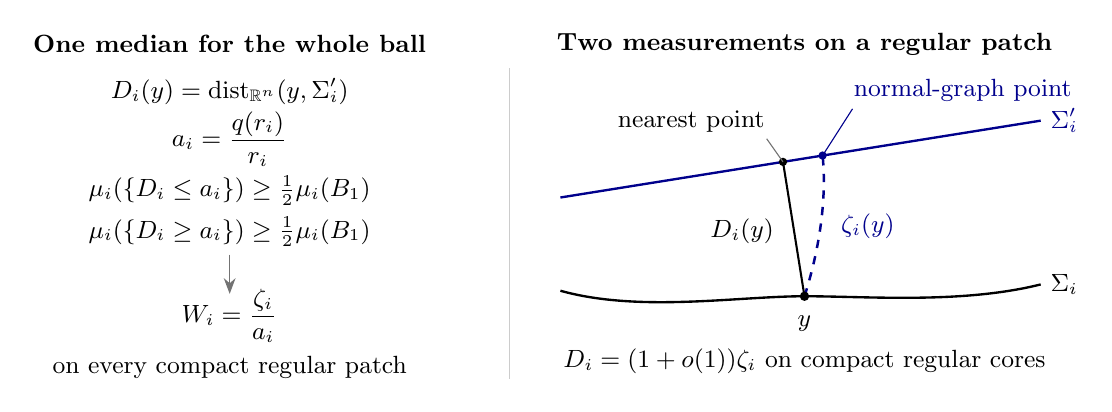
\begin{tikzpicture}[x=1cm,y=1cm,font=\small,
  every node/.style={inner sep=2pt},
  support/.style={line width=.85pt},
  measure/.style={line width=.75pt},
  graphheight/.style={line width=.9pt,dashed,blue!55!black}]
  \node[font=\small\bfseries] at (3.35,4.15)
    {One median for the whole ball};
  \node[font=\small\bfseries] at (10.65,4.15)
    {Two measurements on a regular patch};

  \node[align=center] at (3.35,3.55)
    {$D_i(y)=\dist_{\mathbb R^n}(y,\Sigma'_i)$};
  \node[align=center] at (3.35,2.95)
    {$\displaystyle a_i=\frac{q(r_i)}{r_i}$};
  \node[align=center] at (3.35,2.03)
    {$\mu_i(\{D_i\le a_i\})\ge\tfrac12\mu_i(B_1)$\\[4pt]
     $\mu_i(\{D_i\ge a_i\})\ge\tfrac12\mu_i(B_1)$};
  \draw[-{Stealth[length=2mm]},black!55] (3.35,1.48) -- (3.35,.98);
  \node[align=center] at (3.35,.47)
    {$\displaystyle W_i=\frac{\zeta_i}{a_i}$\\[4pt]
     on every compact regular patch};

  \draw[black!20] (6.9,-.1) -- (6.9,3.85);

  \draw[support] (7.55,1.02)
    .. controls (8.55,.74) and (9.8,.95) .. (10.65,.95)
    .. controls (11.45,.95) and (12.65,.85) .. (13.65,1.1);
  \node[anchor=west] at (13.7,1.1) {$\Sigma_i$};
  \draw[support,blue!55!black] (7.55,2.204) -- (13.65,3.18);
  \node[anchor=west,blue!55!black] at (13.7,3.18) {$\Sigma'_i$};

  \coordinate (y) at (10.65,.95);
  \coordinate (P) at (10.37699,2.65632);
  \coordinate (X) at (10.88,2.7368);
  \draw[measure] (y) -- (P)
    node[pos=.48,left=5pt] {$D_i(y)$};
  \draw[graphheight] (y)
    .. controls (10.82,1.48) and (10.94,2.14) .. (X)
    node[pos=.51,right=5pt] {$\zeta_i(y)$};
  \fill (y) circle (1.7pt);
  \node[below=5pt] at (y) {$y$};
  \fill (P) circle (1.5pt);
  \fill[blue!55!black] (X) circle (1.5pt);
  \node[anchor=south east] at (10.22,2.96) {nearest point};
  \draw[black!55,line width=.4pt] (10.17,2.95) -- (P);
  \node[anchor=south west,blue!55!black] at (11.2,3.35)
    {normal-graph point};
  \draw[blue!55!black,line width=.4pt] (11.26,3.33) -- (X);
  \node[align=center] at (10.65,.12)
    {$D_i=(1+o(1))\zeta_i$ on compact regular cores};
\end{tikzpicture}
\caption{A single distance median and its use on regular patches.
The curves are schematic regular cross-sections of the rescaled ordered
supports; no graph through the singular set is depicted.
The straight segment measures the ambient Euclidean nearest-support
distance $D_i(y)$, whereas the dashed segment is the normal exponential
segment of length $\zeta_i(y)$ in the rescaled earlier working metric
$g_i$. For $T_i(x)=x/r_i$, the measure
$\mu_i=r_i^{-k}(T_i)_\#\mu_{r_i}$ is the rescaling of the same
perimeter measure used to define $q(r_i)$, on all of $\Sigma_i\cap B_1$.
The number $a_i=q(r_i)/r_i$ is fixed using that whole measure before
regular patches are chosen. Both median
inequalities allow atoms, and every patch uses the same $a_i$.
The displayed relative comparison is uniform on each compact regular
core as $i\to\infty$.}
\label{fig:rpi:median-normalization}
\end{figure}


Choose a compact regular core inside $C\cap B_1$ whose omitted
area is less than one eighth of its total area, and enlarge it
slightly while keeping away from the singular set and sphere.
Such cores exist because those two sets have zero $k$-measure on
the cone. Graphical perimeter convergence makes the omitted area
less than one quarter for large $i$. Each median set therefore
retains positive measure on this fixed core.

\paragraph{Local bounds with the same normalization on every patch.}
Set $W_i=\zeta_i/a_i$. The lower median set and
\eqref{eq:rpi:distance-height} provide a point with $W_i\le2$ in
one of finitely many regular core patches. Choose that patch along
a subsequence. Weak Harnack for the nonnegative supersolution
$L_iW_i\le0$ gives a uniform local $L^p$ bound for some $p>0$,
before any bound for $F_i/a_i$ has been proved. To handle the
zero-order term, write
\[
 L_i=A_i^{ab}\partial_{ab}+B_i^a\partial_a+c_i
\]
and replace $c_i$ by $\min\{c_i,0\}$, obtaining $\widehat L_i$.
Since $W_i\ge0$, we still have $\widehat L_iW_i\le0$.
The usual weak Harnack inequality with nonpositive zero-order
coefficient applies with uniform constants on every fixed patch.

An $L^p$ bound on an overlap of fixed positive measure supplies a
bounded-value point for the next patch. Weak Harnack there propagates
the bound. Connectedness of $\operatorname{Reg}C$ gives finite
chains from the anchor patch to every fixed compact regular set.
Consequently
\begin{equation}\label{eq:rpi:median-local-lp}
 \|W_i\|_{L^p(K)}\le C_K
 \quad\hbox{for every }K\Subset\operatorname{Reg}C.
\end{equation}
The constants may grow with $K$. No uniform Harnack chain through
the singular set has been asserted.

\paragraph{Controlling the forcing before passing to a limit.}
The local $L^p$ bounds have been obtained without dividing a
right-side estimate by the possibly small number $a_i$. They now
let us control that quotient. In a ball
where $F_i\le-c\lambda_i$, solve
\[
 \widehat L_i\phi_i=-1,\qquad \phi_i|_{\partial B}=0.
\]
Uniform ellipticity, coefficient bounds, and the maximum principle
give $\phi_i\ge c_0>0$ on a smaller ball. Since
$\widehat L_i\zeta_i\le F_i$ and $\zeta_i\ge0$ on the boundary,
comparison gives
\[
 \zeta_i\ge c\lambda_i\phi_i.
\]
Combining this with \eqref{eq:rpi:median-local-lp} yields
$\lambda_i/a_i\le C_K$. The assumed upper bound for $|F_i|$
and a finite cover now give
\begin{equation}\label{eq:rpi:median-forcing-bound}
 \|F_i/a_i\|_{L^\infty(K)}\le C_K.
\end{equation}
The order is important: first weak Harnack, then the positive
Dirichlet comparison, and only then bounded-right-side elliptic
estimates.

The weak Harnack exponent need not exceed one. The local boundedness
estimate for the now bounded-right-side equation bounds the supremum
on an inner ball by the $L^2$ norm on a larger ball and the right-side
bound. Interpolate the $L^2$ norm between the bounded $L^p$ norm
and the larger-ball supremum, apply Young's inequality, and iterate
on nested radii to absorb that supremum. For each $i$ the preliminary
finite suprema exist by local regularity. This gives uniform local
$L^\infty$ bounds; interior elliptic estimates then give uniform
$W^{2,q}$ bounds for every finite $q$. One countable exhaustion and
one diagonal subsequence give a single function $W$, with local
$C^1$ convergence on all of $\operatorname{Reg}C$, satisfying
\begin{equation}\label{eq:rpi:median-limit}
 W\ge0,
 \qquad W\in W^{2,q}_{\rm loc}(\operatorname{Reg}C)
          \quad(q<\infty),
 \qquad (\Delta_C+|A_C|^2)W\le0.
\end{equation}
The upper median set also retains positive measure on the fixed
regular core. Equation~\eqref{eq:rpi:distance-height} gives points
there with $W_i\ge1/2$. Local uniform convergence makes $W$
nonzero. Since $\Delta_CW\le-|A_C|^2W\le0$, the strong maximum
principle and connectedness make $W>0$ throughout the regular part.
No separately normalized patch limits are used.

\paragraph{The infimum near the vertex.}
We have obtained one positive limit on the entire regular part. The
record-scale choice now gives information on its behavior near the
vertex without changing its normalization or taking new patchwise
limits.

Fix $0<\rho\le1$. The lower median set in $\Sigma_i\cap B_\rho$
has half its area and, by \eqref{eq:rpi:median-record}, normalized
ambient distance at most $2\rho$. Choose a compact regular core
in $C\cap B_\rho$ omitting less than one quarter of its area.
Perimeter convergence and \eqref{eq:rpi:distance-height} give a
point in this core with $W_i\le3\rho$ for large $i$. The already
chosen local uniform convergence applies to this core. Thus the
same limit satisfies
\begin{equation}\label{eq:rpi:median-small-infimum}
 \inf_{\operatorname{Reg}C\cap B_\rho}W\le3\rho.
\end{equation}
It is enough to use a countable sequence of $\rho\downarrow0$.
The constant $3$ does not depend on the core or on $\rho$: for
each fixed radius the relative error in
\eqref{eq:rpi:distance-height} tends to zero before this limit is
taken. Therefore the infimum of $W$ in every ball about the vertex
is zero. Its essential infimum there is also zero, since every
small regular value has a neighborhood of positive perimeter measure
with comparably small values.

\paragraph{A bounded supersolution across the singular set.}
To apply a mean-value inequality on the whole minimizing cone, we
need a Sobolev supersolution across its singular set. First discard
the nonnegative Jacobi potential, obtaining $\Delta_CW\le0$, and
then set $h=\min\{W,1\}$. Approximation by increasing concave truncations
shows that $h$ is a bounded positive weak \emph{Laplace}
supersolution on the regular part. It need not be a Jacobi
supersolution. For a regular-part cutoff $\eta$, use the nonnegative
test $\eta^2(1-h)$ to obtain
\[
 \int\eta^2|\nabla_C h|^2
 \le2\int\eta(1-h)|\nabla_C h||\nabla_C\eta|,
\]
and hence
\begin{equation}\label{eq:rpi:truncation-energy}
 \int\eta^2|\nabla_C h|^2
       \le4\int|\nabla_C\eta|^2.
\end{equation}

The singular set has zero tangential two-capacity on compact regions.
Indeed, cover the relevant compact singular set by finitely many balls
$B_{\rho_j}(x_j)$, with centers on that set, maximum radius tending
to zero, and $\sum_j\rho_j^{k-2}\to0$. This is possible because
its dimension is at most $k-7$. Let $\theta_j$ vanish on the ball,
equal one off its double, and satisfy $|D\theta_j|\le C/\rho_j$.
Put $\chi=\min_j\theta_j$. Almost everywhere its gradient is one
of the active gradients, so local area growth gives
\begin{equation}\label{eq:rpi:cone-capacity}
 \int_C|\nabla_C\chi|^2
 \le\sum_j\int_{C\cap B_{2\rho_j}(x_j)}|\nabla_C\theta_j|^2
 \le C\sum_j\rho_j^{k-2}\longrightarrow0.
\end{equation}
There is no overlap-count factor. These cutoffs vanish near the
whole relevant singular set and converge to one on the regular part.

Use $\eta=\psi\chi$ in \eqref{eq:rpi:truncation-energy}, where
$\psi$ is a fixed compact spatial cutoff. Fatou's lemma gives
locally finite Dirichlet energy for $h$ across the singular set.
Moreover, $\psi h\chi\to\psi h$ in the local surface
$W^{1,2}$ norm: the term $h\nabla_C\chi$ tends to zero by
boundedness and \eqref{eq:rpi:cone-capacity}, while the omitted
$\nabla_C h$ term tends to zero by absolute continuity of its
now finite energy. Thus $h$ genuinely extends as a local Sobolev
function on the whole minimizing boundary; its values on the
measure-zero singular set are immaterial.

For a nonnegative ambient smooth compactly supported test function
$\varphi$, insert $\varphi\chi$ into the regular-part supersolution
inequality. The cutoff error is bounded by
\[
 \|\varphi\|_\infty
 \|\nabla_C h\|_{L^2(\supp\varphi)}
 \|\nabla_C\chi\|_2\longrightarrow0.
\]
The other term converges by dominated convergence. Hence
\[
 \int_C\langle\nabla_C h,\nabla_C\varphi\rangle\ge0
\]
for tests meeting the singular set as well.

\paragraph{The mean-value contradiction.}
The bounded function $h$ is now a positive weak Laplace supersolution
on the whole minimizing boundary, with locally finite energy and zero
essential infimum in every ball about the vertex. These are the
conditions needed for the minimizing-boundary weak Harnack theorem
of Bombieri--Giusti \cite{BombieriGiusti1972Harnack}; the precise
form needed here is stated in
\cite[Theorem~3.1, p.~11]{DeSilvaJerison2011Gradient}.
For an area-minimizing hypersurface in $B_R$ and a positive weak
Laplace supersolution, a normalized $L^p$ mean on $B_r$ is bounded
by its infimum on $B_r$ when $r\le\beta R$ and
$0<p<k/(k-2)$. The constants depend only on dimension and $p$.
This is an extrinsic estimate on the minimizing boundary, not an
assertion that regular-patch Harnack chains have uniform constants
through cone singularities.

Apply it to $h+\epsilon$ on the cone, with fixed concentric balls
and, for example, $p=1$. Choose the smaller ball to contain a regular
open subset on which $h>0$; the cone and the same $h$ are defined
on any required larger ball. Its conclusion is
\[
 \frac{1}{\mathcal H^k(C\cap B_r)}
       \int_{C\cap B_r}(h+\epsilon)
 \le C\operatorname*{ess\,inf}_{C\cap B_r}(h+\epsilon).
\]
The essential infimum of $h$ is zero by
\eqref{eq:rpi:median-small-infimum}. Sending $\epsilon\downarrow0$
would make the positive integral on the left zero, a contradiction.
This proves separation. No growth selection at infinity or limiting
truncation level is needed.
\end{proof}

\subsection{The graph equation for the two deformations}
\label{sec:rpi:separation-application}

It remains to verify the separation proposition for the flow and for
the prescribed-curvature enclosure. Both use the same graph equation;
the difference is a small zero-order term in the latter problem. We
derive the equation using the end-pointing normal throughout.

Normalize the earlier working metric $g$ at the contact point to be Euclidean, write $g_i$
for its rescaling at radius $r_i$, and use $g_i$-unit normals and
$g_i$-normal exponential graphs throughout. For this calculation assume uniform $C^{3,\alpha}$ bounds for the
extended metrics and graphs on a larger regular cone patch.
Lemma~\ref{lem:rpi:simultaneous-regularity} supplies them for flow
slices; the candidate construction below will supply them in the
second application.
Continuity of the original metric gives uniform convergence to its
contact-point value. Apply bounded graph-domain extension operators
to its difference from that constant metric; these preserve uniform
convergence. Interpolation then gives $g_i\to\delta$ in $C^2$
on a smaller patch. The graph bounds similarly give the $C^2$
convergence needed below. A mere $C^{1,\alpha}$ metric bound would
not justify convergence of the Ricci term.

The linearization of $H=\divg\nu$ at the earlier minimal graph is
$-J_i$, where
\[
 J_i=\Delta_{\Sigma_i,g_i}+|A_i|_{g_i}^2
                          +\Ric_{g_i}(\nu_i,\nu_i).
\]
Integrating the derivative of the mean-curvature graph operator from
height zero to $\zeta_i$ writes its nonlinear remainder as
\[
 Q_i\zeta_i
   =Q_i^{ab}\partial_{ab}\zeta_i
      +Q_i^a\partial_a\zeta_i+Q_i^0\zeta_i,
\]
with coefficients tending locally to zero. Let the later metric be
$g'_i=U_i^{4/d}g_i$, and let its prescribed end-oriented curvature
be $f_i(y)=r_i f(\eta_i(y))$, where $\eta_i(y)=p+r_i y$.
The conformal formula gives the exact equation
\begin{equation}\label{eq:rpi:separation-graph-equation}
 (J_i-Q_i)\zeta_i=F_i-U_i^{2/d}f_i,
 \qquad F_i=\frac{2k}{d}U_i^{-1}
                         \partial_{\nu'_i}^{g_i}U_i.
\end{equation}
For flow slices $f=0$ and $U_i$ is the rescaled ratio $u_t/u_s$.
Equations~\eqref{eq:rpi:relative-integrands}--
\eqref{eq:rpi:relative-forcing} give the required two-sided relative
bound for $F_i$.

\subsection{Separation of flow slices}
\label{sec:rpi:flow-slice-separation}

Fix $0\le s<t$. We prove that the two closed supports are disjoint.
Suppose $p\in\Sigma_s\cap\Sigma_t$ is regular
for at least one frontier. The simultaneous regular-neighborhood
lemma makes both graphs regular there. Nesting puts $p$ on every
intermediate frontier: an interior point of an intermediate conductor
would be interior to $K_t$. These ordered graphs have a common
tangent plane and the same end-oriented normal. Their velocities
vanish at $p$, so $u_t(p)=u_s(p)$.

For each $\sigma\in[s,t]$, the function
$z_\sigma=-v_\sigma/u_s$ is positive and $g_s$-harmonic on its
own exterior $E_\sigma$, vanishes at $p$, and has strictly positive
derivative in the common $g_s$-unit normal direction. Uniform
boundary $C^1$ bounds and the positive lower bound for $u_s$ give
an integrable bound for these measurable derivatives. The uniform
$C^2$ common-tangent graph charts provide a single short outward
normal segment in $E_t$, hence in every $E_\sigma$; all exterior
difference quotients can be taken there. Thus, with $q=u_t/u_s$,
Equation~\eqref{eq:rpi:relative-integral} gives
\[
 \partial_\nu q(p)
       =-\int_s^t\partial_\nu z_\sigma(p)\,d\sigma<0.
\]
Extend the later metric from its exterior as a $C^1$ metric. Its
first jet at $p$ is determined by that one-sided metric, and the
earlier metric has the matching one-sided jet. The conformal
mean-curvature formula at this point gives
\[
 H_{\Sigma_s}^{g_t}(p)
 =q(p)^{-2/d}\left(H_{\Sigma_s}^{g_s}(p)
                +\frac{2k}{d}q(p)^{-1}\partial_\nu q(p)\right)<0.
\]
The earlier curvature is zero, including at $s=0$. The later graph
has zero curvature in the same extension metric. Since $K_s\subset K_t$,
the tangent graph comparison gives
$H_{\Sigma_t}^{g_t}(p)\le H_{\Sigma_s}^{g_t}(p)<0$, a contradiction.
Only the common exterior first jets were used; the ratio need not be
constant on the later frontier or harmonic throughout $E_s$.
Thus regular contact is impossible. At any remaining contact, the
power almost-minimizing estimates and density bounds give the common
minimizing-cone limits used in
Proposition~\ref{prop:rpi:singular-separation}. The regular-patch
bootstrap, relative harmonic derivative estimate, and graph equation
verify its remaining hypotheses. The proposition excludes singular
contact as well, proving $\Sigma_s\cap\Sigma_t=\varnothing$.

\subsection{The prescribed-curvature enclosure before detachment}
\label{sec:rpi:perturbed-candidate}

We now build the enclosing frontier needed for the mass--capacity
comparison. The construction applies both to a flow slice and to the
original smooth ambient metric in the approximation argument. In
either case, the initial frontier is locally perimeter minimizing;
its enclosing candidate must be understood before detachment is known.

Let $K$ be a compact canonical closed filled set with nonempty
frontier $\Sigma$ and connected open end exterior $E$. Work in either
of the following settings:
\begin{enumerate}
\item $K=K_s$ is a flow conductor and $h=b^2g_s$ for a fixed
      constant $b>0$;
\item $h$ is smooth through $\Sigma$ and on $E$, and $K$ is
      locally perimeter minimizing in $h$ on a neighborhood of
      $\Sigma$. The exterior has one coordinate end and compact
      complement, with $h_{ab}=a_0^2\delta_{ab}+O_2(r^{-\tau_0})$
      for constants $a_0,\tau_0>0$.
\end{enumerate}
In the second case extend $h$ smoothly a short distance behind the
frontier and, if needed, use the buried-boundary construction already
described. No outermost property of $K$ is required. In both settings
$K$ is locally minimizing in its continuous metric $h$: for a flow
slice this is Lemma~\ref{lem:rpi:flow-construction}, and in the
smooth setting it is the stated hypothesis. The density and minimizing
cone conclusions follow from the same local comparison.

Let $u$ be a positive $h$-harmonic function on $E$, continuous up to
$\Sigma$, with $u=1$ there, $u<1$ in $E$, and $u\to\ell\in(0,1)$
at infinity. Extend it by one on $K$ and set $h'=u^{4/d}h$.
Assume on the coordinate end that
$h'_{ab}=a^2\delta_{ab}+O_2(r^{-\tau})$, where $a,\tau>0$.
This differentiated decay will confine the candidate inside a fixed
coordinate sphere.

The extended perturbation has the H\"older modulus needed for the
weighted perimeter comparison. To see this directly in the flow
case, the conformal Laplacian identity makes
\[
 z=u_s(1-u)
\]
a bounded positive $g_0$-harmonic function on $E_s$, continuous with
zero frontier value and end value
$c=e^{-s}(1-\ell)>0$. Let $q_{K_s}$ be the escape potential for
$g_0$, constructed in the proof of
Lemma~\ref{lem:rpi:flow-construction}. Bounded continuous Dirichlet
uniqueness gives $z=cq_{K_s}$. The already proved H\"older modulus
of $q_{K_s}$ and the positive H\"older factor $u_s$ therefore give
\[
 u=1-\frac{cq_{K_s}}{u_s}
\]
with a H\"older extension across $\Sigma$. For a smooth initial
metric, use the same background capacitary construction with $h$ in
place of $g_0$. Local minimizing density gives its boundary
contraction estimate, and uniqueness gives
$1-u=(1-\ell)q_K$. Thus $h'$ is a positive H\"older metric in
both cases, before the candidate is constructed.

Choose a smooth ambient function $h_0$ that is zero on $K$, positive
on $E$, and integrable in $h'$. A locally finite partition of unity
in $E$, with coefficients decreasing sufficiently rapidly, makes its
zero extension smooth and its integral finite. Its first derivative
vanishes along $\Sigma$; in particular, on compact sets,
$|h_0(x)|\le C\operatorname{dist}(x,\Sigma)$.

For $\delta>0$ chosen below, the candidate $K'$ minimizes
\[
 \mathcal F(L)=P_{h'}(L)
       +\delta\int_{L\setminus K}h_0\,dV_{h'}
\]
among all compact finite-perimeter supersets of $K$ in the ambient
manifold. The added region $L\setminus K$ need not stay a positive
distance from the original frontier. The parameters, forcing, and its derivatives are
fixed here. To fix the sign, a normal variation $\varphi\nu$ of the candidate
frontier has first variation
\[
 D\mathcal F[\varphi\nu]
   =\int_{\partial K'}(H_\nu+\delta h_0)\varphi\,dA_{h'}.
\]
Its prescribed end-oriented curvature is therefore $H=-\delta h_0$.
The function $h_0$ vanishes on the original filled side; its value on
the candidate frontier has not been prescribed to be zero.

\paragraph{Existence, compact support, and a connected end exterior.}
On the asymptotically flat end, $h'$ is smooth and approaches a positive constant multiple
of the Euclidean metric, with the corresponding differentiated decay.
Choose $R_*$ enclosing $K$ so that every coordinate sphere beyond
$R_*$ has strictly positive outward mean curvature in $h'$. This
choice precedes that of $\delta$. First minimize $\mathcal F$ over
all finite-perimeter supersets of $K$ in a coordinate truncation
$B_Q$, including the compact core, with $Q>R_*$.
The competitor $K$ gives a perimeter bound. BV compactness, lower
semicontinuity for the positive continuous perimeter weight, and
$L^1$ convergence of the bounded volume density on $B_Q$ give a
minimizer. If $X$ is the outward $h'$-unit normal to the coordinate
spheres, the divergence formula gives, for almost every $r>R_*$,
\[
 P_{h'}(L\cap B_r)
 \le P_{h'}(L)
       -\int_{L\setminus B_r}\operatorname{div}_{h'}X\,dV_{h'}.
\]
The divergence is positive. Clipping also decreases the nonnegative
volume term, strictly decreasing $\mathcal F$ whenever the removed
tail has positive volume. The minimizer is therefore supported in
$B_{R_*}$, independently of $Q$ and $\delta$. Clipping an arbitrary
compact competitor into this same ball proves global minimality,
with no artificial outer constraint remaining.

To ensure a filled enclosure, choose $\delta>0$ sufficiently small
after fixing $h'$ and $R_*$. Compact-support isoperimetry gives
\[
 \Vol_{h'}(U)^{k/n}\le C_{\rm iso}P_{h'}(U)
\]
for sets $U\subset B_{R_*}$ disjoint from the buried collar. Such
sets have zero trace on a slightly larger smooth truncation, so
this is the absolute inequality. Require
\[
 \delta\|h_0\|_{L^\infty(B_{R_*})}
 C_{\rm iso}\Vol_{h'}(B_{R_*})^{1/n}<1.
\]
In a larger truncation $B_{Q_2}$, decompose $B_{Q_2}\setminus L$
into its finite-perimeter components. Exactly one contains the
connected outer annulus; let $U$ be the union of the others.
Perimeter additivity, with cancellation of the outer sphere, shows
that filling $U$ removes its perimeter. Consequently
\[
 \mathcal F(L\cup U)-\mathcal F(L)
 =-P_{h'}(U)+\delta\int_Uh_0\,dV_{h'}<0
\]
unless $U$ has zero volume. This contradicts minimality. The selected
minimizer is thus filled and has connected end exterior, while
retaining minimality against all finite-perimeter enclosing
competitors. No positive lower bound on $\delta$ is needed.

\paragraph{Local variations across the original frontier.}
The existence argument has produced a global enclosing minimizer.
To obtain its graph equation near possible contact, we remove the
enclosure constraint for local variations. Let $L\triangle K'$ be
compactly supported in a sufficiently small variation ball. Since
$h'=h$ on $K$, the local minimizing property of $K$ gives
\[
 P_{h'}(L\cap K)\ge P_{h'}(K),\qquad
 P_{h'}(L\cup K)\le P_{h'}(L),
\]
where the second inequality is perimeter submodularity and all
comparisons are localized to that ball. This argument uses only local
minimality of the given $K$; it does not replace it by an outermost
hull.
The volume term is modular under union and intersection, and its
density is zero on $K$. In particular its value on $L\cup K$
equals its value on $L$. Constrained minimality of $K'$ against
$L\cup K$ therefore gives $\mathcal F(K')\le\mathcal F(L)$.
This proves local unconstrained minimality. Its comparison with the
smooth reference metric yields the uniform almost-minimizing estimate
from the H\"older weight, with an additional error at most $Cr^n$
from the bounded volume forcing.
The canonical density representative removes null cracks; for these
almost-minimizing sets, absence of bounded complementary BV components
therefore gives the connected open end exterior asserted above.

\paragraph{Uniform graph estimates before separation.}
At a hypothetical common tangent-cone patch, the local comparison just
proved and one-sided small-excess regularity give uniform
$C^{1,\theta}$ candidate graphs.
For a flow conductor, the original graph and its one-sided metric
have the all-order bounds in
Lemma~\ref{lem:rpi:simultaneous-regularity}. In the smooth initial
setting, the rescaled smooth metric has uniform bounds and the
minimal graph equation supplies the same regular-patch estimates.
Harmonic boundary estimates for $u$, whose original graphical
boundary value is constant, give all fixed finite orders on smaller
patches. The metric $h'$ consequently has controlled extensions
from the original exterior.

For the first graph equation, extend $1-u$ oddly through the original
regular graph. It is negative on the filled side, so the corresponding
$C^{1,\alpha}$ extension of $u$ is at least one there and dominates
its original extension. In the smooth initial setting multiply this
factor into the smooth metric $h$. In the flow setting, first use the
dominating extension of $b^2g_s$ from
Lemma~\ref{lem:rpi:simultaneous-regularity}, and multiply the two
extended conformal factors. After shrinking the patch the resulting
metric is positive, dominates $h'$, and agrees with it on the original
exterior, hence on the candidate graph.
The forcing density is unchanged where $h_0$ is nonzero, because
that region lies in the original exterior; on $K$ it is zero in
both metrics. Thus $K'$ remains a local minimizer of the same
perimeter-plus-volume functional in this regular extension metric.
Its weak Euler equation is exactly
\[
 H_{\nu}^{h'}=-\delta h_0.
\]

The uniformly elliptic prescribed-mean-curvature graph equation
improves the candidate to $C^{2,\alpha}$. The original metric and
harmonic perturbation have the higher-order coefficient extensions
already established, so elliptic bootstrapping gives every fixed
higher-order candidate estimate on smaller patches. After the first
equation is established, these extensions need only match the
one-sided boundary jets; domination is no longer required.
Under a radius-$r_i$ blow-up the forcing is
$r_i(-\delta h_0)(r_i y)$, with uniform local coefficient bounds
of every fixed order. The candidate's estimates therefore precede
and do not assume singular separation.

These estimates already exclude contact at a regular point. At contact with
the original graph, $h_0=0$, whereas the strict harmonic conformal
derivative makes the original graph have strictly negative
end-oriented mean curvature in $h'$. The candidate equation has
zero curvature there. Ordered graph comparison forbids contact.
If only one frontier was initially known to be regular there, the
one-sided regular-neighborhood argument first makes the other
regular. This excludes regular contact only; singular contact is
the separate issue addressed next.

\paragraph{The candidate graph equation and singular detachment.}
Apply Equation~\eqref{eq:rpi:separation-graph-equation} with earlier
metric $g=h$, later metric $h'=u^{4/d}h$, and prescribed curvature
$f=-\delta h_0$. Since $f$ is smooth and zero on $K$, it satisfies
$|f(x)|\le C\operatorname{dist}(x,\Sigma)$. The original distance
from a point at rescaled graph height $\zeta_i$ to $\Sigma$ is at
most $Cr_i\zeta_i$, and therefore
\[
 |U_i^{2/d}f_i|\le Cr_i^2\zeta_i.
\]
Put $b_i=U_i^{2/d}f_i/\zeta_i$ and absorb this term into the operator:
\[
 L_i=J_i-Q_i+b_i,\qquad |b_i|\le Cr_i^2,
 \qquad L_i\zeta_i=F_i\le0.
\]
The coefficient also has a uniform H\"older bound. Indeed, $f$ vanishes
on the earlier graph, so the fundamental theorem of calculus along
the normal graph segment expresses $f_i/\zeta_i$ as $r_i^2$ times
an average of first derivatives of $f$. The smooth forcing and the
uniform graph and metric bounds control that average in the fixed
regular-patch coordinates. Thus $b_i\to0$ and $L_i\to J_C$ with
the coefficient control required by
Proposition~\ref{prop:rpi:singular-separation}.

The sign of $f$ is not needed in this absorption. The strictly
negative right side instead comes from the harmonic conformal factor:
Lemma~\ref{lem:rpi:relative-harmonic}, applied to $1-u>0$, gives the
patchwise two-sided relative bounds for $F_i$. All parameters have
remained fixed during this argument.

\begin{corollary}[Detachment of slices and perturbed enclosures]
\label{cor:rpi:flow-detachment}
For any fixed $0\le s<t$, the conformal-flow frontiers
$\Sigma_s$ and $\Sigma_t$ are disjoint as closed perimeter supports.
For either the flow or smooth initial exterior in
Section~\ref{sec:rpi:perturbed-candidate}, let $u$ satisfy the
harmonic, boundary, strictness, and end hypotheses stated there. For the forcing and
sufficiently small fixed $\delta>0$ constructed there, the
perimeter-plus-volume minimizer is disjoint from the original
frontier, including its singular set. Each fixed pair of these
compact supports has positive distance.
\end{corollary}

\begin{proof}
The flow assertion was proved in
Section~\ref{sec:rpi:flow-slice-separation}. For the perturbed
enclosure, the preceding regular comparison excludes regular
contact. The power almost-minimizing estimate, the regular-patch
metric and graph bounds, and the displayed forcing equation verify
Proposition~\ref{prop:rpi:singular-separation}, which excludes the
remaining singular contact. Compactness of each pair of supports
then gives positive distance. The constants and the resulting
distance may depend on the fixed time pair or perturbation parameter.
\end{proof}

\section{Capacity and one-sided smoothing}
\label{sec:rpi:orientation}

The mass decrease in conformal flow is controlled by the difference
between ADM mass and capacity. To show that this difference is
nonnegative, we first move a possibly singular frontier toward the
asymptotic end and smooth it with a definite mean-curvature sign.
The capacity does not decrease under this operation. We can then apply a
smooth mass--capacity inequality, proved below from positive mass.

Throughout this section $n\ge3$, $\omega=|S^{n-1}|$, and $\nu$
denotes the normal from a compact removed region toward the
asymptotically flat end. For a frontier $\Sigma$ we use
$H_\nu=\divg_\Sigma\nu$.
For a smooth compact conductor with exterior $(E,h)$, normalize
capacity by
\begin{equation}\label{eq:rpi:capacity}
 \mathfrak c(\Sigma,h)=\frac1{(n-2)\omega}
             \int_E|dw|_h^2\,dV_h,
 \qquad \Delta_h w=0,\quad w|_\Sigma=1,\quad w\to0.
\end{equation}
Equivalently, this is the normalized infimum of Dirichlet energy
among smooth compactly supported trial functions equal to one in a
neighborhood of the conductor. The same variational definition
applies to a nonsmooth compact conductor.
If one conductor contains another, its admissible class is smaller,
so its capacity is no smaller.

\subsection{A harmonic perturbation and its detached enclosure}

We first construct a boundary with a strict curvature sign; the next
subsection will smooth it. Let $(E,g)$ be a flow-slice exterior or
a smooth-ambient initial exterior as in Theorem~\ref{thm:rpi},
and assume its frontier is
nonempty. Let $w$ be its capacitary potential and put $v=w-1$.
The strong maximum principle gives
$-1<v<0$ in the open exterior, while $v=0$ on the frontier.
For $0<\varepsilon<1$ set
\[
 u_\varepsilon=\frac{1+\varepsilon v}{1-\varepsilon},\qquad
 \widetilde g_\varepsilon=u_\varepsilon^{4/(n-2)}g.
\]
Harmonicity gives
$R_{\widetilde g_\varepsilon}=u_\varepsilon^{-4/(n-2)}R_g\ge0$
on the exterior.
The perturbing factor tends to one at infinity, preserving the end
normalization of $g$. To apply the detachment
corollary, whose harmonic factor has boundary value one, express
the same metric as
\[
 g^{\rm base}_\varepsilon=(1-\varepsilon)^{-4/(n-2)}g,
 \qquad \widehat u_\varepsilon=1+\varepsilon v,
 \qquad
 \widetilde g_\varepsilon
   =\widehat u_\varepsilon^{4/(n-2)}g^{\rm base}_\varepsilon.
\]
Then $\widehat u_\varepsilon=1$ on the frontier and
$1-\varepsilon<\widehat u_\varepsilon<1$ in $E$.
If $g^{\rm base}_\varepsilon=\kappa^2g$, then
\[
 \Delta_{g^{\rm base}_\varepsilon}=\kappa^{-2}\Delta_g,
 \qquad \nu_{g^{\rm base}_\varepsilon}=\kappa^{-1}\nu_g,
 \qquad H^{g^{\rm base}_\varepsilon}=\kappa^{-1}H^g.
\]
Constant scaling preserves harmonicity, minimality and the local
almost-minimizing hypotheses, with changed constants. It also preserves
the signs and relative bounds of normal derivatives. At regular
boundary points the Hopf derivative of $\widehat u_\varepsilon$
in the direction $\nu$ is strictly negative, so the conformal
mean-curvature formula makes the original frontier a strict inner
barrier in $\widetilde g_\varepsilon$.

Apply the prescribed-curvature construction of
Section~\ref{sec:rpi:perturbed-candidate} to this fixed perturbation,
using its smooth forcing $h_0$, zero on the original filled side and
positive in its exterior. With the sufficiently small fixed volume
parameter $\delta>0$, Corollary~\ref{cor:rpi:flow-detachment} separates
the candidate from the full original frontier. Denote its connected
end exterior by $E'$. In the perturbed metric
$\widetilde g_\varepsilon$, a variation of its filled side by
$\varphi\nu$ has first variation
\begin{equation}\label{eq:rpi:first-variation}
 D\mathcal F[\varphi\nu]
       =\int_{\partial E'}(H_\nu+\delta h_0)\varphi\,dA,
\end{equation}
and therefore its regular frontier satisfies
\begin{equation}\label{eq:rpi:corrected-sign}
 H_\nu=-\delta h_0\le-\gamma<0.
\end{equation}
Here $\gamma>0$ exists because the entire detached frontier is a
compact subset of the original exterior, where $h_0>0$.
The perturbed metric is smooth on its neighborhood. All perturbation and
forcing parameters remain fixed through separation and smoothing;
no curvature or separation bound uniform in $\varepsilon$ is needed.

Strictness matters: if $u\equiv1$, the forcing is zero, and the
original frontier is outer minimizing and minimal, the original
exterior remains a minimizing competitor. Separation cannot follow
from $u\le1$ alone.

\begin{remark}[Orientation and the literature]
On the Euclidean exterior $r\ge a$, our convention gives
\[
 H_\nu=(n-1)/a>0,\qquad m_{\rm ADM}=0,\qquad
 w=(a/r)^{n-2},\qquad\mathfrak c=a^{n-2}>0.
\]
The smooth mass--capacity inequality therefore requires the
nonpositive sign with this normal. This example distinguishes the
statement here from the positive-$H_\nu$ inequality in
\cite[Lemma~3.11]{BiZhu2026}, which is version~1. Version~2 uses
the outward normal of the exterior in its Lemma~3.10, hence the
opposite normal at the inner frontier. Its Corollary~2.37 includes
the strict harmonic-factor hypothesis, and its Lemma~3.7 includes
the base-metric normalization \cite{BiZhu2026v2}.
\end{remark}

\subsection{Smooth frontiers with the required sign}
\label{sec:rpi:smoothing}

The distance-offset construction in
\cite[Section~3 and Proposition~2.6]{BiZhuSmoothing2026},
arXiv:2605.12403v2, supplies the geometric strategy for the next
proposition. The conclusion needed for capacity is conductor inclusion and a
mean-curvature bound. We prove precisely this conclusion using
Rifford's minimum-family theorem locally and a final smoothing of
transverse graphs. Boundary-area convergence is not needed.

\begin{proposition}[One-sided smoothing in a shrinking collar]
\label{prop:rpi:one-sided-smoothing}
Let $\Omega$ be an open subset of a smooth Riemannian manifold with
compact full boundary $\Sigma$. Assume that the metric is smooth on
an ambient neighborhood of $\Sigma$. Let $\Lambda\subset\Sigma$
consist of the points touched by a geodesic ball contained in $\Omega$.
Suppose that $\Lambda$ is a smooth embedded hypersurface, locally
bounds $\Omega$ on its accessible side, and has mean curvature at
least $\gamma>0$ for the normal pointing out of $\Omega$.

For every $\varepsilon>0$, there is an open set
$\Omega_\varepsilon\subset\Omega$ with smooth compact boundary such
that
\[
 \Omega\setminus\Omega_\varepsilon
 \subset\{x\in\Omega:\dist(x,\Sigma)<\varepsilon\},
 \qquad
 H_{\mathrm{out},\Omega_\varepsilon}\ge\gamma-\varepsilon.
\]
\end{proposition}

\begin{proof}
If $\Sigma$ is empty, take $\Omega_\varepsilon=\Omega$.
Otherwise we first choose a regular distance level, then take a short offset
of its superlevel, and finally smooth the resulting $C^{1,1}$
hypersurface. The offset controls curvature; the final smoothing
loses an arbitrarily small amount of that bound.

Write $\rho(x)=\dist(x,\Sigma)$ on $\Omega$. All distances and
geodesics below are taken in the ambient metric. Choose a relatively
compact ambient neighborhood of $\Sigma$ and a smaller compact safety
neighborhood. Fix $r_*>0$ much smaller than the distance separating
their boundaries and the injectivity radii on the larger compact
neighborhood. Short paths used in the proof then stay in the region
of controlled smooth geometry, and the squared-distance functions
used for pairs less than $4r_*$ apart are smooth. No completeness of
an auxiliary ambient extension is needed.

\paragraph{Regular distance levels.}
If $0<\rho(x)<r_*$, every nearest point of $\Sigma$ to $x$ belongs to
$\Lambda$. Indeed, a shortest segment from $x$ to the full boundary
stays in $\Omega$ until its endpoint, and a shorter terminal subsegment
supplies an interior tangent ball there. The nearest-point set is
compact. It therefore lies in the interior of a compact smooth
hypersurface patch $Q\subset\Lambda$ with smooth boundary. Choose
$Q$ sufficiently close to that set that
$\dist(y,q)^2$ is smooth for $q\in Q$ and $y$ near $x$.

Because $\Lambda$ is embedded, there is an ambient open set
$\mathcal V$ containing the nearest-point set with
$\mathcal V\cap\Lambda\subset\operatorname{int}_{\Lambda}Q$.
After shrinking the neighborhood of $x$, every nearest point to each
such $y$ lies in $\mathcal V$. Otherwise, compactness of
$\Sigma\setminus\mathcal V$ would give a nearest point of $x$
outside $\mathcal V$. These nearby nearest points belong to
$\Lambda$ by the preceding tangent-ball argument, and hence lie
in the interior of $Q$. Thus
\[
 \rho(y)^2=\min_{q\in Q}\dist(y,q)^2
\]
on an open neighborhood of $x$. Apply
\cite[Theorem~3 and the compact-parameter-with-boundary extension
in the proof of Theorem~1]{Rifford2004}. A countable family of these
neighborhoods covers the small distance collar, so the critical
values of $\rho^2$ form a null set. On each compact interval of
positive distances, the square-root map is Lipschitz and
$\partial_C(\rho^2)=2\rho\,\partial_C\rho$, where $\partial_C$
denotes the Clarke differential. Thus the positive critical values
of $\rho$ also form a null set. Choose $s_i\downarrow0$ such that
\[
 0\notin\partial_C\rho(x)\qquad\text{whenever }\rho(x)=s_i.
\]
The compact parameter patch is the reason this theorem applies even
though the accessible locus $\Lambda$ need not be closed.

\paragraph{Positive reach of the superlevels.}
The distance function is locally semiconcave away from $\Sigma$.
To obtain smooth upper supports, take a minimizing segment from
$\Sigma$ to a point of the collar and retain a short terminal piece.
Distance from its earlier endpoint, plus the length of the preceding
piece, is a smooth upper support near the terminal point. The local
Hessian comparison estimate gives a uniform upper Hessian bound on
a sufficiently small fixed ball. Consequently, in a geodesic
coordinate ball,
\begin{equation}\label{eq:rpi:smoothing-semiconcavity}
 \rho(y)\le\rho(x)+\langle p,\log_x y\rangle
                  +C\dist(x,y)^2
 \qquad(p\in\partial_C\rho(x)).
\end{equation}
Here the superdifferential of the semiconcave function agrees with its
Clarke differential.

We include the regular-superlevel implication underlying the
positive-reach criterion associated with \cite{Bangert1982}.
At a point of a regular level, let
$\mathcal K=\partial_C\rho(x)$. This is a compact convex set not
containing zero. Separation gives a direction $v_0$ such that
$\langle p,v_0\rangle>0$ for every $p\in\mathcal K$. The directional
derivative of a semiconcave function is
$\min_{p\in\mathcal K}\langle p,v\rangle$. Every direction for which
this minimum is positive therefore enters the superlevel. Separation
of convex cones implies that the polar of its contingent tangent
cone, and in particular each proximal outward normal, is contained
in $-\operatorname{cone}(\mathcal K)$. Since $\mathcal K$ is convex,
each unit proximal outward normal can be written
$\mathbf n=-p/|p|$ with $p\in\mathcal K$.

Compactness of the level and upper semicontinuity of the
superdifferential give a uniform lower bound $|p|\ge\eta>0$ there.
For a nearby point $y$ of the superlevel,
Equation~\eqref{eq:rpi:smoothing-semiconcavity} yields
\[
 \langle\mathbf n,\log_x y\rangle
       \le\frac C\eta\dist(x,y)^2.
\]
This gives uniqueness of sufficiently nearby nearest-point
projection. Indeed, suppose that $z$ had two distinct nearest
points $x,y$, at the same distance $a$. In a sufficiently small
bounded-geometry ball, the Taylor expansion of squared distance
from $z$ gives
\[
 0=\dist(z,y)^2-\dist(z,x)^2
 \ge-2a\langle\mathbf n,\log_x y\rangle
                         +\frac12\dist(x,y)^2.
\]
For $a<\eta/(4C)$ this contradicts the preceding bound. Enlarging
the constants slightly covers the curvature terms. Compactness
excludes distant distinct nearest points when $a$ is small and
makes this projection radius uniform. Thus
\[
 F_i=\{x\in\Omega:\rho(x)\ge s_i\}
\]
has positive reach. It is closed in the ambient manifold because
$\Sigma$ is the full boundary and $s_i>0$, and its boundary is
compact. The same separating direction $v_0$ shows that its outward
normal cone is pointed: it cannot contain opposite nonzero normals.
Only the regular-superlevel implication has been used.

\paragraph{Offsets and their curvature.}
Fix a regular value $s=s_i$ and put $F=F_i$. For
$0<\tau<\operatorname{reach}(F)$, sufficiently small compared with
$s$ and the ambient injectivity scale, define
\[
 O_\tau=\{x:\dist(x,F)<\tau\},\qquad
 \Gamma_\tau=\partial O_\tau.
\]
The closure of $O_\tau$ lies in $\Omega$, since
$\rho\ge s-\tau>0$ there. Moreover,
$\Omega\setminus O_\tau$ lies in the $s$-collar of $\Sigma$.

Each point of $\Gamma_\tau$ has a unique footpoint $q\in F$ and
can be written $p=\exp_q(\tau v)$, where $v$ is a unit outward
normal to $F$. The same ray realizes distance to $F$ for every
positive parameter below $\min\{\operatorname{reach}(F),r_*\}$.
These facts follow from uniqueness of
projection, first variation and continuation of a minimizing normal
segment; they are also the nearest-point and normal-cone facts used
in \cite[Section~3.1]{BiZhuSmoothing2026}. No differentiability
of the projection is required.

The normal ray supplies tangent balls on both sides of
$\Gamma_\tau$. The interior supporting radius is bounded below
when $\tau$ stays away from zero. For the exterior supporting ball,
fix $0<R<\min\{\operatorname{reach}(F),r_*\}$ first and take
$\tau<R/2$. Continuing the normal ray to $R$ gives an exterior
supporting radius $R-\tau\ge R/2$. Local graph comparison with
these spheres gives a compact $C^{1,1}$ hypersurface.
For this fixed $F$, the principal curvatures have a uniform lower
bound as $\tau\downarrow0$; their upper bound may grow like
$\tau^{-1}$.

The offset is now a $C^{1,1}$ hypersurface lying strictly inside
$\Omega$. To finish its construction we must transfer the positive
curvature of accessible boundary points to this offset. We do so
by comparison with smooth interior test domains.
Let a smooth region $D\subset O_\tau$ touch $\Gamma_\tau$ from
inside at $p=\exp_q(\tau v)$. Its outward normal at contact is the
parallel translate of $v$ along the normal ray.

Suppose first that the unit normal cone of $F$ at $q$ is a singleton.
Take a shortest segment from $q$ to $\Sigma$. Its initial direction
is an outward normal to $F$: its negative is the gradient of a
smooth distance upper support, and the superlevel inequality places
the initial direction in the polar tangent cone. It must therefore
equal $v$. Its endpoint $z\in\Sigma$ is accessible and smooth.
Figure~\ref{fig:rpi:smoothing-offset} shows the order of the two
offsets along this segment.
Enlarging $D$ by distance $s-\tau$ touches $\Sigma$ at $z$. The
enlargement stays on the $\Omega$ side, since every point of $D$
has distance at least $s-\tau$ from $\Sigma$.

\begin{figure}[tbp]
\centering
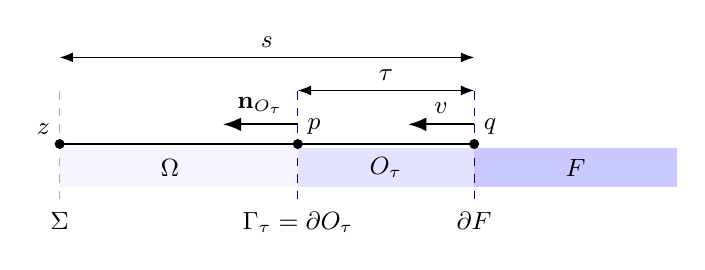
\begin{tikzpicture}[x=1.12cm,y=1cm,>=Latex,font=\small]
 \fill[blue!4] (0,-.55) rectangle (7,-.05);
 \fill[blue!11] (2.7,-.55) rectangle (7,-.05);
 \fill[blue!21] (4.7,-.55) rectangle (7,-.05);
 \draw[gray!65,dashed] (0,-.7)--(0,.7);
 \draw[blue!60!black,dashed] (2.7,-.7)--(2.7,.7);
 \draw[blue!60!black,dashed] (4.7,-.7)--(4.7,.7);
 \draw[thick] (0,0)--(4.7,0);
 \fill (0,0) circle (1.8pt);
 \fill (2.7,0) circle (1.8pt);
 \fill (4.7,0) circle (1.8pt);
 \node[above left] at (0,0) {$z$};
 \node[above right] at (2.7,0) {$p$};
 \node[above right] at (4.7,0) {$q$};
 \node[below] at (0,-.74) {$\Sigma$};
 \node[below] at (2.7,-.74) {$\Gamma_\tau=\partial O_\tau$};
 \node[below] at (4.7,-.74) {$\partial F$};
 \node at (1.25,-.3) {$\Omega$};
 \node at (3.7,-.3) {$O_\tau$};
 \node at (5.85,-.3) {$F$};
 \draw[<->] (0,1.1)--node[above] {$s$}(4.7,1.1);
 \draw[<->] (2.7,.68)--node[above] {$\tau$}(4.7,.68);
 \draw[->,thick] (2.7,.25)--(1.85,.25)
       node[midway,above] {$\mathbf n_{O_\tau}$};
 \draw[->,thick] (4.7,.25)--(3.95,.25)
       node[midway,above] {$v$};
\end{tikzpicture}
\caption{The offset construction along a minimizing segment in the
singleton-normal case. First take $F=\{\rho\ge s\}$, then enlarge it
by $\tau<s$ to $O_\tau$; the gap to $\Sigma$ on this segment is
$s-\tau$. The outward normals point toward $\Sigma$, hence equal
$-\nu$ in the exterior application. This local schematic asserts no
tubular coordinates at singular points.}
\label{fig:rpi:smoothing-offset}
\end{figure}

Let $C_R\ge0$ bound the negative part of the ambient Ricci curvature
on the fixed neighborhood. Along the touching geodesic, the normal
Riccati equation gives
\[
 H(\text{enlarged }D\text{ at }z)
        \le H(D\text{ at }p)+C_R(s-\tau).
\]
First-contact comparison with the accessible part of $\Sigma$ gives
$H(\text{enlarged }D\text{ at }z)\ge\gamma$.

Here is the endpoint argument if the enlargement is focal at $z$.
Localize $D$ near $p$ and shrink it strictly away from $p$, preserving
the touching segment, so that $p$ is the unique terminal footpoint.
In tangent coordinates with outward normal in the positive vertical
direction, replace its boundary graph $u$ by
$u-a|x|^2$, where $a>0$ can be arbitrarily small. This shrinks the
domain and increases its outward second fundamental form at contact
by $2a$ times the tangent metric. The boundary index form of the
original minimizing normal segment is nonnegative; the perturbation
adds $2a|J(0)|^2$ for each variation field $J$. Variations with
$J(0)=0$ have positive index because the segment is shorter than
the ambient conjugacy scale. Thus the perturbed segment is nonfocal
through its endpoint. Apply the Riccati comparison to the perturbed
domain and let $a\downarrow0$. Its mean curvature at contact tends
to that of $D$, proving also in this case that
\[
 H(D\text{ at }p)\ge\gamma-C_Rs.
\]

Suppose next that the normal cone contains a direction not parallel
to $v$. Convexity supplies a nontrivial one-sided angular arc through
$v$. Exponentiating this arc at radius $\tau$ produces a curve in
$\Gamma_\tau$. The test boundary has the same first derivative at
contact. Second-order comparison along the arc, even when it is
one-sided, therefore gives a principal curvature at least
$1/(2\tau)$ for small $\tau$. The exterior supporting ball gives
a lower bound $-C_F$ for all the other principal curvatures,
independent of $\tau$ for this fixed $F$. Hence
\[
 H(D\text{ at }p)\ge\frac1{2\tau}-(n-2)C_F.
\]
This exceeds any fixed lower bound when $\tau$ is sufficiently
small. The pointedness proved above excludes the remaining apparent
possibility of opposite normals without an angular arc.

Choose the regular value $s<\varepsilon$ sufficiently small that
$C_Rs<\varepsilon/4$. Then choose $\tau$ sufficiently small compared
with $s$, the reach of this fixed $F$, and its curvature constants.
The resulting $C^{1,1}$ hypersurface has outward mean curvature at
least $\gamma-\varepsilon/4$ in the barrier sense. At almost every
twice-differentiability point of a $C^{1,1}$ graph, quadratic test
functions give the same inequality for its classical almost-everywhere
mean curvature. The order of these choices is important: neither
the reach nor $C_F$ is asserted to remain uniform as $s\downarrow0$.

\paragraph{Smooth graph approximation.}
We use the following direct fact. A compact cooriented embedded
$C^{1,1}$ hypersurface with almost-everywhere outward mean curvature
at least $c$ has smooth embedded approximations converging in $C^1$
whose mean curvature is at least $c-o(1)$.

To prove it, choose a smooth ambient vector field $V$ uniformly
transverse to the hypersurface, by smoothly approximating its
continuous unit normal near the compact hypersurface. The $C^1$
inverse function theorem and compactness give a fixed flow tube for
$V$, in which each sufficiently short flow line meets the hypersurface
exactly once. Local graph convolution and a partition of unity give
a smooth $C^1$ approximation $\Gamma_0$ sufficiently close to lie in
this tube and remain uniformly transverse to $V$. Projection along
these fixed flow lines is a global diffeomorphism. The original
hypersurface is therefore the flow graph of a $C^{1,1}$ function
$u$ over $\Gamma_0$. This fixed transverse flow avoids any assumption
about the normal injectivity radius of an arbitrary $C^1$ approximation.

In local coordinates its mean-curvature operator has the form
\[
 H(u)=A^{ab}(x,u,Du)\,\partial_{ab}u+B(x,u,Du),
\]
where the coefficients are smooth on a compact set of allowed graph
jets. The sign of $A$ depends on the graph convention and is immaterial
for the following averaging argument. Choose a finite smooth atlas
with subordinate partition of unity $\chi_\alpha$ and smooth $u$
using normalized nonnegative convolution kernels
$\rho_{\alpha,\zeta}$. The functions $u_\zeta$ converge to $u$ in
$C^1$ and have uniformly bounded second derivatives. Their second
derivatives equal the partition-weighted averages of $D^2u$ plus
a uniformly vanishing term. Indeed, differentiating the partition
introduces differences $u_\zeta-u$ and $Du_\zeta-Du$, which tend
uniformly to zero, while the sums of the derivatives of the partition
vanish.

Because $D^2u$ is uniformly bounded, the coefficient replacement
inside those averages,
\[
 A(x,u_\zeta,Du_\zeta)\longmapsto A(y,u(y),Du(y)),
\]
gives a uniformly vanishing commutator. The
lower-order coefficients converge uniformly as well. Coordinate
changes and connection terms are included in $B$; their additional
smoothing errors are controlled by the same $C^1$ convergence.
Consequently
\[
 H(u_\zeta)(x)
 =\sum_\alpha\chi_\alpha(x)
    \int\rho_{\alpha,\zeta}(x,y)H(u)(y)\,dy+o(1)
 \ge c-o(1)
\]
uniformly in $x$, proving the asserted approximation.

Apply this construction to the fixed hypersurface $\Gamma_\tau$.
Its positive distance from $\Sigma$ ensures that a sufficiently
small $C^1$ perturbation remains inside $\Omega$. Choose the region
on the same side of the smoothed boundary that contains the deep
part of $\Omega$. It differs from $O_\tau$ only in a tubular
neighborhood of $\Gamma_\tau$. Choose the width of this neighborhood
smaller than both its distance from $\Sigma$ and
$\varepsilon-s$. The removed collar is then contained in the
$\varepsilon$-collar of $\Sigma$. Finally choose $\zeta$ so small
that the mean-curvature loss is less than $\varepsilon/2$. The
resulting region is $\Omega_\varepsilon$, and its mean curvature is
at least $\gamma-\varepsilon$. This proves the proposition.
\end{proof}

For the almost-minimizing frontiers used here, the accessible locus
is exactly the regular part. At a point touched by a ball contained
in the exterior, a tangent cone lies on one side of a plane. The
half-space property for minimizing boundaries and small-excess
regularity make the point regular. Conversely, a regular point has
a sufficiently small supporting ball on the chosen side. Thus the
smooth embeddedness and local one-sided hypotheses of
Proposition~\ref{prop:rpi:one-sided-smoothing} hold. The proposition
is applied to the full compact frontier. An application to only
selected boundary components would also require a positive distance
from the remaining components; compactness of their union alone
does not imply that separation.

\paragraph{Application to a detached frontier.}
Let $E'$ be a detached minimizing exterior from the signed
variational construction, with $H_\nu\le-\gamma$ on its regular
frontier. Apply the proposition to $\Omega=E'$.
Its outward normal at the inner frontier is $-\nu$, so
$H_{\mathrm{out},\Omega}=-H_\nu\ge\gamma$. With
$\varepsilon=j^{-1}$, write $\Omega_j=\Omega_{j^{-1}}$. Since
$\Omega_j\subset\Omega$, the new frontier lies toward the
asymptotically flat end. With the end-oriented normal it satisfies
\begin{equation}\label{eq:rpi:smoothing-sign}
 H_\nu(\partial\Omega_j)\le-\gamma+j^{-1}<0
\end{equation}
for large $j$. Its compact removed region contains the original
removed region. In the variational definition of capacity this makes
the admissible class smaller, and hence
\begin{equation}\label{eq:rpi:capacity-monotonicity}
 \mathfrak c(\partial\Omega_j,h)\ge\mathfrak c(\Sigma,h).
\end{equation}
If $\Omega_j$ has bounded components, retain only the component
containing the asymptotic end. This selects whole components of its
smooth compact boundary, preserves the curvature sign, and enlarges
the conductor further. The same capacity comparison therefore holds
for the resulting connected smooth exterior. The argument uses only
the shrinking collar, the curvature sign and conductor inclusion;
no boundary-area convergence is needed.

This smooth exterior is complete with its boundary included. For
each fixed $\varepsilon$, the harmonic perturbation is uniformly
comparable with the starting metric, and the retained closed
exterior lies a positive distance from the original frontier.
The finite-length concatenation argument in
Lemma~\ref{lem:g-detachment} therefore gives completeness for its
intrinsic length distance. These are the smooth boundary and
completeness properties needed in the mass--capacity lemma below.

\section{Positive mass and the mass--capacity inequality}
\label{sec:rpi:smooth-repair}

The preceding construction reduces the singular-frontier argument
to a smooth mass--capacity inequality. We prove that inequality
from a positive mass theorem, independently of
Theorem~\ref{thm:rpi}. The conformal-flow argument at this stage
has a harmonically flat end, and that is the class we need. A harmonically flat
end has metric $U^{4/(n-2)}\delta$, with $U>0$ Euclidean harmonic and
$U\to1$. We use the independently stated smooth positive mass result
\cite[Corollary~1.6]{BrendleWang2026}. Its actual hypotheses are strict
positive scalar curvature and an all-order end expansion
\begin{equation}\label{eq:rpi:bw-end}
 g=(1+\alpha r^{2-n})\delta+O_j(r^{2-n-\sigma}),\qquad \sigma>0,
\end{equation}
for every fixed $j$. The complete smooth manifold in that corollary
and its governing definitions has no orientability assumption. In
dimensions at least four other ends are permitted. Its mass is
$(n-1)\alpha$, whereas our ADM mass is
$(n-2)\alpha/2$; their signs agree. The following argument uses it only
for $n\ge8$; the lower-dimensional numerical positive mass theorem
and \cite{BrayLee2009} provide the classical alternative.

The dimension-descent proof of the cited theorem uses a singular-set
covering estimate for weighted perimeter minimizers with a volume
forcing. Appendix~\ref{sec:rpi:weighted-minimizers} proves the
needed estimate for that class, using
\cite[Theorem~1.3]{NaberValtorta2020}; its role in
\cite[Definition~3.19, Lemma~3.20, and Theorem~3.34]{BrendleWang2026}
is specified there. With that input accounted for, the remaining
steps of the mass--capacity proof concern smooth metrics: first
pass from strict to nonnegative scalar curvature on harmonic ends,
then double the smooth exterior and repair its seam.

\subsection{Nonnegative mass on harmonic ends}

\begin{lemma}\label{lem:rpi:harmonic-pmt}
A smooth complete boundaryless manifold of dimension $n\ge8$ with finitely many
ends, all harmonically flat, and nonnegative scalar curvature has nonnegative
ADM mass at each end.
\end{lemma}
\begin{proof}
Work on the connected component containing the chosen end.
Choose a positive smooth function $\rho$, equal to $r^{-n-\beta}$ on
each distant end, with $0<\beta<1$. The global Sobolev inequality on a
manifold with finitely many Euclidean ends, followed by exhaustion,
gives the positive solution of
\[
 -\Delta v=\rho,\qquad v\longrightarrow0\quad\hbox{on every end}.
\]
More explicitly, $\rho\in L^{2n/(n+2)}$, so the energy completion of
compactly supported functions gives a weak solution by the coercive
Dirichlet form. Positivity follows by testing the negative part.
The local elliptic estimates and end barriers give a bounded smooth
solution; the homogeneous decaying maximum principle gives uniqueness.
On each harmonically flat end, $Uv$ satisfies a Euclidean Poisson
equation with right side $-U^{(n+2)/(n-2)}\rho$. The Newton potential,
split into inner, comparable, and outer annuli, gives
\[
 v=A r^{2-n}+O_j(r^{2-n-\beta'})
 \quad\text{for }0<\beta'<\beta.
\]
Equivalently, subtract the Newton kernel's monopole and use the
finite $\beta'$ moment of the right-hand side. The contribution of
the finite inner boundary is a decaying harmonic function with the
same type of expansion. Scaled interior estimates give all fixed
orders of derivatives. Thus $(1+t v)^{4/(n-2)}g$ satisfies
Equation~\eqref{eq:rpi:bw-end}, is complete, and has strictly positive
scalar curvature for every $t>0$, since
\[
 -\frac{4(n-1)}{n-2}\Delta(1+t v)+R_g(1+t v)>0.
\]
Apply the cited positive mass theorem and let $t\downarrow0$.
The ADM mass changes by $2tA$ at the chosen end, which proves the
claim.
\end{proof}

\subsection{Doubling and conformal repair}

We can now turn the capacity of a smooth boundary into a mass
decrease on a complete manifold. The doubling must keep its second
end complete while positive mass is applied; a positive parameter
will do this, and it can be sent to zero afterward.

The following doubling, seam smoothing, and conformal repair have
their three-dimensional antecedent in
\cite[Definition~17 and Theorem~9, pp.~206--211]{Bray2001}.
The normalization there gives the same three-dimensional capacity
bound. The higher-dimensional positive-mass input is instead the
smooth theorem and the reduction just established.

\begin{lemma}[Smooth mass--capacity inequality]
\label{lem:rpi:mass-capacity}
Let $(N,h)$, of dimension $n\ge8$, be a smooth connected exterior,
complete including its compact smooth boundary, with exactly one end
and compact end complement. Suppose the end is harmonically flat
and the scalar curvature is nonnegative. Write $\Gamma$ for its
boundary. If $H_\nu\le0$ for the normal toward the end, then
$m_{\rm ADM}(h)\ge\mathfrak c(\Gamma,h)$.
\end{lemma}
\begin{proof}
If $\Gamma$ is empty, its capacity is zero and the assertion is
Lemma~\ref{lem:rpi:harmonic-pmt}. Assume henceforth that $\Gamma$
is nonempty. Let $\phi=1-w$, where $w$ is the potential in
Equation~\eqref{eq:rpi:capacity}, and write $c=\mathfrak c(\Gamma,h)$.
On the doubled manifold define $\psi=\phi$ on the first copy and
$\psi=-\phi$ on the second. In signed normal distance across the seam,
$\psi$ and its first derivative agree: its value is zero and both
normal derivatives equal $\partial_\nu\phi$. For $0<a<1$, put
\[
 V_a=\frac{1+a+(1-a)\psi}{2},\qquad
 h_a=V_a^{4/(n-2)}\bar h,
\]
where $\bar h$ is the doubled corner metric. The factor is bounded
below by $a$, tends to one at the first end and to $a$ at the second,
and is weakly harmonic. Consequently $h_a$ is complete, has two
harmonically flat ends after constant rescaling at the second, and has
nonnegative scalar curvature away from the seam.

Choose the common transverse normal from the second copy to the first.
The two mean curvatures of $\bar h$ with this normal are $-H_\nu$ and
$H_\nu$. Their jump in the corner condition is therefore $-2H_\nu\ge0$.
The normal derivative of $V_a$ is continuous, so its contribution
cancels in the conformal jump formula; the jump for $h_a$ has the same
sign. We now explain the analytic smoothing step to avoid extending
the dimensional or topological statement of a corner theorem without
justification.

Apply the local Gaussian-collar construction of
\cite[Section~3, Proposition~3.1 and Equation~(36)]{Miao2002}.
Its tensor convolution uses the coorientation of this collar and
is independent of the topology or number of ends outside it.
It gives uniformly comparable $C^2$ metrics, equal to $h_a$ off
a shrinking collar, whose negative scalar curvature has a uniform
bound. For each fixed collar parameter, approximate this metric
in $C^2$ by a smooth metric, keeping it unchanged outside a slightly
larger collar. Scalar curvature is continuous in the metric's
$C^2$ jets, so choosing the approximation sufficiently close
preserves the negative-scalar bound up to a fixed enlargement.
Denote these smooth metrics by $h_{a,\delta}$.
Their negative scalar curvature is supported in a collar whose
volume tends to zero. Choose a smooth
$q_\delta\ge(R_{h_{a,\delta}})_-$, uniformly bounded and supported in
a slightly larger shrinking collar. Solve
\[
 \Delta_{h_{a,\delta}} z_\delta+
       \frac{n-2}{4(n-1)}q_\delta z_\delta=0,
 \qquad z_\delta\longrightarrow1\quad\text{at both ends}.
\]
Here is the required existence and mass estimate on this two-ended
manifold. Put $a_n=4(n-1)/(n-2)$, $2^*=2n/(n-2)$ and
$p=2n/(n+2)$. A fixed complete metric with these ends satisfies
$\|f\|_{2^*}^2\le S_a\int|df|^2$: combine the Euclidean end
inequalities with a compact-core Poincar\'e estimate having trace on
one fixed end annulus. Uniform metric comparison gives the same
inequality for $h_{a,\delta}$, uniformly in small $\delta$.
Since $\|q_\delta\|_{n/2}\to0$, the form
\[
 B_\delta(f,f)=a_n\int|df|^2-\int q_\delta f^2
       \ge\frac{a_n}{2}\int|df|^2
\]
is coercive on the homogeneous energy completion of compactly
supported smooth functions. Solving
$B_\delta(u_\delta,f)=\int q_\delta f$ gives
\[
 \|u_\delta\|_{2^*}+\|du_\delta\|_2
       \le C_a\|q_\delta\|_p.
\]
Testing the negative part gives $u_\delta\ge0$. Local elliptic
regularity and the harmonic exterior equation give a smooth solution
$z_\delta=1+u_\delta\ge1$, tending to one on both ends; the end
limits also follow from $u_\delta\in L^{2^*}$.
The corrected smooth metric
$z_\delta^{4/(n-2)}h_{a,\delta}$ has nonnegative scalar curvature.
It is still harmonically flat at both ends. In separately normalized
end coordinates write
$u_\delta=A_{i,\delta}r_i^{2-n}+O_j(r_i^{1-n})$;
the coefficients are nonnegative because $u_\delta\ge0$.
Flux integration over both ends gives
\[
 a_n(n-2)\omega\sum_{i=1}^2A_{i,\delta}
   =\int q_\delta z_\delta\,dV
   \le\|q_\delta\|_1+C_a\|q_\delta\|_p^2=o(1).
\]
Thus each coefficient tends to zero, and each end mass converges to
that of $h_a$.
Lemma~\ref{lem:rpi:harmonic-pmt} proves nonnegativity of this limiting
mass. This argument is local at the seam and accommodates both ends;
it does not invoke the one-ended global statement of
\cite[Theorem~1]{Miao2002} outside its stated class.

On the retained end,
\[
 \phi=1-cr^{2-n}+O_j(r^{1-n}),\qquad
 V_a=1-\tfrac12(1-a)cr^{2-n}+O_j(r^{1-n}),
\]
so the conformal ADM formula gives
\[
 0\le m_{\rm ADM}(h_a)=m_{\rm ADM}(h)-(1-a)c.
\]
Let $a\downarrow0$. Both ends remained complete for every application
of the smooth positive mass theorem; no theorem about a compactified
point was used.
\end{proof}

The signed variational construction, one-sided smoothing and
Lemma~\ref{lem:rpi:mass-capacity} now give the smooth comparison
needed for a singular time slice: an enclosing smooth conductor has
at least the original capacity, while its end mass is unchanged by
moving the frontier. Section~\ref{sec:rpi:flow-mass-capacity} applies
this comparison to a small harmonic perturbation and removes that
perturbation. The same positive two-ended construction will provide
the complete inputs used in Section~\ref{sec:rpi:lee-completion}.

\section{Mass and capacity along the flow}
\label{sec:rpi:flow-mass-capacity}

The smooth comparison applies to every flow slice after a small
harmonic perturbation. Together with the end expansion, it gives the
mass decrease that drives the remaining argument.

\begin{proposition}[Mass and capacity of the conformal flow]
\label{prop:rpi:mass-evolution}
For the conformal flow of Lemma~\ref{lem:rpi:flow-construction} in
dimension $n\ge8$, with nonempty initial frontier and harmonically flat
initial end, let $m(t)$
be its ADM mass in normalized coordinates and let
$c_t=\mathfrak c(\Sigma_t,g_t)$. Then
\[
 m(t)\ge c_t\ge0,\qquad \mu(t):=m(t)-c_t\ge0.
\]
The mass is locally absolutely continuous and satisfies
$m'(t)=-2\mu(t)$ almost everywhere.
\end{proposition}

\begin{proof}
Fix a slice with normalized metric $h$, and write $m,c,w$ for its mass, capacity, and capacitary
potential in normalized end coordinates. For $\lambda>0$ small set
$p=1+\lambda w$ and $h_\lambda=p^{4/d}h$.
Conformal harmonicity and the end expansions give
\[
 w_{\Sigma,\lambda}=\frac{(1+\lambda)w}{p},\qquad
 c_{\Sigma,\lambda}=(1+\lambda)c,\qquad
 m_\lambda=m+2\lambda c.
\]
This is the earlier separating perturbation with
$\lambda=\varepsilon/(1-\varepsilon)$. Its detached smooth enclosure
$\Gamma$ has $H_\nu<0$. Capacity monotonicity and
Lemma~\ref{lem:rpi:mass-capacity}, applied to its smooth exterior, give
\[
 m+2\lambda c=m_\lambda\ge c_\Gamma
       \ge (1+\lambda)c.
\]
Sending $\lambda\downarrow0$ proves $m\ge c$ on the original time
slice.

For the evolution formula, write the initial end as
$g_0=H^{4/d}\delta$, where $H>0$,
$\Delta_\delta H=0$, and $H\to1$. The products $Hu_t$ and $Hv_t$
are Euclidean harmonic on the end. Expanding them there and dividing
by $H$ gives, for any fixed $0<\beta<1$,
\[
 u_t=e^{-t}+B(t)r^{-d}+O_1(r^{-d-\beta}),\qquad
 v_t=-e^{-t}+b(t)r^{-d}+O_1(r^{-d-\beta}),\qquad B'=b,
 \quad B(0)=0.
\]
Flux identification and normalization of the end coordinates give
\[
 c_t=e^{-t}(B+b),\qquad
 m(t)=e^{-2t}m(0)+2e^{-t}B(t),\qquad
 \mu(t)=m(t)-c_t.
\]
Since $B$ is locally absolutely continuous, so is $m$, and
differentiation gives $m'=-2\mu$ almost everywhere.
\end{proof}

A restarted flow at
time $s$ has conformal and evolution factors $u_{s+t}/u_s$ and
$v_{s+t}/u_s$. The denominator stays fixed at the restart time.
The capacitary potential has finite homogeneous energy in every
dimension; its unweighted $L^2$ tail is also finite when $n\ge5$,
since it is controlled by $\int_R^\infty r^{3-n}\,dr$.

\paragraph{The normalized end factors.}
Let $\Phi_t(x)=e^{2t/d}x$ map the
normalized coordinate $x$ to the original coordinate. The normalized
flow metric is $G_t=\Phi_t^*g_t$ on this end. Transport the flow and
velocity factors by
\[
 U_t=e^tu_t\circ\Phi_t,\qquad V_t=e^tv_t\circ\Phi_t.
\]
The normalized background metric and its factor are
\[
 h_t=H\circ\Phi_t,\qquad
 \bar G_t=e^{-4t/d}\Phi_t^*g_0=h_t^{4/d}\delta.
\]
The velocity $V_t$ is $\bar G_t$-harmonic on the portion of the
normalized exterior in this end chart.
Define the total factors and the auxiliary relative factor as follows:
\[
\begin{array}{c|c|c}
 \text{role}&\text{relative factor}&\text{Euclidean-harmonic factor}\\ \hline
 \text{flow metric}&U_t&F_t=h_tU_t\\
 \text{velocity}&V_t&Z_t=h_tV_t\\
 \text{auxiliary metric}&W_t=(U_t-V_t)/2&J_t=h_tW_t
\end{array}
\]
Then $G_t=F_t^{4/d}\delta$, and
\[
 J_t=\frac{F_t-Z_t}{2}
     =F_t\bigl(1-(w_t\circ\Phi_t)/2\bigr),\qquad
 \widetilde G_t=J_t^{4/d}\delta.
\]
The total factors are harmonic outside a sphere enclosing the current
frontier and compact core. Their constant terms are $1,-1,1$,
respectively; the masses of the flow and auxiliary metrics are $m(t)$
and $\mu(t)$.
Section~\ref{sec:rpi:lee-completion} constructs complete smooth
metrics whose end factors approximate $J_t$, allowing a quantitative
positive-mass estimate to control it.

The flow calculation is first made for harmonically flat ends.
Section~\ref{sec:rpi:density-repair} then proves the passage to the
general asymptotically flat metrics used here. It first introduces a
strict smooth boundary, proves a Dirichlet conformal approximation
with mass convergence, and takes a detached minimizing enclosure.
The resulting metric comparison controls all enclosing areas.

\section{Mass decay and the enclosure radius}
\label{sec:rpi:flow-estimates}

Area preservation and Proposition~\ref{prop:rpi:mass-evolution} reduce
the argument to the decay of $\mu(t)=m(t)-c_t$ and the location of the
frontier. The next estimates provide a fixed harmonic tail in normalized
coordinates, on which the quantitative positive-mass theorem will apply.
Put $d=n-2$ and $q=2(n-1)/d$, and retain
$\omega=|S^{n-1}|$ for the Euclidean area of the unit sphere.

\begin{proposition}[Vanishing deficit and bounded normalized radius]
\label{prop:rpi:flow-estimates}
For the flow in Proposition~\ref{prop:rpi:mass-evolution},
$\mu(t)\to0$ as $t\to\infty$. There is a fixed $R_{\max}$ such that
\begin{equation}\label{eq:rpi:radius-bound}
 \Sigma_t\subset B_{R_{\max}e^{2t/d}}\qquad(t\ge0).
\end{equation}
Here the radius is measured in the original end coordinates, with the
compact core included in the ball. Equivalently, every normalized
frontier lies in $B_{R_{\max}}$.
\end{proposition}

\begin{proof}
\textbf{The integrated mass identity.}\quad
Since $B'=b$ and $B(0)=0$,
\[
 \frac{d}{dt}(e^{-t}B(t))=e^{-t}(b(t)-B(t)).
\]
Consequently
\[
 \int_0^t\mu(s)\,ds
 =\frac12(1-e^{-2t})m(0)-e^{-t}B(t)
 =\frac{m(0)-m(t)}2.
\]
This supplies integrability of the nonnegative
$\mu$. Set $a=m-2\mu=2c_t-m$.
Nesting and the maximum principle make $e^tv_t$ nondecreasing:
the later potential is zero on the larger filled set and both have
limit $-1$ at infinity. Its end coefficient $e^tb(t)$ is therefore
nondecreasing. Since
\[
 e^{2t}a(t)=2e^tb(t)-m(0),
\]
the same holds for $e^{2t}a(t)$. This implies, distributionally,
$Da+2a\,dt\geq0$. Substitution of the integral identity gives
monotonicity of $3m-2\mu+2\int_0^t m$ (up to a constant).
Thus for $h>0$,
\[
 \mu(t+h)-\mu(t)
 \leq\frac32\bigl(m(t+h)-m(t)\bigr)
       +\int_t^{t+h}m(s)\,ds
 \leq h m(0).
\]
This one-sided slope bound and integrability imply
$\mu(t)\to0$: a value at least $\varepsilon>0$ forces an
interval immediately before it on which the integral is bounded below
by a positive constant depending only on $\varepsilon,m(0)$.
If $m(0)=0$, nonnegativity and mass monotonicity give $m=0$;
the same slope bound excludes positive point values of $\mu$.

\paragraph{The escaping-point ball.}
Let $a=e^{2/d}$ and $R(s)=R_{\max}e^{2s/d}$. Suppose
that containment holds for $0\le s\le T$ but there is a point
$p\in\Sigma_{T+1}$ with $|p|\geq aR(T)$. Use the ball
\[
 \rho=\frac{a-1}{2}R(T),\qquad
 \overline{B_\rho(p)}\subset\{|y|>R(T)\}.
\]
Here the balls are Euclidean balls in the original end coordinates.
Choose $R_{\max}$ so the indicated exterior avoids the initial obstacle
and $\tfrac12\delta\leq g_0\leq2\delta$ there.

To estimate the metric on this ball, use its total harmonic conformal factor.
Write $g_0=H^{4/d}\delta$ on the initial end, where $\Delta_\delta H=0$
and $H\to1$. Then $Hv_s$ is Euclidean harmonic outside $\Sigma_s$.
If $\Sigma_s\subset B_{R(s)}$, its boundary value on $S_{R(s)}$
is nonpositive and its limit at infinity is $-e^{-s}$, so
\[
 Hv_s(y)\leq e^{-s}\left[\left(\frac{R(s)}{|y|}\right)^d-1\right]
 \qquad (|y|\geq R(s)).
\]
Using $v_s\leq0$ on the remaining time interval gives, for $r=|y|\geq R(T)$,
\[
 H u_{T+1}\leq H-1+e^{-T}+(e^T-1)R_{\max}^d r^{-d}.
\]
Choose $H-1\leq C_0r^{-d}$ and $R_{\max}^d\geq C_0$.
The last expression is at most $2e^{-T}$. Taking also $H\geq1/2$
gives the concrete bounds
\[
 e^{-T-1}\leq u_{T+1}\leq K e^{-T},\qquad K=4,
 \qquad r\geq R(T).
\]

Every finite-perimeter variation supported in $B_\rho(p)$ remains an
admissible enclosure. Comparison of area elements therefore makes
$\Sigma_{T+1}$ Euclidean perimeter-quasiminimizing there, with ratio
\[
 \gamma=2^{n-1}(eK)^q.
\]
The isoperimetric proof of the density estimate, using the competitors
that fill or delete a ball, applies at every measure-theoretic boundary
point, including a singular point. It yields
\[
 \mathcal H_\delta^{n-1}(\Sigma_{T+1}\cap B_\rho(p))
 \geq c(n,\gamma)\rho^{n-1}.
\]
It follows that the fixed area satisfies
\[
 \begin{split}
 A&\geq 2^{-(n-1)/2}e^{-q(T+1)}
       c(n,\gamma)\rho^{n-1}\\
  &=2^{-(n-1)/2}c(n,\gamma)e^{-q}
       \left(\frac{e^{2/d}-1}{2}\right)^{n-1}R_{\max}^{n-1}.
 \end{split}
\]
All time factors cancel. The constants are independent of $T$ and of
further enlargement of $R_{\max}$, giving the required contradiction.
To cover all times, enlarge $R_{\max}$ to obtain containment on $[0,1]$
from the finite-time support bound. If containment holds on
$[0,N]$, apply the argument at each $t\in[N,N+1]$ with $T=t-1$.
This proves Equation~\eqref{eq:rpi:radius-bound} at every real time.
\end{proof}

\section{Complete metrics and the auxiliary end factor}
\label{sec:rpi:lee-completion}

Lee's quantitative positive-mass estimate turns small mass into control
of a harmonic end factor. To apply it to $J_t$, we construct complete
smooth metrics whose masses tend to zero and whose end factors approach
$J_t$. The construction keeps a fixed coordinate tail while allowing
the compact interior to vary. Throughout, $n\ge8$ and $d=n-2$.

\begin{proposition}[Complete approximants and the auxiliary factor]
\label{prop:rpi:complete-end-factors}
For the normalized flow of Proposition~\ref{prop:rpi:mass-evolution}
there are fixed radii $R_c<R_1$
and complete smooth connected boundaryless one-ended metrics with nonnegative scalar
curvature, harmonic end factors $\mathcal Z_t$ on $\{r>R_1\}$,
and masses $\mathcal M_t$, such that
\[
 0\le\mathcal M_t\longrightarrow0,\qquad
 \sup_{r\ge2R_1}r^d|\mathcal Z_t-J_t|\longrightarrow0.
\]
The radius $R_c$ encloses every normalized frontier and compact core.
For every fixed $s>R_c$,
\begin{equation}\label{eq:rpi:auxiliary-weighted-limit}
 \sup_{r\ge s}r^d|J_t-1|\longrightarrow0.
\end{equation}
\end{proposition}

We first isolate the quantitative input, so that the construction can
be read separately from the verification of its positive-mass hypotheses.

\begin{lemma}[Quantitative positive mass on one harmonic end]
\label{lem:rpi:quantitative-one-end}
For each $n\ge8$ there is a fixed constant $\ell_n>1$ such that,
for every $\eta>0$, there is $\delta(n,\eta)>0$ with the following
property. Let $(N,h)$ be a smooth complete connected boundaryless
$n$-manifold with $R_h\ge0$. Suppose that outside a compact set it
consists of a single coordinate end $\{r>R\}$, where $R>0$, and that
on this end
\[
 h=Z^{4/(n-2)}\delta,\qquad Z>0,\qquad
 \Delta_\delta Z=0,\qquad Z\longrightarrow1.
\]
Writing $d=n-2$ and $m=m_{\rm ADM}(h)$, we have
\[
 m<\delta(n,\eta)R^d
 \quad\Longrightarrow\quad
 \sup_{r>\ell_nR}|Z-1|<\eta.
\]
\end{lemma}

\begin{proof}
Rescale the metric by $R^{-2}$ and the coordinates by $R^{-1}$.
The harmonic coordinate radius becomes one, and the mass becomes
$m/R^d$. We apply the argument of
\cite[Theorem~1.3]{Lee2007NearEquality} at this scale. Its formal
hypothesis concerns every complete asymptotically flat metric on the
underlying manifold; we verify that the positive-mass statements used
in its proof follow here from Lemma~\ref{lem:rpi:harmonic-pmt}.
The one-end assumption also identifies the mass flux in Lee's
Lemma~2.1 with the flux in the divergence integral over the entire
manifold.

The scalar-flat reduction of
\cite[Lemma~2.5]{Lee2007NearEquality} gives a metric
$k=f^{4/d}h$ with $f>0$ and $f\to1$. The factor is bounded above
and below by positive constants, so $k$ remains smooth and complete.
Its end factor $Zf$ is Euclidean harmonic. For this scalar-flat
reference metric, Lee uses the variations
\[
 k_s=k+s\zeta\operatorname{Ric}(k),\qquad
 \widehat k_s=u_s^{4/d}k_s,
\]
where the cutoff $\zeta$ is compactly supported and
$\widehat k_s$ is scalar-flat. Outside the support of $\zeta$, the
product of the old end factor and $u_s$ is Euclidean harmonic.
The conformal scalar-curvature identity gives
\[
 c_n=\frac{n-2}{4(n-1)},\qquad
 L_s=\Delta_{k_s}-c_nR_{k_s},\qquad
 L_s(u_s-1)=c_nR_{k_s}.
\]
Both scalar-curvature coefficients in the operator definition and
inhomogeneous equation preceding Lee's Lemma~2.4 must have this value,
as in the earlier conformal equation in that paper. Lemma~2.4 estimates
$\Delta_k$, and the ensuing perturbation argument applies with the
corrected fixed dimensional coefficient. Its exterior estimates give
$u_s-1=O(|s|)$ uniformly. On the compact region away from the
perturbation, $u_s-1$ is harmonic, so the maximum principle extends
this bound throughout the manifold. For sufficiently small $|s|$,
$1/2\le u_s\le3/2$. The perturbed and conformally corrected metrics
are therefore smooth and complete.

The scalar-flat argument uses nonnegativity of the varied mass at a
small negative parameter
\cite[proof following Lemma~2.2]{Lee2007NearEquality}. This follows
from Lemma~\ref{lem:rpi:harmonic-pmt}, since every varied metric has
a harmonic end outside a compact set. The same lemma gives
$m_{\rm ADM}(k)\ge0$ after the initial scalar-flat reduction.
Lee's Lemma~2.5 gives $m_{\rm ADM}(k)\le m_{\rm ADM}(h)$ and
controls the end-factor difference by the mass difference.
Thus all the required
positive-mass inputs hold, without a spin or orientability assumption.
The constants in Lee's estimates depend only on dimension and the
target error at the normalized radius, not on the compact interior.
Restoring the scale $R$ gives the asserted implication.
\end{proof}

\begin{proof}[Proof of Proposition~\ref{prop:rpi:complete-end-factors}]
We use the following elementary harmonic estimate.  If $q\ge0$ is
Euclidean harmonic on $\{r>R\}$, tends to zero, and has expansion
$q=b r^{-d}+O(r^{-d-1})$, then
\begin{equation}\label{eq:rpi:positive-harmonic-monopole}
 0\le q(x)\le C(n)b r^{-d}\qquad(r\ge2R).
\end{equation}
Indeed, its spherical average is exactly $b r^{-d}$, and the Harnack
inequality on scaled annuli bounds its maximum on a sphere by a
dimensional constant times this average.  In particular, the constant
does not depend on the geometry inside $B_R$.

\paragraph{A smooth reduction from two ends to one.}
Let $(N,k)$ be a smooth complete connected boundaryless manifold with
exactly two harmonically flat ends and compact end complement, and
suppose $R_k\ge0$. Designate one end for retention. There is a
harmonic function $\chi$ tending to one on that end and zero on the
other, with $0<\chi<1$.  To construct it, choose a smooth function
constant with these values outside a compact set and minimize its
Dirichlet energy after addition of the homogeneous energy space.
The global Sobolev inequality gives the solution; truncation and the
strong maximum principle give its bounds.  Exterior elliptic estimates
give the stated end limits and expansions.

Write $k=Z_i^{4/d}\delta$ on either end.  Then $Z_i\chi$ is Euclidean
harmonic.  On the end to be filled,
\[
 Z_2\chi=b_2r^{-d}+O_j(r^{-d-1}),\qquad b_2>0.
\]
Positivity of $b_2$ follows by comparison with a positive multiple of
$r^{-d}$ from any fixed coordinate sphere.  Under inversion
$x=y/|y|^2$, the factor
\[
 |y|^{-d}(Z_2\chi)(y/|y|^2)
\]
extends harmonically across $y=0$ with value $b_2$.  Thus
$\chi^{4/d}k$ extends to a smooth metric after adding one point.
The filled manifold is complete, has one end, and has nonnegative
scalar curvature, since
$R_{\chi^{4/d}k}=\chi^{-4/d}R_k$ away from the added point and is zero
near that point.

At the retained end write
$\chi=1-A r^{-d}+O_j(r^{-d-1})$.  If $M=m_{\rm ADM}(k)$, the filled
metric has mass $M-2A$.  The function $Z_1(1-\chi)$ is nonnegative
Euclidean harmonic with monopole $A$.  Consequently
\begin{equation}\label{eq:rpi:one-end-reduction}
 0\le M-2A\le M,\qquad
 |Z_1-Z_1\chi|\le C(n)M r^{-d}\quad(r\ge2R),
\end{equation}
where the first inequality uses
Lemma~\ref{lem:rpi:harmonic-pmt} on the smooth filled manifold.
The estimate depends only on the retained-end coordinate radius and
mass; the second end may vary with the compact interior.

\paragraph{A common coordinate tail.}
Use the normalized metric $G_t$ and total harmonic factor $F_t$
from Section~\ref{sec:rpi:flow-mass-capacity}. In this subsection,
$\Sigma_t,w_t$ denote its frontier and capacitary potential in these
coordinates; the latter is the pullback previously written
$w_t\circ\Phi_t$. A coordinate ball includes the compact core when
the whole exterior is under discussion. The mass, capacity, and deficit
remain $m(t)$, $c_t$, and $\mu(t)=m(t)-c_t$.
The preceding radius bound and harmonic estimates give
$\Sigma_t\subset B_{R_c}$, the factors $F_t$ are uniformly bounded on
a fixed sphere outside $B_{R_c}$, and
\[
 0\le c_t\le m(t)\le m(0),\qquad \mu(t)\longrightarrow0.
\]
Indeed, take $T=t-1$ in the radius estimate: $U_t\le4e$ on the
normalized tail $r\ge R_{\max}$ for $t\ge1$. The initial bounded time
interval is covered by the finite-time flow bounds. Multiplication by
the uniformly bounded initial harmonic factor gives the asserted
bound for $F_t$. Increasing $R_c$ once includes that sphere. Let $w_t$ be the
capacitary potential equal to one at $\Sigma_t$ and zero at infinity.

For $0<\lambda<1$ put $p=1+\lambda w_t$ and
$h_{t,\lambda}=p^{4/d}G_t$.  The detachment and smoothing construction
above provides a smooth enclosing boundary $\Gamma$ with
$H_\nu^\Gamma<0$.  It can be chosen in a ball $B_{R_1}$ whose radius
is independent of $t$ and $\lambda$.  Here is the confinement
argument.  On the common coordinate end the positive harmonic factor
$F_tp$ has a uniform bound on $S_{R_c}$ and tends to one.  The maximum
principle and scaled gradient estimates give
\[
 |F_tp-1|+r|D(F_tp)|\le C(R_c/r)^d\quad(r\ge2R_c).
\]
Thus all coordinate spheres beyond a fixed $R_*$ have positive
outward mean curvature in $h_{t,\lambda}$. Write $K_t$ for the
original conductor and $L$ for its detached minimizing enlargement.
The functional minimized by $L$ is
\[
 \mathcal F(L)=P_{h_{t,\lambda}}(L)+
       \theta\int_{L\setminus K_t}h_0\,dV_{h_{t,\lambda}},
 \qquad h_0\ge0 .
\]
Let $X$ be the outward unit normal to the coordinate spheres.
For almost every $s>R_*$, the finite-perimeter divergence formula
on $L\cap\{r>s\}$ gives
\[
 P(L\cap\{r<s\})
 \le P(L)-\int_{L\cap\{r>s\}}\operatorname{div}X\,dV.
\]
Both the perimeter and the nonnegative volume penalty decrease under
clipping, strictly if the removed tail has positive volume.  Minimality
therefore confines $L$ to $B_{R_*}$.  The subsequent smooth boundaries
lie in shrinking collars, so they lie in $B_{R_1}$ for one
fixed $R_1>R_*$.  Fix such a smoothing index before doubling.
Thus the coordinate tail is fixed even when the separation distance
and smoothing parameters vary.

\paragraph{The capacity comparison and the completed end.}
Suppress $t$ temporarily and put $h=G_t$, $F=F_t$, $w=w_t$, $c=c_t$,
$m=m(t)$, $\mu=\mu(t)$.  The potential and capacity of the original
conductor for $h_\lambda=p^{4/d}h$ are exactly
\begin{equation}\label{eq:rpi:perturbed-capacity-exact}
 w_{\Sigma,\lambda}=\frac{(1+\lambda)w}{p},\qquad
 c_{\Sigma,\lambda}=(1+\lambda)c,\qquad
 m_\lambda=m+2\lambda c.
\end{equation}
These identities follow from the harmonic conformal transformation
formula and the end expansions.  If $w_\Gamma$ is the potential of
$\Gamma$ for $h_\lambda$ and $c_\Gamma$ its capacity, enclosure
monotonicity and Lemma~\ref{lem:rpi:mass-capacity} give
\[
 0\le D_\Gamma:=c_\Gamma-c_{\Sigma,\lambda}
 \le m_\lambda-c_{\Sigma,\lambda}=\mu+\lambda c.
\]
On the common tail the function
$Fp(w_\Gamma-w_{\Sigma,\lambda})$ is nonnegative Euclidean harmonic
with monopole $D_\Gamma$.  Its sign follows from the maximum
principle on the exterior of $\Gamma$.

For $0<a<1$ the positive two-ended doubling construction in
Lemma~\ref{lem:rpi:mass-capacity} has retained end factor
\[
 B=Fp\left(1-\frac{1-a}{2}w_\Gamma\right)
\]
and retained end mass
\[
 m_B=m_\lambda-(1-a)c_\Gamma
 \le \mu+\lambda c+a m_\lambda .
\]
The Miao smoothing and its conformal correction produce smooth
complete two-ended metrics with $R\ge0$ and retained factor $Bz_\delta$
on $\{r>R_1\}$.  In the notation of that proof,
$z_\delta\ge1$, and
\[
 e_\delta:=B(z_\delta-1)\ge0
\]
is Euclidean harmonic on the common tail with monopole
$A_\delta\to0$.  Their retained masses are
$M_\delta=m_B+2A_\delta\ge0$.

The auxiliary Euclidean end factor already defined above is
$J=F(1-w/2)$, with $t$ suppressed. Direct subtraction gives
\[
 B-J=
 \frac{\lambda}{2}Fw
 -\frac12Fp(w_\Gamma-w_{\Sigma,\lambda})
 +\frac a2Fp w_\Gamma .
\]
Each of the three harmonic functions appearing on the right is
nonnegative before its displayed sign, with monopoles respectively
$c$, $D_\Gamma$, and $c_\Gamma$.
Equation~\eqref{eq:rpi:positive-harmonic-monopole} therefore yields
\begin{equation}\label{eq:rpi:completed-factor-comparison}
 |Bz_\delta-J|
 \le C(n)\bigl(\mu+\lambda c+a m_\lambda+A_\delta\bigr)r^{-d},
 \qquad r\ge2R_1 .
\end{equation}
The capacity difference controls the end-factor error independently
of the distance between $\Gamma$ and $\Sigma_t$.

For each $t$, choose $\lambda_t=a_t=(t+2)^{-1}$; choose the
detachment and boundary smoothing parameters next; finally choose
$\delta_t$ so that $A_{\delta_t}\le(t+2)^{-1}$.
The Sobolev constants used in the seam correction may depend on
these fixed choices.  This order suffices because Lee's constants
do not depend on the compact interior.  The preceding bounds imply
\[
 0\le M_{\delta_t}\longrightarrow0,\qquad
 \sup_{r\ge2R_1}r^d|B_tz_{\delta_t}-J_t|\longrightarrow0.
\]
Apply the one-end reduction
\eqref{eq:rpi:one-end-reduction} to each smooth completed metric.
Its underlying double is connected because the original exterior is
connected and $\Gamma$ is nonempty; it is boundaryless with exactly
two ends and compact end complement.
Denote the resulting masses and harmonic end factors by
$\mathcal M_t$ and $\mathcal Z_t$. These smooth connected one-ended
metrics have their harmonic coordinate end on the same $\{r>R_1\}$,
and the first two assertions of the proposition follow from
Equation~\eqref{eq:rpi:one-end-reduction}.
Lemma~\ref{lem:rpi:quantitative-one-end}, followed by the
end-factor comparison, now gives
\[
 J_t\longrightarrow1
 \quad\hbox{uniformly on }\{r>R_2\}
\]
for any one fixed $R_2>\max(2,\ell_n)R_1$.
The exterior maximum principle also gives weighted convergence on
a slightly larger fixed tail.

\paragraph{The normalization and the inner tail.}
The initial harmonic factor in the normalized coordinates is
$h_t=H\circ\Phi_t$. Thus
\[
 \bar G_t=h_t^{4/d}\delta,\qquad
 F_t=h_tU_t,\qquad J_t=h_tW_t,\qquad
 W_t=\tfrac12(U_t-V_t).
\]
The initial end expansion gives
$h_t-1=O_j(e^{-2t}r^{-d})$ on any fixed exterior tail.
Consequently the preceding conclusion implies $W_t\to1$ there.

It remains to extend the weighted convergence to each fixed radius
$s>R_c$. The functions $J_t$ are positive Euclidean harmonic
on $\{r>R_c\}$, with spherical averages
$1+\tfrac12\mu(t) r^{-d}$.  Their bounded masses therefore give
uniform Harnack and elliptic bounds on each compact subannulus.
Every subsequential harmonic limit equals one on the distant tail,
and hence everywhere on $\{r>R_c\}$ by unique continuation.
Thus $J_t\to1$ uniformly on $S_s$.  Applying the maximum principle
to $J_t-1$ outside $S_s$ yields
\[
 \sup_{r\ge s}r^d|J_t-1|
 \le s^d\sup_{S_s}|J_t-1|\longrightarrow0.
\]
The same conclusion holds for $W_t$, since $h_t\to1$ with the
stated decay. This proves Equation~\eqref{eq:rpi:auxiliary-weighted-limit}.
\end{proof}

\section{The end limit and the numerical inequality}
\label{sec:rpi:numerical-limit}

The vanishing deficit determines a limiting radial potential. Its zero
boundary value identifies the largest limiting frontier radius, and
comparison with enclosing spheres gives the sharp full-area bound.

\begin{proposition}[The inequality for a harmonically flat end]
\label{prop:rpi:harmonic-flat-inequality}
Let $(E,h)$ satisfy the hypotheses of Theorem~\ref{thm:rpi}, with
$n\ge8$, nonempty frontier of full area $A$, and a harmonically flat
end. Then
\[
 m_{\rm ADM}(h)\ge\frac12(A/\omega)^{d/(n-1)}.
\]
\end{proposition}

\begin{proof}
The conformal flow preserves $A$ and has decreasing mass
$m(t)\to M\ge0$. Proposition~\ref{prop:rpi:complete-end-factors}
controls its auxiliary factor on a common tail. Put
$q=2(n-1)/d$.

\paragraph{Harmonic normalization and characteristics.}
Recall the total harmonic factors $F_t=h_tU_t$, $Z_t=h_tV_t$,
and $J_t=h_tW_t$ from Section~\ref{sec:rpi:flow-mass-capacity}.
The flow metric has factor $F_t$, and the auxiliary metric has factor
$J_t$; their monopole coefficients are $m(t)/2$ and $\mu(t)/2$.
The background factor $h_t=H\circ\Phi_t$ contributes the initial-mass
term: the $r^{-d}$ coefficient of $U_t$ is $e^{-t}B(t)$, while that
of $F_t$ is $m(t)/2=e^{-t}B(t)+e^{-2t}m(0)/2$.

Set
\[
 f_t=F_t-1-\frac{m(t)}2r^{-d},\qquad
 j_t=J_t-1-\frac{\mu(t)}2r^{-d}.
\]
The evolution and mass identities give
\[
 \partial_t f_t=2(f_t-j_t)+\frac2d r\partial_r f_t.
\]
For $y_s=e^{2(t-s)/d}x$, the chain rule therefore gives
\[
 \frac{d}{ds}\bigl(e^{-2s}f_s(y_s)\bigr)
 =-2e^{-2s}j_s(y_s).
\]
Here is the required quantitative bound for $j_t$.
Equation~\eqref{eq:rpi:auxiliary-weighted-limit} gives
$\sup_{r\ge s_0}r^d|J_t-1|\to0$ for every fixed
$s_0>R_c$. Choose $s_0=2\max\{R_c,R_{\max},1\}$.
The Kelvin transform
\[
 K_t(y)=|y|^{-d}(J_t(y/|y|^2)-1)
\]
extends harmonically across zero, has value
$K_t(0)=\mu(t)/2$, and is uniformly small on
$|y|\le s_0^{-1}$. The interior gradient estimate on the half ball
therefore gives $|j_t(x)|\le C\varepsilon r^{-d-1}$ for all sufficiently
large $t$ and $r\ge2s_0$. For any fixed $0<\beta\le1$, this proves,
for $s\ge t_0$ and $r\ge2s_0$,
\[
 |j_s(x)|\leq C\varepsilon r^{-d-\beta},\qquad
 |f_{t_0}(x)|\leq C_0r^{-d-\beta}.
\]
Integrating the characteristic equation gives the explicit estimate
\[
 |f_t(x)|\leq
 \left[C_0e^{-2\beta(t-t_0)/d}
 +\frac{dC}{\beta}\varepsilon
    \bigl(1-e^{-2\beta(t-t_0)/d}\bigr)\right]r^{-d-\beta}.
\]
The first term tends to zero with the initial time $t_0$ fixed. First taking $t\to\infty$ and
then $\varepsilon\downarrow0$ proves the desired exterior convergence
of the total factors. More explicitly, with $M=\lim m(t)$,
\[
 F_t\longrightarrow1+\tfrac M2r^{-d},\qquad
 Z_t=F_t-2J_t\longrightarrow-1+\tfrac M2r^{-d}.
\]
Since $h_t\to1$ uniformly on any fixed exterior region,
$V_t=Z_t/h_t$ has the latter limit as well.

\paragraph{Boundary control on fixed annuli.}
Choose any sequence $t_i\to\infty$. We obtain a uniform boundary
H\"older estimate away from the collapsing compact core; it will
transfer the radial potential to a farthest limiting frontier point.
Use the direct end coordinates $x=e^{-2t_i/d}y$ on the end chart.
In this coordinate region, denote the rescaled time-$t_i$ exterior
by $E_i$ and its rescaled frontier by $\Sigma_i$.
If the original end chart begins at radius $R_{\mathrm{chart}}$, represent the core
by the closed ball of radius $R_{\mathrm{chart}}e^{-2t_i/d}$. Adjoin that ball to the
rescaled boundary portion in the end and call the resulting compact set
$\mathcal C_i$. The radius bound puts these compact sets in a fixed ball.
They record the frontier and the collapsing core in Euclidean
coordinates; enclosure comparisons will still use the original filled
regions. On every fixed compact annulus
away from the origin, the rescaled upper and lower conformal bounds give
uniform comparison of $G_{t_i}$ with $\delta$. More explicitly, for
an annulus with inner radius $a_0>0$, fix
\[
 L\geq\max\left\{1,\frac d2\log\frac{R_{\max}}{a_0}\right\},
 \qquad S=t_i-L\geq0.
\]
If $|x|\geq a_0$, then $|y|=e^{2t_i/d}|x|\geq R(S)$.
Since $t_i\geq S+1$ and $u_t$ is nonincreasing in time, the radius proof directly gives
\[
 e^{-t_i}\leq u_{t_i}(y)\leq u_{S+1}(y)\leq4e^{-S},
 \qquad 1\leq U_{t_i}(x)\leq4e^L.
\]
Together with $H(e^{2t_i/d}x)\to1$, these are the required uniform
bounds on the total factor $F_{t_i}$ and metric $G_{t_i}$.
The rescaled initial
obstacle is eventually disjoint from that annulus. Thus the enclosure
property permits both filling and deleting local balls and gives a
uniform Euclidean perimeter-quasiminimality ratio. The isoperimetric
argument supplies, with constants independent of $i$, both-phase density
\[
 |B_s(p_i)\cap E_i|\geq\eta s^n,
 \qquad |B_s(p_i)\setminus E_i|\geq\eta s^n,
 \qquad p_i\in\Sigma_i,\quad 0<s<\rho_0.
\]
Here $p_i$ lies in a smaller concentric annulus and $\rho_0$ is chosen so
$B_{4\rho_0}(p_i)$ stays in the annulus with the uniform estimates.
For example, applying the deleting competitor to a phase of volume
$b(s)$ gives $b(s)^{(n-1)/n}\leq Cb'(s)$; integrating this inequality
gives the claimed lower volume bound. Apply the same argument to the
other phase.

The backgrounds $\bar G_{t_i}$ converge smoothly to $\delta$ on the
annulus. Hence the operators for $V_i$ are uniformly elliptic there.
Construct the background equilibrium potential in the original ambient
manifold by minimizing Dirichlet energy subject to value one on the
filled conductor and zero at infinity. Write $\mathcal P_i$ for its
pullback to the end chart. The homogeneous energy construction, or smooth
conductor exhaustion and weak compactness, extends the potential by one
across the conductor. Truncation gives $0\le\mathcal P_i\le1$, and the variational
inequality makes $\mathcal P_i$ a weak supersolution. Thus
$q_i=1-\mathcal P_i$ has a $W^{1,2}_{\mathrm{loc}}$ zero extension, is a weak
subsolution, and satisfies $0\le q_i\le1$. If
$M_i=\sup_{B_{4s}(p_i)}q_i$, the function $M_i-q_i$ is a nonnegative
supersolution and equals $M_i$ on a set of volume at least $\eta s^n$.
The weak Harnack inequality gives
\[
 \sup_{B_s(p_i)}q_i\leq(1-\theta)
       \sup_{B_{4s}(p_i)}q_i,
 \qquad 0<\theta<1.
\]
Iteration yields uniform boundary H\"older control
\[
 |q_i(x)|\leq C\left(\frac{|x-p_i|}{\rho_0}\right)^\kappa
 \quad (|x-p_i|<\rho_0),\qquad \kappa>0.
\]
The variational construction of the flow potential gives
$q_i=-V_i$ on the exterior portion of the end chart; see
Lemma~\ref{lem:rpi:flow-construction} and
\cite[Lemma~3.2]{BiZhu2026}. Thus the estimate controls $|V_i|$
uniformly in $i$ on each fixed annulus, including at singular
frontier points.

\paragraph{The largest limiting radius and the area comparison.}
Take a Hausdorff limit $\mathcal C$ of $\mathcal C_i$, and let $O$ be
the unbounded component of $\mathbb R^n\setminus\mathcal C$.
Every compact subset of $O$ eventually lies in the actual exterior:
join its points to infinity by finitely many paths with positive
distance from $\mathcal C$, then use Hausdorff convergence and the absence of
a boundary crossing along those paths.
The uniform annular bounds and interior elliptic estimates give a
common subsequence of $F_{t_i}$ and $V_i$ converging on compact subsets
of $O$. Their far-exterior limits identify both functions throughout
$O$ by unique continuation:
\[
 F_\infty(x)=1+\frac M2|x|^{-d},\qquad
 V_\infty(x)=-1+\frac M2|x|^{-d},
\]
where $M=\lim_{t\to\infty}m(t)$. The origin lies in $\mathcal C$ and hence
outside the continuation domain $O$.
The boundary H\"older estimate implies
$V_\infty=0$ at every point of $\partial O\setminus\{0\}$.
Set $R_* = \max\{|x|:x\in\mathcal C\}$. If $R_*>0$, choose $p\in\mathcal C$
with $|p|=R_*$. Points on the outward radial ray from $p$ lie in $O$,
so the boundary estimate and the displayed potential give
\[
 0=-1+\frac{M}{2R_*^d},\qquad
 R_*=r_\infty:=(M/2)^{1/d}.
\]
In particular $M>0$, and $\mathcal C\subset\overline B_{r_\infty}$.

If $R_*=0$, then $\mathcal C=\{0\}$ and the same harmonic limit holds on every
fixed annulus. Its sign $V_\infty\leq0$ forces $M=0$.
For any fixed $R>0$, the normalized boundaries are eventually inside
$B_R$, while the total factors converge to $1$ on $S_R$ by harmonic
compactness and unique continuation. The minimizing-enclosure property
would give $A\leq\omega R^{n-1}$ for every $R>0$, contradicting
$A>0$. Thus $R_*>0$ and $M>0$. The enclosing coordinate spheres in
this argument also enclose the original compact core.

Finally, for any $R>r_\infty$, outer containment and the minimizing
property give, after taking the subsequential limit,
\[
 A\leq\omega R^{n-1}
       \left(1+\frac{M}{2R^d}\right)^q.
\]
Letting $R\downarrow r_\infty$ yields
\[
 A\leq\omega(2M)^{(n-1)/d},\qquad
 m(0)\geq M\geq\frac12
        \left(\frac{A}{\omega}\right)^{d/(n-1)}.
\]
\end{proof}

\section{Proofs of the enclosure lemmas}
\label{sec:g-enclosure-proofs}

The harmonic-flat inequality is now established. To pass to general
ends, we will first construct a smooth strict inner barrier and then
take its minimizing enclosure. We prove here the geometric statements
of Section~\ref{sec:g-enclosures}, which guarantee that this enclosure
has the full area, regularity, and completeness required by the
inequality. The arguments themselves use only the fixed-metric
hypotheses stated there.

Return to the smooth exterior $(X,g)$ with inner boundary $B$ and
the compact filling $O\subset M$ of Section~\ref{sec:g-enclosures}.
The class $\mathcal A$ consists of bounded finite-perimeter sets
containing $O$; $P_g$ counts their full ambient perimeter, and
$a_g(B)$ is the infimum of the areas of full smooth enclosing cuts.
The normal at $B$ points into $X$.

\subsection{The full enclosure minimum}
\label{subsec:g-proof-enclosure}

\begin{proof}[Proof of Lemma~\ref{lem:g-enclosure}]
We first establish existence and the equality of infima without using
frontier regularity.  We then use the local obstacle lemma proved
below to identify the exterior.

\emph{Confinement and existence.}
On the coordinate end put $Y=\nabla r/|\nabla r|_g$.  Its divergence is
the outward mean curvature of a coordinate sphere, so
\eqref{eq:g-end} gives
\begin{equation}
 \operatorname{div}_gY=\frac{n-1}{r}+O(r^{-1-q})>0
 \qquad(r>R_0)
 \label{eq:g-outer-divergence}
\end{equation}
for a sufficiently large $R_0$.  For $E\in\mathcal A$ and almost every
$R>R_0$, the BV trace on $S_R=\{r=R\}$ is defined and the perimeter
measure gives $S_R$ zero mass.  Gauss--Green on the bounded region
$E\cap\{r>R\}$ yields
\[
 \int_{E\cap\{r>R\}}\operatorname{div}_gY\,dV_g
 =\int_{\partial^*E\cap\{r>R\}}g(Y,\nu_E)\,dA_g
   -\int_{S_R}\mathbf1_E\,dA_g.
\]
There is no flux at infinity.  The first boundary integral is no
larger than the removed perimeter, while the second is the area added
by clipping $E$ at $S_R$.  Therefore, writing $E_R=E\setminus\{r>R\}$,
\begin{equation}
 P_g(E_R)-P_g(E)
 \le-\int_{E\cap\{r>R\}}\operatorname{div}_gY\,dV_g\le0.
 \label{eq:g-clipping}
\end{equation}
The inequality is strict if the removed region has positive volume.

Fix $R_1>R_0$.  For each competitor choose a good slicing radius in
$(R_0,R_1)$; the radius need not work for any other competitor.
Clipping confines a minimizing sequence to the same compact
truncation at $R_1$.  The competitor $O$ gives a finite perimeter
bound.  BV compactness and lower semicontinuity on a slightly larger
compact set now give a minimizer.  Containment of $O$ and absence from
the specified exterior tail pass to the $L^1$ limit.  Since clipping
did not change the infimum, this is a global minimizer in
$\mathcal A$, not a minimizer constrained by an artificial outer wall.

For any global minimizer, the strict part of \eqref{eq:g-clipping}
excludes positive volume beyond every good slicing radius above
$R_0$.  Choosing one such radius below a fixed
$R_2\in(R_0,R_1)$ confines every minimizer to the truncation at $R_2$.
The same BV argument shows that any sequence of minimizers has an
$L^1$-convergent subsequence.  Its limit remains admissible, and lower
semicontinuity together with minimality makes its perimeter equal to
the common minimum.  This proves the compactness assertion.  The
minimum is positive: a zero-perimeter indicator would be constant
almost everywhere on connected $M$, whereas every admissible set
contains the nonempty open set $O^\circ$ and misses an end tail.

\emph{Recovery by full smooth cuts.}
A smooth exterior $D$ determines the filled competitor
\[
 E_D=O\cup\bigl(X\setminus\operatorname{int}D\bigr),
 \qquad
 P_g(E_D)=\operatorname{Area}_g(\partial_{\mathrm{man}}D).
\]
The identity includes boundary on $B$.  Consequently the perimeter
infimum is at most $a_g(B)$.

For the reverse inequality, start with any $E\in\mathcal A$.
Choose a smooth vector field supported in a collar of $B$ and equal
there to the normal pointing from $O$ into $X$.  Its flow $\Phi_t$
satisfies $\Phi_t(O)\supset O$ for small positive $t$, with a positive
exterior collar between their boundaries.  Hence
$E_t=\Phi_t(E)$ contains a neighborhood of $O$ up to null sets.
The tangential Jacobian of $\Phi_t$ tends uniformly to one on the
compact perimeter support, so $P_g(E_t)\to P_g(E)$.

Fix $t>0$.  Strict BV approximation, with the constant value one
retained on a smaller neighborhood of $O$ and zero retained outside
a fixed compact set, supplies smooth functions $u_j\in[0,1]$ such that
\[
 u_j\longrightarrow\mathbf1_{E_t}\text{ in }L^1,
 \qquad
 \int_M|du_j|_g\,dV_g\longrightarrow P_g(E_t).
\]
For completeness, smooth in finitely many coordinate charts only
between these two constant regions and use a partition of unity;
the usual strict approximation proof is local on precisely that
region.  Choose $\delta_j\downarrow0$ slowly enough that
$\|u_j-\mathbf1_{E_t}\|_{L^1}/\delta_j\to0$.  Coarea and Sard's
theorem give a regular value $s_j\in(\delta_j,1-\delta_j)$ with
\[
 P_g(F_j)\le
 \frac{\int|du_j|_g\,dV_g}{1-2\delta_j}+o(1),
 \qquad F_j=\{u_j>s_j\}.
\]
Also
$\|\mathbf1_{F_j}-\mathbf1_{E_t}\|_{L^1}
 \le\|u_j-\mathbf1_{E_t}\|_{L^1}/\delta_j$.
Lower semicontinuity thus gives $P_g(F_j)\to P_g(E_t)$.
Each $F_j$ contains a neighborhood of $O$ and has compact smooth
boundary.

Retain the component of $M\setminus\overline{F_j}$ containing the
distant end, and denote its closure by $D_j$.  This amounts to
filling the bounded complementary components.  The boundary of a
compact smooth domain has finitely many components; the operation
selects entire boundary components and introduces none.  Thus $D_j$
is a connected smooth exterior, closed in $X$, and its full intrinsic
boundary lies in $\operatorname{int}X$, with
\[
 a_g(B)\le\operatorname{Area}_g(\partial_{\mathrm{man}}D_j)
 \le P_g(F_j).
\]
Let first $j\to\infty$, then $t\downarrow0$.  This proves
$a_g(B)\le P_g(E)$ for every competitor and hence
\eqref{eq:g-minimum}.  Applied to a minimizer, the same argument and
the lower bound $a_g(B)$ show convergence of the resulting cut areas
to its full perimeter.  It also proves independence of the inner
metric extension.

\emph{The connected exterior.}
Lemma~\ref{lem:g-obstacle}, proved in the next subsection, identifies a closed representative
with frontier $T$, whose singular part has zero
$\mathcal H^{n-1}_g$ measure and whose regular charts have exactly
one filled side and one exterior side.  The complement has one
component containing the distant end.  Any other component $U$ is
bounded, with $\partial U\subset T$.  Since
$\mathcal H^{n-1}_g(T)=P_g(E)<\infty$, the finite-boundary-measure
criterion for perimeter gives $U$ finite perimeter.  On its regular
boundary charts its outer normal is opposite to $\nu_E$.  The singular
part has zero perimeter measure, so the perimeter formula for unions
gives
\[
 P_g(E\cup U)=P_g(E)-P_g(U).
\]
The open set $U$ has positive volume and is bounded; its perimeter is
positive, for otherwise its indicator would be constant on connected
$M$.  Filling it contradicts minimality.  Thus the exterior is
connected.  This argument does not require the singular frontier to
be a smooth manifold.

If $n\le7$, Lemma~\ref{lem:g-obstacle} makes $T$ a compact embedded
$C^{1,1}$ hypersurface.  A smooth field transverse to its continuous
outward normal has a flow collar of $T$.  A small positive flow
displaces $T$ into $\operatorname{int}X$ and enlarges its filled side.
In a smaller collar, smooth a $C^1$ defining function in $C^1$ while
retaining positive derivative along the transverse field.  Its smooth
zero set is a small graph over the displaced frontier.  The graph
displacement extends to a collar isotopy, fixed on $O$ and on the
distant end.  The exterior remains connected, so these are full cuts.
Letting the smoothing error and then the flow time tend to zero gives
the asserted $C^1$ and area convergence.

Finally every bounded finite-perimeter superset of a minimizer still
contains $O$, so global minimality gives the claimed outer
minimization directly.
\end{proof}

\subsection{Local regularity at the obstacle}
\label{subsec:g-proof-obstacle}

We establish the local input used above. Its first step converts the
obstacle constraint into a bounded volume error; its second step shows
that contact tangent cones are planes.

\begin{proof}[Proof of Lemma~\ref{lem:g-obstacle}]
The obstacle first converts constrained minimization to an ordinary
almost-minimization estimate.  Extend the outward unit normal of
$O$ to a smooth field $Z$ with $|Z|_g\le1$ and bounded divergence.
It suffices to work in a collar and to cut off farther away.  For a
local replacement $F$, the set $F\cup O$ is admissible.  Perimeter
submodularity and Gauss--Green give, after canceling unchanged
perimeter outside the replacement region $V$,
\begin{align}
 P_g(E;V)&\le P_g(F;V)+P_g(O;V)-P_g(F\cap O;V)\nonumber\\
 &\le P_g(F;V)+\Lambda\operatorname{Vol}_g(E\mathbin\triangle F),
 \label{eq:g-almost-minimality}
\end{align}
where $\Lambda$ bounds $|\operatorname{div}_gZ|$ on the region.
To check the second inequality without assuming that $O$ has finite
total perimeter, take $Z=\nu_O$ on $\partial O\cap V$ and cut it off
in a larger neighborhood.  Since $F\cap O$ and $O$ agree outside a
compact subset of $V$, Gauss--Green for their indicator difference gives
\[
 P_g(O;V)-P_g(F\cap O;V)
 \le\int_{O\setminus F}\operatorname{div}_gZ\,dV_g
 \le\Lambda\operatorname{Vol}_g(E\mathbin\triangle F).
\]
All the perimeters in this calculation are relative to $V$.

Insertion and deletion of small balls in
\eqref{eq:g-almost-minimality}, followed by the relative
isoperimetric inequality, give the usual two-sided volume-density
bounds and upper and lower perimeter-density bounds.  They identify
the frontier of the closed representative with the support of its
perimeter measure.  The codimension-one almost-minimizer regularity
theorem gives a $C^{1,\alpha}$ regular part and a singular set of
dimension at most $n-8$; the Riemannian version uses the smooth area
integrand in coordinate charts.  The error in a radius-$r$ ball is
$O(r^n)$, hence vanishes after rescaling perimeter by $r^{1-n}$.
Blowups are therefore genuine Euclidean perimeter-minimizing cones.
These are the density and dimension-reduction conclusions of
\cite[Chapters~21, 26, and 28]{Maggi2012}; for the smooth minimizing
case see \cite[Chapter~7, Theorem~5.8]{SimonGMT}.

To see why no contact point is singular, take a tangent filled set
at a point of $\partial O$.  It contains the tangent half-space of
$O$, and its boundary cone is supported in the complementary closed
half-space.  That boundary is a stationary multiplicity-one
minimizing cone.  Write $k=n-1$.  On its spherical link the
nonnegative coordinate height $z$ satisfies, weakly,
$\Delta z=-(k-1)z$.  This identity follows by restricting linear
coordinate functions to a stationary cone.  The link is compact and
stationarity includes its singular set, so testing the identity by
the constant function gives
$0=-(k-1)\int z$.  Since $k-1>0$, the height vanishes.  Thus the
boundary cone is the hyperplane bounding the half-space.  Constancy
and the fact that it is the boundary of a set give multiplicity one;
the two density bounds exclude an empty boundary.  Density-one
regularity for almost-minimizers now gives a single contact graph.

Apply \eqref{eq:g-almost-minimality} to flows of both signs in such a
graph cylinder.  The resulting first-variation functional has a
bounded weak mean curvature.  Its graph function $v$ solves a
uniformly elliptic prescribed-mean-curvature equation with bounded
right-hand side.  The coefficients are smooth functions of position,
$v$, and $Dv$, on the bounded gradient range supplied by
$C^{1,\alpha}$ regularity.  Difference quotients first yield local
$W^{2,2}$ regularity.  In nondivergence form the principal coefficients
are $C^{0,\alpha}$ and the right-hand side is bounded; the local
linear $W^{2,p}$ estimates give $v\in W^{2,p}$ for every finite $p$.
Sobolev embedding then gives $C^{1,\alpha}$ for each $\alpha<1$.
See \cite[Chapter~9]{GilbargTrudinger} for these elliptic estimates.
Off the obstacle, all local replacements are admissible, so the weak
mean curvature is zero; interior elliptic regularity gives
smoothness and minimality on every regular patch.

For the stronger low-dimensional contact conclusion we apply the
smooth-obstacle theorem directly: a pure-perimeter minimizer with a
$C^2$ obstacle in ambient dimension below eight has $C^{1,1}$
frontier, smooth away from contact
\cite[Regularity Theorem~1.3(iii), pp.~368--369]{HuiskenIlmanen2001}.
The smooth metric and obstacle satisfy precisely those local
hypotheses.  Its graph functions are consequently in
$W^{2,\infty}$.  Finally the dimension estimate makes the singular
set $\mathcal H^{n-1}$-null, while the regular frontier agrees with
the reduced boundary up to such a null set.  This proves the area
identity.
\end{proof}

\subsection{Detachment and completeness}
\label{subsec:g-proof-detachment}

It remains to use the strict curvature sign. Adding a thin collar
reduces perimeter wherever that collar is not already filled. This
comparison proves detachment before requiring smoothness of the
minimizing frontier.

\begin{proof}[Proof of Lemma~\ref{lem:g-detachment}]
Compactness and strict negativity give a signed-distance collar
$0\le t\le2\varepsilon$ outside $B$ on which $Y=\partial_t$ obeys
\[
 |Y|_g=1,\qquad \operatorname{div}_gY\le-\beta<0.
\]
For a good slicing level $s\in(0,2\varepsilon)$ set
$O_s=O\cup\{0<t<s\}$ and $W_s=O_s\setminus E$.
Gauss--Green, using a smooth extension of $Y$ across $B$, gives
\[
 \int_{W_s}\operatorname{div}_gY\,dV_g
 =\int_{\{t=s\}}\mathbf1_{E^c}\,dA_g
  -\int_{\partial^*E\cap\{0\le t<s\}}g(Y,\nu_E)\,dA_g.
\]
The second integral includes any original frontier at $t=0$.
The perimeter added by adjoining $O_s$ is the first boundary term;
the removed perimeter is at least the second.  Therefore
\begin{equation}
 P_g(E\cup O_s)-P_g(E)
 \le\int_{W_s}\operatorname{div}_gY\,dV_g
 \le-\beta\operatorname{Vol}_g(W_s).
 \label{eq:g-inner-collar}
\end{equation}
The enlarged set is admissible.  Minimality forces $W_s$ to have
zero volume.  For each minimizer choose one good level
$s\in(\varepsilon,2\varepsilon)$.  The common smaller collar
$0\le t<\varepsilon$ is then filled almost everywhere.  The density
bounds for the closed representative exclude any frontier point in
that collar, so it lies in the interior of $E$.

The frontier is now separated from the obstacle.  Every local
perimeter replacement supported sufficiently near it is admissible,
so it is locally perimeter minimizing there.

To express this local minimality in the language of integral currents,
choose a coordinate ball $U$ with compact closure disjoint from the
obstacle, and orient that chart.  Since $E$ has finite perimeter,
$P_g(E;U)<\infty$.  Write $C=\partial[\![E]\!]$ as a current in
$U$.  If $Z$ is an integral $(n-1)$-cycle compactly
supported in $U$, coning in the ball coordinates fills it by an
integral $n$-current $S$ compactly supported in $U$.  A
top-dimensional integral current has the form $S=[\![k]\!]$, where
$k$ is integer-valued and belongs to $BV(U)$; here $k$ has compact
support and $\partial S=Z$.  Thus
$C+Z=\partial[\![\mathbf 1_E+k]\!]$.  The function
$c(t)=\min\{1,\max\{0,t\}\}$ is $1$-Lipschitz and maps integers
to $\{0,1\}$.  Consequently $c(\mathbf 1_E+k)=\mathbf 1_F$ for a
finite-perimeter set $F$ agreeing with $E$ outside a compact subset
of $U$.  The contraction property of $BV$ variation and set
minimality give
\[
 P_g(E;U)\le P_g(F;U)
 \le |D(\mathbf 1_E+k)|_g(U)
 =\mathbf M_g(C+Z).
\]
Since $P_g(E;U)=\mathbf M_g(C)$, this is the local integral-current
minimizing property used by interior boundary regularity.  The
orientation is needed only in this chart; reversing it changes all
current signs and leaves the mass comparison unchanged.

Applying ambient flows
of both signs gives
\[
 \int_{\partial^*E}\operatorname{div}_{T_x\partial^*E}V\,dA_g=0
\]
for each smooth vector field $V$ supported near $T$.  Thus stationarity
holds across the entire frontier, with no extra first-variation term
at the singular set.  Lemma~\ref{lem:g-obstacle} and interior
minimizing-boundary regularity give the stated dimensional conclusions;
see \cite[Chapter~7, Theorem~5.8]{SimonGMT}.  For the integral-current
formulation and its singular-set dimension reduction, see
\cite{Federer1969,Federer1970}.
Detachment removes contact with the obstacle; the dimension restriction
is what removes interior singularities.

Lemma~\ref{lem:g-enclosure} supplies connectedness and boundedness of
the removed region, so the exterior retains exactly the original
end.  It is closed in the complete ambient manifold.  To check
completeness also for intrinsic Cauchy sequences, choose a subsequence
whose successive intrinsic distances are less than $2^{-j}$ and
join its successive terms by curves in $D$ of lengths less than
$2^{1-j}$.  Their concatenation has finite length and therefore an
ambient endpoint.  Closedness puts the endpoint in $D$.  Appending
it to the concatenated curve gives intrinsic convergence, since the
remaining tail lengths tend to zero.  The original Cauchy sequence
then converges as well.  When $n\le7$, the exterior is in addition a
smooth manifold with boundary $T$.

Every bounded finite-perimeter enlargement of $E$ remains a
competitor containing $O$, proving outer minimization.  In the smooth
case any full cut of $D$ determines precisely such an enlargement;
all its components and portions on $T$ contribute to its perimeter.
The full-area identity follows from \eqref{eq:g-minimum} and the
zero $(n-1)$-dimensional measure of the singular set.
\end{proof}

\section{Harmonic-flat approximation after a strict smooth boundary}
\label{sec:rpi:density-repair}

We pass from a general asymptotically flat end to a harmonically flat
one after constructing a strict smooth inner barrier. Uniform metric
comparison will control every enclosing area, while an annular flux
calculation controls the mass. Set \(d=n-2\), \(k=n-1\), \(\omega=|S^{n-1}|\), and
\(a_n=4k/d\).

\begin{lemma}[Smooth exterior harmonic-flat approximation]
\label{lem:rpi:smooth-density}
Let \((N,h)\) be a smooth connected asymptotically flat exterior,
complete including its compact smooth boundary \(\Gamma\), possibly
empty, with
one coordinate end and compact end complement. Suppose that
\[
 h-\delta=O_2(r^{-\tau}),\qquad \tau>d/2,\qquad
 R_h\ge0,\quad R_h\in L^1,\quad R_h=O(r^{-n-\beta})
\]
for some \(\beta>0\), and that its ADM mass exists.
There are smooth metrics \(\widehat h_R\), complete with the same
boundary, with nonnegative scalar curvature and a harmonically flat
end, such that
\[
 \begin{gathered}
 (1-\epsilon_R)h\le\widehat h_R\le(1+\epsilon_R)h,\qquad
 \epsilon_R\longrightarrow0,\\
 \widehat h_R\longrightarrow h\ \text{in }C^2
 \text{ on every fixed compact set},\\
 m_{\rm ADM}(\widehat h_R)\longrightarrow m_{\rm ADM}(h).
 \end{gathered}
\]
In particular, if \(H_\nu(\Gamma,h)<0\) for the normal toward the end,
the same strict sign holds for \(\widehat h_R\) when \(R\) is large.
\end{lemma}

\begin{proof}
We cut off the metric on a distant annulus and remove the resulting
scalar-curvature error by a Dirichlet conformal correction. The annular
flux then recovers the original ADM mass.

\smallskip\noindent\emph{Step 1: the cutoff and Dirichlet correction.}
Choose a smooth radial cutoff \(\chi_R=\chi(r/R)\), with
\(\chi=1\) on \((-\infty,1]\), \(\chi=0\) on \([2,\infty)\), and
\(0\le\chi\le1\). On the end put
\[
 h_R=\delta+\chi_R(h-\delta),
\]
and set \(h_R=h\) on the compact core. For large \(R\) this is a
smooth positive metric, equal to \(h\) on \(r\le R\) and Euclidean
on \(r\ge2R\). Extend \(\chi_R=1\) on the compact core and define
\[
 Q_R=R_{h_R}-\chi_R R_h.
\]
Thus \(Q_R\) is supported in the annulus
\(\mathcal A_R=\{R<r<2R\}\). The differentiated metric bounds and
the scalar-curvature formula give
\[
 |Q_R|\le C R^{-\tau-2},\qquad
 \|Q_R\|_{L^{n/2}(h_R)}\le C R^{-\tau},\qquad
 \|Q_R\|_{L^{2n/(n+2)}(h_R)}
       \le C R^{d/2-\tau}.
\]
The metrics \(h_R\) are uniformly comparable with \(h\), so the
Sobolev inequality
\[
 \|v\|_{L^{2^*}(h_R)}^2\le C\int_N|dv|_{h_R}^2\,dV_{h_R},
 \qquad 2^*=\frac{2n}{n-2},
\]
has a constant independent of large \(R\) on the homogeneous
completion of \(C_c^\infty(\operatorname{int}N)\). This is the
Euclidean-end Sobolev inequality combined with a compact-core
Poincar\'e inequality with trace on one fixed end annulus.
The completion imposes zero trace at \(\Gamma\).

Since \(\|Q_R\|_{n/2}\to0\), the bilinear form
\[
 \mathcal B_R(v,\varphi)
   =a_n\int\langle dv,d\varphi\rangle_{h_R}
      +\int Q_Rv\varphi
\]
is coercive, with
\(\mathcal B_R(v,v)\ge (a_n/2)\int|dv|^2\).
Solve
\[
 \mathcal B_R(v_R,\varphi)=-\int Q_R\varphi,\qquad z_R=1+v_R.
\]
Then
\[
 (-a_n\Delta_{h_R}+Q_R)z_R=0,\qquad
 z_R|_\Gamma=1,\qquad
 \|dv_R\|_2+\|v_R\|_{2^*}\le C R^{d/2-\tau}.
\]
All integrals in these estimates use \(h_R\).
Local elliptic regularity makes \(v_R\) smooth up to \(\Gamma\).
On the Euclidean end it is harmonic and belongs to \(L^{2^*}\);
the scaled mean-value estimate implies \(v_R\to0\) at infinity.

\smallskip\noindent\emph{Step 2: uniform and compact convergence.}
We first prove a uniform supremum estimate by annular rescaling. Cover \(\mathcal A_R\) by a fixed number of balls of
radius comparable to \(R\) in
\(\{R/2<r<4R\}\), and rescale each by \(R\). The rescaled metrics
have uniform ellipticity and bounded coefficients through order two;
the rescaled zeroth-order term \(R^2Q_R\) is \(O(R^{-\tau})\).
The scalar interior boundedness estimate for this equation gives
\[
 \sup_{\mathcal A_R}|v_R|
 \le C\left[
 R^{-d/2}\|v_R\|_{2^*}
       +R^2\|Q_R\|_\infty\right]
 \le C R^{-\tau}.
\]
The same bound holds on the closed source annulus by using these
slightly larger balls. Off that annulus \(v_R\) is harmonic, has
zero trace on \(\Gamma\), and tends to zero on the end. The maximum
principle on the inner and outer complementary regions therefore
gives \(\|v_R\|_\infty\le CR^{-\tau}\) on all of \(N\).
In particular \(z_R>0\) for large \(R\).
On each fixed compact region the equation for \(v_R\) is
\(\Delta_hv_R=0\) once \(R\) is large. Interior and fixed smooth
boundary estimates, with \(v_R=0\) on \(\Gamma\), give
\(v_R\to0\) in \(C^2\) there, and in every fixed higher norm.

Put \(\widehat h_R=z_R^{4/d}h_R\). The conformal scalar formula
now gives exactly
\[
 R_{\widehat h_R}
 =z_R^{-(n+2)/d}
       \bigl(-a_n\Delta_{h_R}z_R+R_{h_R}z_R\bigr)
 =z_R^{-4/d}\chi_R R_h\ge0.
\]
The global supremum estimate and
\(\sup_N|h_R-h|_h=O(R^{-\tau})\) give the stated metric comparison
and completeness. The end is \(z_R^{4/d}\delta\), with \(z_R\)
positive Euclidean harmonic and tending to one, hence is
harmonically flat to every order.

\smallskip\noindent\emph{Step 3: the ADM limit and the boundary flux.}
Write
\[
 z_R=1+A_Rr^{-d}+O_j(r^{-d-1})
\]
on that Euclidean end. Let \(\nu\) denote the \(h\)-unit normal at
\(\Gamma\) pointing into \(N\), and put
\(I_R=\int_\Gamma\partial_\nu z_R\,dA_h\).
The boundary \(C^2\) convergence gives \(I_R=o(1)\).
Since \(h_R=h\) near \(\Gamma\), integrating
\(a_n\Delta_{h_R}z_R=Q_Rz_R\) over a large truncation and then
letting its radius tend to infinity gives, with the outward
normal of the exterior domain equal to \(-\nu\) at \(\Gamma\),
\[
 -a_n d\omega A_R-a_n I_R
       =\int_N Q_Rz_R\,dV_{h_R}.
\]
The nonlinear factor is harmless:
\[
 \left|\int_NQ_Rv_R\,dV_{h_R}\right|
 \le\|Q_R\|_{2n/(n+2)}\|v_R\|_{2^*}
 \le C R^{d-2\tau}=o(1).
\]
For the remaining integral, write \(b=h-\delta\) and
\[
 \mathcal L(b)=\partial_i\partial_jb_{ij}
                         -\Delta_\delta\operatorname{tr}_\delta b.
\]
On \(\mathcal A_R\),
\[
 R_{h_R}\,dV_{h_R}
 =\left[\mathcal L(\chi_Rb)
                  +O(R^{-2\tau-2})\right]dx.
\]
Indeed all nonlinear scalar terms and the change of volume density
are bounded by \(C(|b_R||D^2b_R|+|Db_R|^2)\), where
\(b_R=\chi_Rb\). Their annular integral is \(O(R^{d-2\tau})\).
The outer linear flux is zero since \(b_R=0\) there; its inner flux
is the negative of the original ADM flux on \(S_R\). Consequently
\[
 \int_N Q_R\,dV_{h_R}
 =-\int_{S_R}(\partial_jh_{ij}-\partial_ih_{jj})n_\delta^i\,dA_\delta
     +O(R^{d-2\tau})
     -\int_{\mathcal A_R}\chi_RR_h\,dV_{h_R}.
\]
The last term tends to zero, by the scalar tail assumption
(or by integrability and uniform metric comparison). Thus
\[
 \int_NQ_R\,dV_{h_R}=-2k\omega m_{\rm ADM}(h)+o(1).
\]
As \(a_nd=4k\), the flux identity yields
\[
 A_R\longrightarrow \frac12m_{\rm ADM}(h),\qquad
 m_{\rm ADM}(\widehat h_R)=2A_R
                 \longrightarrow m_{\rm ADM}(h).
\]
Finally \(H_\nu(\Gamma,\widehat h_R)\to H_\nu(\Gamma,h)\)
uniformly by the compact \(C^2\) convergence. Strict negativity
therefore persists on the compact boundary.
\end{proof}

\begin{proof}[Proof of Theorem~\ref{thm:rpi}]
The case $3\le n\le7$ is the numerical Bray--Lee theorem described
in Section~\ref{sec:rpi:introduction}, with the classical positive
mass theorem when the frontier is empty. Assume $n\ge8$.
Proposition~\ref{prop:rpi:harmonic-flat-inequality} has proved the
nonempty-frontier case for harmonically flat ends. We now let $(E,h)$
have the general asymptotics of the theorem and full perimeter $A>0$.

\paragraph{The capacitary coefficient at infinity.}
Let \(w\) be its capacitary potential and \(c\) its capacity.
The local minimizing density bounds and the weak Harnack contraction
for the equilibrium potential, as in the proof of
Lemma~\ref{lem:rpi:flow-construction}, give its constant extension
the continuous boundary value one on the full frontier.
For any \(0<\alpha<\min\{\tau,1\}\), the positive
function \(r^{-d}(1-r^{-\alpha})\) is \(h\)-superharmonic for all
sufficiently large \(r\): its Euclidean Laplacian is
\(-\alpha(d+\alpha)r^{-n-\alpha}\), while the metric error is
\(O(r^{-n-\tau})\). Comparison with a fixed positive multiple on a
large coordinate sphere, followed by the maximum principle on the
end, gives \(w=O(r^{-d})\). Scaled interior estimates give
\(Dw=O(r^{-d-1})\), \(D^2w=O(r^{-d-2})\). Consequently
\[
 \Delta_\delta w
  =(\delta^{ij}-h^{ij})\partial_{ij}w
      +h^{ij}\Gamma_{ij}^\ell\partial_\ell w
  =O(r^{-n-\tau}).
\]
Extend a cutoff of \(w\), supported in its end chart, smoothly by zero
to \(\mathbb R^n\). Its Euclidean Laplacian has a finite
\(\alpha\)-moment. The Newton potential, split into inner, comparable
and outer annuli, is therefore a monopole plus
\(O_1(r^{-d-\alpha})\). Its difference from the extended function is
a decaying harmonic function on all of \(\mathbb R^n\), hence zero.
The cutoff has reduced this uniqueness statement to Euclidean space.
If the monopole coefficient is \(c_0\), flux integration on
\(\{w<s\}\), for regular values \(s\uparrow1\), gives
\[
 \int_{\{w<s\}}|dw|_h^2\,dV_h=s\,d\omega c_0.
\]
The flux at infinity is \(-d\omega c_0\); the other boundary is the
regular level \(w=s\), and the buried boundary is absent. Monotone
convergence and the capacity normalization identify \(c_0=c\).
Thus the finite-energy construction and this end argument give
\[
 0<w<1\ \text{in the open exterior},\qquad
 w=c r^{-d}+O_1(r^{-d-\alpha}),\qquad
 0<\alpha<\min\{\tau,1\}.
\]
In particular the conformal mass formula applies.

\paragraph{A strict smooth inner boundary.}
Fix a small \(\lambda>0\) and set
\[
 p=1+\lambda w,\qquad h_\lambda=p^{4/d}h.
\]
Then \(h_\lambda\ge h\), its asymptotically flat rate is
\(\min\{\tau,d\}>d/2\), and
\[
 R_{h_\lambda}=p^{-4/d}R_h\ge0,\qquad
 R_{h_\lambda}\,dV_{h_\lambda}=p^2R_h\,dV_h.
\]
Since $1\le p\le1+\lambda$, scalar integrability and the stated
scalar decay persist. The end expansion gives
\[
 m_{\rm ADM}(h_\lambda)=m_{\rm ADM}(h)+2\lambda c.
\]
To apply the static part of Corollary~\ref{cor:rpi:flow-detachment},
write this perturbation as
\[
 h^{\rm base}_\lambda=(1+\lambda)^{4/d}h,\qquad
 \widehat u_\lambda=\frac{1+\lambda w}{1+\lambda},\qquad
 h_\lambda=\widehat u_\lambda^{4/d}h^{\rm base}_\lambda.
\]
The normalized harmonic factor equals one on the frontier and lies
strictly between zero and one on the connected open exterior.
Constant scaling preserves local perimeter minimality of the original
filled set. Its smooth ambient metric supplies the minimizing-boundary
density and regular-patch estimates, and the harmonic factor has the
constant boundary data required by the separation argument. The
asymptotically flat end supplies the positive-mean-curvature coordinate
spheres used to confine the prescribed-curvature minimizer. Thus the
static detachment conclusion applies to the original conductor.
Proposition~\ref{prop:rpi:one-sided-smoothing} then gives a smooth
compact enclosing boundary $\Gamma$ with
$H_\nu(\Gamma,h_\lambda)<0$.
Retain its connected end exterior.
The metric \(h_\lambda\) is smooth on a neighborhood of its closure.
All parameters producing \(\Gamma\) are fixed before approximation.

\paragraph{Comparison of all enclosing areas and passage to the limit.}
Apply Lemma~\ref{lem:rpi:smooth-density} on this smooth exterior.
Let \(k_j\) be its approximating metrics, and choose
\(\epsilon_j\downarrow0\) so that
\[
 k_j\ge(1-\epsilon_j)h_\lambda,\qquad
 H_\nu(\Gamma,k_j)<0,\qquad
 m_{\rm ADM}(k_j)\longrightarrow m_{\rm ADM}(h_\lambda).
\]
Take a minimizing enclosure of the region removed by
\(\Gamma\) in \(k_j\). Lemma~\ref{lem:g-enclosure} gives compact existence, and
Lemma~\ref{lem:g-detachment} puts the entire minimizing frontier a
positive distance from the strict smooth obstacle. The resulting
frontier \(\Sigma_j\) is detached and locally perimeter minimizing,
and is outer minimizing with all components counted. Lemma~\ref{lem:g-enclosure} gives its connected end exterior. It has precisely the
boundary class of Theorem~\ref{thm:rpi}, a harmonically flat end and
scalar curvature zero on that distant end.

Every such enclosure contains the original conductor. Its full
perimeter in \(h\) is therefore at least \(A\), by the original
outer-minimizing property. This comparison applies directly to
finite-perimeter enclosures, or follows from strict smooth
approximation keeping a fixed neighborhood of the conductor.
Tangent-plane metric comparison gives
\[
 \mathcal H_{k_j}^{k}(\Sigma_j)
 \ge(1-\epsilon_j)^{k/2}
       \mathcal H_{h_\lambda}^{k}(\Sigma_j)
 \ge(1-\epsilon_j)^{k/2} A .
\]
Proposition~\ref{prop:rpi:harmonic-flat-inequality} consequently gives
\[
 m_{\rm ADM}(k_j)\ge
 \frac12\left(
       \frac{(1-\epsilon_j)^{k/2}A}{\omega}
       \right)^{d/k}.
\]
First let \(j\to\infty\) at fixed \(\lambda\), and then
\(\lambda\downarrow0\). The mass formula proves
\[
 m_{\rm ADM}(h)\ge
       \frac12(A/\omega)^{d/k}.
\]
The strict boundary and elliptic constants may depend on the fixed
\(\lambda\) and on \(\Gamma\); this is consistent with the stated
order of limits. The area estimate came from metric comparison and
conductor inclusion.

\paragraph{The empty frontier.}
A nonempty locally perimeter-minimizing frontier has
positive perimeter by the density lower bound. If \(A=0\), the
frontier is therefore empty. On that complete boundaryless manifold
apply the same cutoff-density proof with \(\Gamma=\varnothing\);
there is then no compact-boundary flux. Applying
Lemma~\ref{lem:rpi:harmonic-pmt} to the harmonic-flat approximants
and passing their masses to the limit gives \(m_{\rm ADM}(h)\ge0\).
\end{proof}

\appendix
\section{A quantitative singular-set bound for weighted minimizers}
\label{sec:rpi:weighted-minimizers}

The smooth positive mass theorem used in
Section~\ref{sec:rpi:smooth-repair} is
\cite[Corollary~1.6]{BrendleWang2026}. In its dimension-descent
proof, a weighted perimeter minimizer with a volume forcing is
completed across its singular set. This appendix verifies the
quantitative covering estimate needed for that variational class.
It supplies that input to the cited proof; the positive mass
conclusion remains the external theorem.

The quantitative input here is
\cite[Theorem~1.3]{NaberValtorta2020}, with the Riemannian
bounded-mean-curvature hypotheses (1.14)--(1.15) of preprint
version~4. Bounded mean curvature alone does not place a singular
set in a quantitative stratum of codimension eight. We use local
minimization to prove that inclusion at every sufficiently small
scale, then apply the quantitative theorem.

\begin{lemma}[A quantitative estimate for weighted minimizers]
\label{lem:rpi:bw-quantitative}
Let $n\ge8$, let $g$ be smooth on an open set $U$, and let
$\widehat\rho>0$ and $\Phi$ be smooth there. Put
\[
 g_* =\widehat\rho^{2/(n-1)}g,
 \qquad f=\Phi\widehat\rho^{-1/(n-1)}.
\]
Suppose that a locally finite-perimeter set $E$ locally minimizes
\[
 \mathcal F(E;W)
   =P_{g_*}(E;W)-\int_{E\cap W}f\,dV_{g_*}
\]
against changes compactly supported in $W\Subset U$. Let
$\mathcal S$ be a compact subset of the singular set of its
perimeter support in $U$. There are constants $C,t_0>0$ such that
\begin{equation}\label{eq:rpi:bw-tube}
 \Vol_g\bigl(B_t^g(\mathcal S)\bigr)\le C t^8,
 \qquad 0<t<t_0.
\end{equation}
The constants are local: they may depend on the minimizer and on
a buffered compact neighborhood of $\mathcal S$.
\end{lemma}
\begin{proof}
The proof has three parts. Absorbing the density into the metric
gives bounded generalized mean curvature and strict blow-up
compactness. Compactness and low-dimensional regularity then exclude
cones with too many translation symmetries at every small scale.
The quantitative stratification theorem converts this exclusion into
the tube estimate.

The conformal metric absorbs the positive perimeter density:
$d\mathcal H_{g_*}^{n-1}=\widehat\rho\,
d\mathcal H_g^{n-1}$. Also
$f\,dV_{g_*}=\Phi\widehat\rho\,dV_g$, so the displayed
functional is exactly the corresponding weighted perimeter minus
weighted volume functional. All estimates below are first made
in $g_*$. Choose neighborhoods
\[
 \mathcal S\subset U_0\Subset U_1\Subset U.
\]
Smoothness and positivity make their metric and forcing bounds
uniform after working on a slightly larger compact neighborhood
of $\overline U_1$.

\emph{First variation and local estimates.}
Let $V=|\partial^*E|$ be the multiplicity-one boundary varifold,
computed in $g_*$. Domain variation by any compactly supported
smooth vector field $Y$ gives
\[
 \delta_{g_*}V(Y)
    =\int_{\partial^*E} f\langle Y,\nu_E\rangle_{g_*}\,
                      d\mathcal H_{g_*}^{n-1}.
\]
Here the divergence theorem for finite-perimeter sets is applied
to $fY$. Thus $V$ has bounded generalized mean curvature, with
no additional first-variation measure on its singular set. In
particular
\[
 |\delta_{g_*}V(Y)|
       \le\|f\|_{L^\infty(U_1)}\int |Y|_{g_*}\,d\|V\|.
\]
The minimizing comparison also gives
\begin{equation}\label{eq:rpi:bw-almost-minimizing}
 P_{g_*}(E;W)\le P_{g_*}(F;W)
       +\|f\|_{L^\infty(U_1)}
                       \Vol_{g_*}(E\triangle F)
\end{equation}
for changes supported in $W\Subset U_1$. The usual ball
comparisons and relative isoperimetric inequality for this
bounded-volume-forcing functional give uniform local perimeter
upper bounds and two-phase density lower bounds. In particular,
for $x$ in the perimeter support in $\overline U_0$ and all
sufficiently small $s$, both phases occupy at least $c s^n$ of
$B_s^{g_*}(x)$, and
\[
 c s^{n-1}\le P_{g_*}(E;B_s^{g_*}(x))\le C s^{n-1}.
\]
These are the local estimates for almost-minimizing boundaries;
they do not say that the boundary is Euclidean area minimizing
in a fixed coordinate chart.

\emph{Strict blow-up compactness.}
Consider singular points $x_j\in\overline U_0$ and radii
$r_j\downarrow0$. Choose $g_*$-orthonormal frames at $x_j$ and
write
\[
 \Psi_j(y)=\exp_{x_j}^{g_*}(r_jy),\qquad
 g_j=r_j^{-2}\Psi_j^*g_*,\qquad
 f_j(y)=r_j f(\Psi_j(y)).
\]
The rescaled sets $E_j=\Psi_j^{-1}(E)$ minimize
$P_{g_j}-\int f_j\,dV_{g_j}$ on domains exhausting $\R^n$.
On every fixed ball $g_j\to\delta$ and $f_j\to0$ smoothly.
The preceding perimeter bounds give, after passage to a
subsequence,
\[
 \chi_{E_j}\longrightarrow\chi_{E_\infty}
          \quad\hbox{in }L^1_{\rm loc}(\R^n).
\]
We need strict perimeter convergence as well, since $L^1$
convergence by itself could lose cancelling sheets.

Fix $0<a<b$ in a bounded coordinate ball. Coarea permits radii
$s_j\in(a,b)$ for which the traces exist, neither perimeter
measure charges $\partial B_{s_j}$, and
\[
 \int_{\partial B_{s_j}}
          |\chi_{E_j}-\chi_{E_\infty}|\,
                d\mathcal H^{n-1}\longrightarrow0.
\]
Glue $E_\infty$ inside $B_{s_j}$ to $E_j$ outside. The
modification is compactly supported in a larger fixed ball.
The BV gluing formula and minimality give
\begin{align*}
 P_{g_j}(E_j;B_{s_j})
 &\le P_{g_j}(E_\infty;B_{s_j})
       +C\int_{\partial B_{s_j}}
            |\chi_{E_j}-\chi_{E_\infty}|\,
                           d\mathcal H^{n-1}\\
 &\quad+\|f_j\|_{L^\infty(B_b)}
       \Vol_{g_j}\bigl((E_j\triangle E_\infty)
                                      \cap B_{s_j}\bigr).
\end{align*}
The last two terms tend to zero. Uniform convergence of the
metrics compares their perimeters with Euclidean perimeter by
factors $1+o(1)$, so
\[
 \limsup_jP_\delta(E_j;B_a)
             \le P_\delta(E_\infty;B_b).
\]
Let $b\downarrow a$ at a radius with
$|D\chi_{E_\infty}|(\partial B_a)=0$, and use lower
semicontinuity. It follows that
\begin{equation}\label{eq:rpi:bw-strict-bv}
 P_\delta(E_j;B_a)\longrightarrow
                         P_\delta(E_\infty;B_a).
\end{equation}
The same argument on other relatively compact balls gives local
perimeter-measure convergence. Together with
$D\chi_{E_j}\rightharpoonup D\chi_{E_\infty}$,
Reshetnyak continuity now gives boundary-varifold convergence:
the unoriented tangent plane is a continuous even function of
the measure-theoretic normal. Changing between the $g_j$
and Euclidean varifold conventions introduces only vanishing
metric errors. In particular there is no residual varifold mass
from disappearing or cancelling sheets.

The limit is a Euclidean locally perimeter-minimizing boundary.
Indeed, for $F\triangle E_\infty\Subset B_a$, repeat the
same gluing with $F$ inside $B_{s_j}$. On the gluing annulus
$F=E_\infty$, so the trace error is unchanged. Letting
$j\to\infty$ and then $b\downarrow a$ proves
$P(E_\infty;B_a)\le P(F;B_a)$ at continuity radii. Such a
ball can contain any compact modification. Finally, the two-phase
density bounds at $x_j$ pass to every fixed rescaled ball
centered at zero. Both phases of $E_\infty$ have positive
density there; in particular its boundary varifold is nonzero.

\emph{Uniform exclusion of highly symmetric cones.}
We claim that there are single constants $\epsilon,R_0>0$
such that, at every singular point in $\overline U_0$ and
every physical scale $0<s<R_0$, the rescaled varifold is not
$\epsilon$-close to an $(n-7)$-symmetric comparison cone.
Comparison is in the weak-varifold metric on $B_1$ used in
quantitative stratification, with balls contained in the buffered
neighborhood. Such a cone is dilation invariant about zero and
translation invariant along an $(n-7)$-plane; it is not assumed
to be a minimizing boundary.

If the claim fails, choose $x_j,r_j$ as above and comparison
cones $C_j$ with distance less than $1/j$ on $B_1$. Denote
their invariant $(n-7)$-planes by $K_j$ and pass to
$K_j\to K$ in the Grassmannian. Closeness on the open ball
gives a uniform mass bound for $C_j$ on $B_{1/2}$, by using
a cutoff equal to one there and supported in $B_{3/4}$.
No mass bound at the boundary of the comparison ball is needed.
Cone homogeneity propagates this interior bound to every fixed
$B_R$. Radon compactness on the Grassmann bundle therefore
gives a global varifold limit $C$, homogeneous about zero and
translation invariant along $K$. The strict compactness just
proved identifies it on the comparison ball:
\begin{equation}\label{eq:rpi:bw-cone-identification}
 C\llcorner B_1
    =|\partial^*E_\infty|\llcorner B_1.
\end{equation}
There was no first-variation bound for the arbitrary $C_j$.
Consequently it is this identification with the minimizing-boundary
limit, not their mass bounds alone, that gives rectifiability,
integrality and multiplicity one in $B_1$. Homogeneity extends
these properties to $C$ globally.

We next construct a boundary-set cone; we do not assert that the
moving-center limit $E_\infty$ is conical outside $B_1$.
The radial direction is tangent almost everywhere to a rectifiable
cone. Equation~\eqref{eq:rpi:bw-cone-identification} therefore
implies, on $B_1\setminus\{0\}$,
\[
 x\cdot D\chi_{E_\infty}=0,
 \qquad
 \divg(x\chi_{E_\infty})=n\chi_{E_\infty}\,dx.
\]
The second expression includes the dimensional term. In polar
coordinates the first identity says that the phase is constant
along almost every radial segment. Extend those phase values
radially to a conical set $E_0\subset\R^n$. It agrees with
$E_\infty$ almost everywhere in $B_1$. The homogeneous
perimeter bound gives locally finite perimeter also at the
origin: cutting out a ball of radius $a$ introduces at most
$O(a^{n-1})$ additional perimeter, which vanishes as
$a\downarrow0$. Hence
\[
 |\partial^*E_0|=C
 \quad\hbox{on }\R^n,
\]
first by agreement inside $B_1$, and then by homogeneity.

The conical set $E_0$ is globally locally perimeter minimizing.
Given a compact modification, homothetically contract a ball
containing its support into $B_1$. In that ball $E_0$ equals
$E_\infty$, so the minimizing comparison is available.
Undoing the contraction and using the $(n-1)$-degree scaling
of perimeter proves the comparison at the original scale. Only
the phase extension $E_0$, not the earlier limit outside
$B_1$, is used in this scaling argument.

\emph{Splitting as a minimizing boundary.}
Translation invariance of the rectifiable varifold $C$ along
$K$ makes every $v\in K$ tangent almost everywhere. Thus
\[
 v\cdot D\chi_{E_0}=0\qquad(v\in K).
\]
Distributional constancy in those directions and Fubini yield
$E_0=K\times F$ up to a null set, for a locally
finite-perimeter conical set $F\subset K^\perp$.
This preserves the phase information that would be absent from
a statement about splitting stationary varifolds alone.

The factor $F$ minimizes perimeter. To see this directly, let
$\ell=\dim K$ and $G\triangle F\Subset D\subset K^\perp$
be a bounded compact modification. Over a cube $Q_L\subset K$
of side $L$, replace $F$ by $G$, retaining $E_0$ elsewhere.
The product gluing formula and the minimality of $E_0$ give
\[
 0\le |Q_L|\bigl[P(G;D)-P(F;D)\bigr]
                   +P(Q_L)|G\triangle F|.
\]
There is no interface contribution at $\partial D$ because
the phases agree near it. The displayed lateral cost at
$\partial Q_L$ is essential. Divide by $|Q_L|$ and let
$L\to\infty$; its coefficient tends to zero. Thus
$P(F;D)\le P(G;D)$. Here $\ell=n-7\ge1$; if there
are more invariant directions the residual dimension only
decreases.

The residual ambient dimension is at most seven. The classical
regularity theorem for minimizing boundaries therefore makes
the minimizing cone $F$ regular at its vertex
\cite{SimonGMT}. A nontrivial
boundary cone smooth at its vertex is a hyperplane, so $F$
is a halfspace. Nontriviality follows from the two-phase density
bounds. Consequently $C$ is a multiplicity-one hyperplane
through zero.

The strict boundary-varifold convergence to this plane,
$g_j\to\delta$ smoothly, and $f_j\to0$ now give
flat-boundary regularity in a fixed smaller ball. One can use
the metric-uniform almost-minimizing-boundary theorem or
Riemannian Allard regularity; the prescribed-mean-curvature
equation then bootstraps the graph to smoothness. This contradicts
singularity of $E_j$ at zero. The argument uses Riemannian
regularity with converging smooth metrics, not an unsupported
bound for Euclidean mean curvature obtained by changing
coordinates. It proves the claimed uniform $\epsilon,R_0$,
at every singular center in the patch and every scale below
$R_0$.

\emph{The complete quantitative scale interval.}
Choose finitely many balls $B_{\rho_i/2}^{g_*}(p_i)$
covering $\mathcal S$, with
\[
 B_{4\rho_i}^{g_*}(p_i)\Subset U_0,
 \qquad 4\rho_i<R_0.
\]
They may be shrunk so that the rescaled ambient geometry has
the sectional-curvature and injectivity-radius bounds in the
cited Riemannian quantitative theorem. The first-variation
bound and local perimeter bound already give its bounded
generalized mean curvature and finite mass assumptions.
The constants are finite on this fixed finite cover; no
uniformity over unrelated metrics is asserted.

Apply \cite[Theorem~1.3]{NaberValtorta2020} to
$B_{2\rho_i}^{g_*}(p_i)$ after rescaling lengths by
$\rho_i^{-1}$. Its target ball $B_1$ is
$B_{\rho_i}^{g_*}(p_i)$. For every singular point in that
target ball and every rescaled scale $0<s<1$, the comparison
ball lies in $B_{2\rho_i}^{g_*}(p_i)$ and has physical
radius $\rho_i s<R_0$. Thus the same symmetry exclusion
holds on the entire interval $[r,1)$, for each $0<r<1$.
In the notation of quantitative stratification, the rescaled
singular set in the target ball lies in
\[
 S_{\epsilon,r}^{\,n-8}
       \quad\hbox{for every }0<r<1.
\]
The stratum index is $n-8$ because the excluded cones have
$n-7$ invariant directions. In particular this statement is
stronger than a statement merely about tangent cones or a
sequence of scales.

The quantitative theorem gives rescaled tube volume at most
$C_i r^8$. Returning to physical variables, for
$0<t<\rho_i/2$ we obtain
\[
 \Vol_{g_*}\left(
 B_t^{g_*}\bigl(\mathcal S\cap
                    B_{\rho_i/2}^{g_*}(p_i)\bigr)\right)
       \le C_i\rho_i^{n-8}t^8.
\]
The entire displayed tube lies in $B_{\rho_i}^{g_*}(p_i)$,
which is the target ball where the theorem controls its volume.
For $t<\min_i\rho_i/2$, these finitely many tubes cover
$B_t^{g_*}(\mathcal S)$. Summing gives its $Ct^8$ bound.
Finally, smooth metric equivalence on the buffered compact
neighborhood compares small tubes and volume elements for $g$
and $g_*$, proving Equation~\eqref{eq:rpi:bw-tube}.
Ambient dimension eight corresponds to stratum index zero and
is included.
\end{proof}

The estimate supplies the covering bound used in
\cite[Theorem~3.34]{BrendleWang2026} for the weighted minimizers of
its Definition~3.19 and Lemma~3.20. Indeed, disjoint equal-radius
balls of radius $t$ centered on a fixed compact singular set number
at most $Ct^{8-n}$: each has volume at least $ct^n$, and their
union lies in the tube just estimated. A maximal disjoint family
has doubled balls covering the singular set. The resulting bound
also implies every estimate with an arbitrarily small loss in its
exponent, as required in that dimension-descent construction.

\bibliographystyle{plain}
\par
\phantomsection
\addcontentsline{toc}{section}{References}
\bibliography{references}
\end{document}
